\documentclass[openany,nobib]{tufte-book}

%%
% For nicely typeset tabular material
\usepackage{booktabs}
\usepackage{diagbox}

%%
% For graphics / images
\usepackage{graphicx}
\setkeys{Gin}{width=\linewidth,totalheight=\textheight,keepaspectratio}
\graphicspath{{graphics/}}

% The fancyvrb package lets us customize the formatting of verbatim
% environments.  We use a slightly smaller font.
\usepackage{fancyvrb}
\fvset{fontsize=\normalsize}

%%
% Prints argument within hanging parentheses (i.e., parentheses that take
% up no horizontal space).  Useful in tabular environments.
\newcommand{\hangp}[1]{\makebox[0pt][r]{(}#1\makebox[0pt][l]{)}}

%%
% Prints an asterisk that takes up no horizontal space.
% Useful in tabular environments.
\newcommand{\hangstar}{\makebox[0pt][l]{*}}

%%
% Prints a trailing space in a smart way.
\usepackage{xspace}

%%
% Some shortcuts for Tufte's book titles.  The lowercase commands will
% produce the initials of the book title in italics.  The all-caps commands
% will print out the full title of the book in italics.
\newcommand{\vdqi}{\textit{VDQI}\xspace}
\newcommand{\ei}{\textit{EI}\xspace}
\newcommand{\ve}{\textit{VE}\xspace}
\newcommand{\be}{\textit{BE}\xspace}
\newcommand{\VDQI}{\textit{The Visual Display of Quantitative Information}\xspace}
\newcommand{\EI}{\textit{Envisioning Information}\xspace}
\newcommand{\VE}{\textit{Visual Explanations}\xspace}
\newcommand{\BE}{\textit{Beautiful Evidence}\xspace}
\newcommand{\TL}{Tufte-\LaTeX\xspace}


\usepackage[portuguese]{babel}
%\usepackage{natbib}
\usepackage[backend=biber, style=authoryear, language=portuguese]{biblatex}
\addbibresource{tibook.bib}

%\setcitestyle{authoryear}
%\bibliographystyle{plainnat}

\usepackage{amsmath,amssymb,amsthm,xfrac,cancel}
\renewcommand{\qedsymbol}{\raisebox{-\baselineskip}{\llap{\openbox}}}
\newtheoremstyle{dotless}{}{}{\itshape}{}{\bfseries}{}{ }{}
\theoremstyle{dotless}
\newtheorem{theorem}{Teorema}
\newtheorem{corollary}{Corolário}[theorem]
\newtheorem{lemma}[theorem]{Lema}
\newtheorem{proposition}{Proposição}
\newtheorem{remark}{Observação}
\theoremstyle{definition}
\newtheorem{definition}{Definição}
\newtheorem{example}{Exemplo}

%%%%%%%%%%%%%%%%% math operators
\DeclareMathOperator*{\argmin}{\arg\!\min}
\DeclareMathOperator*{\argmax}{\arg\!\max}
\DeclareMathOperator{\sign}{sign}
\DeclareMathOperator{\Tr}{Tr}
% symbol for independet
\newcommand\independent{\protect\mathpalette{\protect\independenT}{\perp}}
\def\independenT#1#2{\mathrel{\rlap{$#1#2$}\mkern2mu{#1#2}}}
% Real Numbers
\newcommand\RealNumber{{\rm I\!R}}
% Expected value, Variance and Covariance
\newcommand{\E}{\mathrm{E}}
\newcommand{\Var}{\mathrm{Var}}
\newcommand{\Cov}{\mathrm{Cov}}

% math cancel to (down arrow)
\makeatletter
% #1, #2 offset of label   #6 extra width to clear arrowhead
% #3, #4 vector direction  #7 superscript label style
% #5 vector width          #8 superscript label
\def\cantox@vector#1#2#3#4#5#6#7#8{%
  \dimen@.5\p@
  \setbox\z@\vbox{\boxmaxdepth.5\p@
   \hbox{\kern-1.2\p@\kern#1\dimen@$#7{#8}\m@th$}}%
  \ifx\canto@fil\hidewidth  \wd\z@\z@ \else \kern-#6\unitlength \fi
  \ooalign{%
    \canto@fil$\m@th \CancelColor
    \vcenter{\hbox{\dimen@#6\unitlength \kern\dimen@
      \multiply\dimen@#4\divide\dimen@#3 \vrule\@depth\dimen@\@width\z@
      \vector(#3,-#4){#5}%
    }}_{\raise-#2\dimen@\copy\z@\kern-\scriptspace}$%
    \canto@fil \cr
    \hfil \box\@tempboxa \kern\wd\z@ \hfil \cr}}
\def\bcancelto#1#2{\let\canto@vector\cantox@vector\cancelto{#1}{#2}}
\makeatother
%%%%%%%%%%%%%%%%%

%%%%%%%%%%%%%%%%% underbrase - font size no change
\newcommand*{\KeepStyleUnderBrace}[1]{%
  \mathop{%
    \mathchoice
    {\underbrace{\displaystyle#1}}%
    {\underbrace{\textstyle#1}}%
    {\underbrace{\scriptstyle#1}}%
    {\underbrace{\scriptscriptstyle#1}}%
  }\limits
}
%%%%%%%%%%%%%%%%%

\usepackage{tikz-qtree}
\usepackage{tikz}
\usetikzlibrary{automata,arrows,positioning,calc}

\usepackage{blkarray}


\usepackage[brazilian]{cleveref}


% Definindo o ambiente interlude
\newenvironment{interlude}
    {\vspace{2ex}\small\noindent\textbf{Interlúdio}\\} % Começo do ambiente
    {\vspace{1ex}\\\hfill\rule{0.5\linewidth}{0.5pt}\hfill\vspace{2ex}} % Fim do ambiente com linha horizontal e espaço

\usepackage{ifxetex}
\ifxetex
  \newcommand{\textls}[2][5]{%
    \begingroup\addfontfeatures{LetterSpace=#1}#2\endgroup
  }
  \renewcommand{\allcapsspacing}[1]{\textls[15]{#1}}
  \renewcommand{\smallcapsspacing}[1]{\textls[10]{#1}}
  \renewcommand{\allcaps}[1]{\textls[15]{\MakeTextUppercase{#1}}}
  \renewcommand{\smallcaps}[1]{\smallcapsspacing{\scshape\MakeTextLowercase{#1}}}
  \renewcommand{\textsc}[1]{\smallcapsspacing{\textsmallcaps{#1}}}
  \usepackage{fontspec}
\fi

\title{Teoria da Informação e\\Codificação}
\author{Leonardo Araújo}


\begin{document}

\maketitle

\chapter{Introdução}

O avanço das tecnologias de comunicação trouxe a necessidade de buscar a
transmissão de informação de forma eficiente. Informação, um conceito abstrato,
que, no contexto da comunicação e da tecnologia, advém da organização e
interpretação de dados, fornecendo uma visão sobre tendências ou padrões,
possibilitando a interpretação e emergência de significado. Dados em si, são
apenas um conjunto de símbolos, geralmente organizados como uma sequência.
Assim, determinada informação pode ser representada na forma de dados de
maneiras distintas. A representação na forma de dados pode ser mais ou menos
propícia a um determinado meio, sob o qual a informação será transmitida ou
armazenada. Uma mesma informação pode ainda ser representada de forma mais
concisa ou prolixa.

Se voltarmos na história, em meados do século XIX, Samuel Morse e Alfred Vail
propuseram o código Morse, como uma forma econômica de se comunicar através das
redes telegráficas. A proposta consistia em usar um código de pontos (tom
curto), traços (tom longo) e espaços de separação entre eles (silêncio) para
tornar a comunicação de uma mensagem mais eficiente, ou seja, utilizando menos
pulsos e, assim, reduzindo o tempo necessário para enviar uma mensagem. O código Morse,
criado originalmente para o inglês, representa os símbolos mais frequentes através
de sequências curtas e os símbolos infrequentes através de sequências longas,
o que proporciona a redução do comprimento esperado da mensagem transmitida.

Também no século XIX, foi criada a escrita noturna por Charles Barbier. Esta
forma de escrita foi posteriormente adaptada por Louis Braille para criar um
sistema mais simples e acessível para deficientes visuais. Cada célula de 6
pontos é capaz de representar letras (ou sequências de letras) na forma de
combinações binárias. O código Braille, inicialmente proposto para o francês,
foi mais tarde adaptado para outras línguas, bem como para matemática e música,
dentre outras áreas. A adaptação da forma de escrita e leitura ao meio é
fundamental e evidente na forma escrita tátil, sendo preponderante para
garantir a eficácia da comunicação. É essencial que o leitor seja capaz de
decodificar facilmente a informação ali representada. Para tanto, a distinção
de diferentes símbolos é facilitada pela clareza e simplicidade do sistema. A
eficiência e a economicidade da representação são evidentes na capacidade de
transmitir informações de forma compacta, reduzindo o espaço necessário.

Usualmente, quando falamos da representação de informação, pensamos na escrita
como uma forma de expressá-la. Entretanto, devemos nos atentar ao fato de que
certas informações podem utilizar outros formatos representacionais. Por
exemplo, a cotação de uma moeda é representada por uma sequência de números; um
sinal eletrocardiográfico é medido pela diferença de potencial; uma imagem
digital é constituída por uma matriz de pixels; e informações sobre produtos,
endereços ou dados de pagamento podem ser armazenados em códigos de barras e
códigos QR.  Embora a natureza representacional dessas informações, ao serem
geradas, não seja expressa por meio de um alfabeto convencional, elas podem ser
transcodificadas para serem representadas através de um alfabeto padrão, como o
Base64\footnote{Base64 é um esquema de codificação que transforma dados
    binários em uma representação textual utilizando um conjunto de 64
    caracteres, que inclui letras maiúsculas (A-Z), letras minúsculas (a-z),
    dígitos (0-9) e os símbolos '+' e '/'. Cada grupo de três bytes de dados
binários é convertido em quatro caracteres ASCII.}, que é utilizado para
codificar, por exemplo, anexos de e-mails.

A ideia de representação binária é muito antiga, possivelmente anterior 
aos estudos de de Thomas Harriot e Gottfried Leibniz, nos séculos XVI e XVII.
No entanto,
\textcite{hartley1928} foi um dos primeiros a quantificar a informação 
introduzindo o conceito de `bit' como a unidade básica. 
Os trabalhos de Hartley ocorreram no contexto de rápida expansão das
tecnologias de comunicação, como o telégrafo e o rádio, onde havia uma
crescente necessidade de medir e otimizar a transmissão de dados.

O trabalho de \textcite{shannon1948}, que começou a ser desenvolvido durante a
Segunda Guerra Mundial, permaneceu sigiloso devido à sua aplicação em
comunicações militares. Embora suas ideias tenham sido formuladas na década de
1940, o artigo seminal \emph{A Mathematical Theory of Communication} foi
publicado apenas em 1948.  Motivado pela necessidade de entender como a
informação poderia ser codificada e transmitida de forma eficiente, Shannon
desenvolveu uma teoria matemática que abordava questões práticas da
comunicação. Ele introduziu conceitos fundamentais, como a entropia, que mede a
incerteza ou a quantidade de informação em uma mensagem, e a capacidade do
canal, que determina a quantidade máxima de informação que pode ser transmitida
sem erro. O trabalho de Shannon estabeleceu um novo campo de estudo que
influenciou profundamente a computação, a teoria da comunicação e outras
disciplinas. Seu trabalho é considerado o marco de surgimento da teoria da
informação.

Na década de 1960, a teoria da codificação passou por avanços significativos
que moldaram a forma como entendemos e aplicamos a comunicação digital. O
trabalho de \textcite{hamming1950} estabeleceu as bases para a detecção e correção
de erros, permitindo que sistemas de comunicação se tornassem mais robustos.
Paralelamente, os códigos de \textcite{golay1949} emergiram como uma solução
eficaz para a correção de múltiplos erros, ampliando as possibilidades de
transmissão confiável. A aplicação do teorema de Shannon sobre a capacidade do
canal continuou a ser explorada, fornecendo uma compreensão crítica dos limites
da comunicação eficiente. Além disso, os códigos de convolução começaram a
ganhar destaque, oferecendo novas abordagens para melhorar a confiabilidade na
transmissão de dados. O trabalho inovador de \textcite{gallager1962}, com os
códigos de paridade de baixa densidade, introduziu uma nova classe de códigos
que se mostraram extremamente eficazes na correção de erros, influenciando
profundamente o desenvolvimento da teoria da codificação. Esses avanços não
apenas solidificaram a teoria da codificação como um campo essencial da teoria
da informação, mas também tiveram um impacto duradouro em diversas aplicações
práticas na comunicação moderna.

A teoria da informação tornou-se central nas comunicações digitais, servindo
como a base para o desenvolvimento de tecnologias que transformaram a forma
como nos comunicamos. Com a ascensão da internet e das redes de comunicação, os
princípios estabelecidos por Claude Shannon, como a quantificação da informação
e a capacidade dos canais, tornaram-se indispensáveis para otimizar a
transmissão de dados e garantir a integridade das comunicações.  Além de seu
papel fundamental nas telecomunicações, a teoria da informação é amplamente
aplicada em diversas outras áreas. Na ecologia, por exemplo, é utilizada para
analisar a diversidade de espécies e a complexidade dos ecossistemas, ajudando
a entender as interações entre organismos. Na criptografia, os conceitos de
entropia e codificação são essenciais para garantir a segurança das informações
transmitidas. Na linguística, a teoria da informação auxilia na análise da
estrutura e da semântica das línguas, permitindo a modelagem de padrões de
comunicação. Outros campos, como a biologia, onde a informação genética é
estudada, e a psicologia, que investiga a percepção e a cognição, também se
beneficiam dos princípios da teoria da informação, demonstrando sua relevância
e aplicabilidade em diferentes áreas.


\chapter{Princípios Fundamentais}

A comunicação envolve alguns componentes fundamentais: uma fonte, que gera a
mensagem; um transmissor, que envia a mensagem através de algum meio; um canal
de comunicação, que é o meio pelo qual a comunicação se estabelece, sendo
suscetível a ruídos e interferências; um receptor, que recebe a mensagem; e,
por fim, o destinatário da mensagem (veja o diagrama na
\Cref{fig:shannon-communication-system}, adapatado de ``\emph{A Mathematical
Theory of Communication}''\cite{shannon1948}). No âmago do processo de
comunicação reside um problema fundamental: reconstruir no receptor a exata
mensagem pretendida pelo emissor. Independentemente de estarmos lidando com a
comunicação falada, escrita ou por meio de sinais digitais, o objetivo é o
mesmo. Embora cada sistema guarde suas nuances, a teoria da informação proposta
por \textcite{shannon1948} busca lidar com essa problemática sob uma perspectiva
unificada. Para tanto, ele introduziu conceitos fundamentais como entropia e
capacidade de canal. Neste livro, procuraremos apresentar uma visão geral da
teoria, seus fundamentos e aspectos práticos.

\begin{figure}
  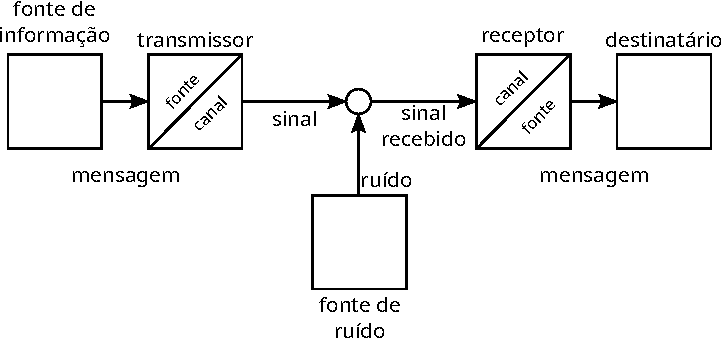
\includegraphics[width=\linewidth]{figures/shannon-communication-system.pdf}
  \caption{Diagrama genérico de um sistema de comunicações.}
  \label{fig:shannon-communication-system}
\end{figure}

O diagrama ilustrado na \Cref{fig:shannon-communication-system} apresenta a
sistematização proposta por \textcite{shannon1948}, incluindo conceitos e aspectos
da comunicação já utilizados à época, mas trazendo uma abordagem sistemática
para o conceito de comunicação. Além disso, ele divide a tarefa do codificador
e decodificador em duas partes distintas: a codificação/decodificação de fonte
e a codificação/decodificação de canal. Essa separação permite abordar cada uma
dessas partes do sistema de comunicação de forma independente, possibilitando,
assim, projetar e otimizar cada uma delas separadamente.

Para lidar matermaticamente com a comunicação, um processo que envolve
incerteza e variabilidade, e trazer então uma perspectiva probabilística na
abordagem do problema, inicialmente, é essencial entender o conceito de
variável aleatória (v.a.). Uma variável aleatória é uma variável que pode
assumir diferentes valores dependendo de fatores aleatórios, ou seja, opera-se
um mecanismo não determinístico que torna impossível prever seu valor. Ela
representa a incerteza inerente a eventos ou processos aleatórios e pode ser
utilizada para modelar diversos experimentos, como o lançamento de um dado, a
previsão do tempo ou a sequência de caracteres em um texto. Na notação aqui
adotada, as variáveis aleatórias serão representadas por letras maiúsculas,
como, por exemplo, $X$. Uma variável aleatória discreta é aquela que pode
assumir valores em um conjunto enumerável. As realizações de uma v.a. se dão de
acordo com uma distribuição subjacente $p$, e assim dizemos que $X \sim p$.
Para representar o conjunto de valores que a variável aleatória pode assumir,
utilizaremos a letra em forma caligráfica $\mathcal{X}$, enquanto um valor
específico que a variável pode assume será denotado por uma letra minúscula,
como $x$. Assim, podemos descrever que a variável aleatória $X$ assume o valor
$x$ através do evento $\{X=x\}$. 

Dada uma v.a. $X$, em um alfabeto $\mathcal{X}$ de cardinalidade $N = \vert\mathcal{X}\vert$,
onde $\mathcal{X} = \{a_1,\ldots,a_N\}$ e $a_i$, $i=1,\ldots,N$, representa
cada um dos possíveis valores que a v.a. pode assumir com probabilidade $p_i$, ou seja,
$p_i = \Pr(X=a_i)$. A distribuição subjacente que rege a v.a. $X$ é
$p = \mathcal{P}_X = \{p_1, \ldots, p_N\}$, tal que $p_i \geq 0$ e $\sum_{i=1}^N p_i = 1$ ou,
de forma equivalente, $\sum_{x \in \mathcal{X}} \Pr(X=x) = 1$.


\textcite{hartley1928} introduziu a ideia de que a quantidade de informação pode
ser medida em termos de possibilidades. Hartley propôs que a informação é
diretamente proporcional ao logaritmo do número de estados possíveis de um
sistema, estabelecendo assim uma base para a quantificação da informação. A
medida de informação associada a uma variável aleatória $X$, com alfabeto de
tamanho $N$, é expressa por
%
\begin{equation}\label{eq-hartley}
I(X) = \log_b L ,
\end{equation}
%
onde $b$ é a base utilizada para medir tal informação. Para $b=2$, a informação
será medida em `bits' (nome sugerido por J.W. Tukey).

O conceito proposto por Hartley sobre a quantificação da informação é
diretamente consonante com a interpretação da capacidade representacional de
uma unidade de memória. Em termos práticos, uma unidade de memória com $n$ bits
é capaz de representar $2^n$ sequências binárias distintas, o que implica que
essa unidade possui $n$ bits de informação. Quando consideramos duas unidades
de memória, cada uma com $n$ bits, a capacidade total se torna $2n$ bits,
permitindo a representação de $2^{2n}$ sequências binárias distintas. Essa
relação demonstra que, conforme a quantidade de bits de memória aumenta, a
capacidade de representação de informações também cresce exponencialmente,
alinhando-se perfeitamente com a proposta de Hartley de que a informação é
medida em função do número de estados possíveis.

Um conceito fundamental que emerge na discussão sobre a teoria da informação é
a redundância, ou ainda, a previsibilidade. A redundância refere-se à parte da
informação que é repetitiva ou desnecessária para a compreensão, podendo ser
eliminada sem perda de significado. Enquanto, sob uma primeira vista, pode ser
vista como um desperdício de recursos, a redundância também desempenha um papel
crucial na detecção e correção de erros, permitindo que a informação seja
transmitida de forma mais confiável em ambientes ruidosos. Exemplo disso é a
redundância presente na comunicação escrita. Veja como o trecho a seguir pode
ser facilmente compreendido, mesmo com lacunas: ``Nda se mudria, o regim, si
era posívl, ms tmbém s muda d roupa sm trcar d pele.''\footnote{Trecho origial:
  ``Nada se mudaria; o regime, sim, era possível, mas também se muda de roupa
  sem trocar de pele. Comércio é preciso. Os bancos são indispensáveis. No
  sábado, ou quando muito na segunda-feira, tudo voltaria ao que era na
  véspera, menos a constituição.'' (cap. LXIV de Esaú e Jacó, Machado de
Assis).} A capacidade de compreender o trecho, apesar das palavras truncadas e
da ausência de letras, demonstra que a linguagem é intrinsecamente projetada
para lidar com a incerteza e a imperfeição no processo de transmissão. Se não
houvesse redundância, qualquer perda de informação tornaria a decodificação da
mensagem inviável, resultando em confusão e mal-entendidos.

Shannon, por outro lado, incorporou o conceito de redundância em sua análise da
informação. Ao considerar eventos com probabilidades distintas, é importante
notar que a incerteza associada a esses eventos não pode ser a mesma. Assim, a
incerteza não depende apenas do tamanho do alfabeto, mas também das
probabilidades associadas a cada evento. Para um evento $E_k$ com probabilidade
$p_k$, a quantidade de informação (medida em bits) associada a esse evento é
expressa pela fórmula
%
\begin{equation}\label{eq-info-prop}
I(E_k) = − \log_2 (p_k) . 
\end{equation}
%
Essa relação indica que eventos menos prováveis, ou seja, aqueles com
probabilidades mais baixas, geram uma maior quantidade de informação, pois sua
ocorrência é mais inesperada. Em contrapartida, eventos com alta probabilidade
resultam em uma quantidade menor de informação, refletindo a redundância
presente na comunicação. Essa compreensão da relação entre probabilidade e
informação é essencial para o desenvolvimento do conceito de entropia, que
serve como uma medida da incerteza, aleatoriedade e quantidade de informação
associada a uma variável aleatória.

\section{Entropia}\label{sec:entropy}

\textcite{shannon1948} propôs a entropia com forma de quantificar a incerteza
associada a uma v.a., fornecendo assim uma medida da aleatoriedade.
A entropia nos permite entender como a distribuição de probabilidades de uma
variável aleatória influencia na informação associada a ela. A
entropia de uma v.a. é então expressa como o valor esperado da informação própria
associada aos eventos no alfabeto desta v.a., ou seja, $E_p[I(E_k)]$ e será
expressa por $H(X)$.
\begin{definition}[Entropia]
\begin{subequations}\label{eq:entropy-def}
\begin{align}
  H(X) \: &\triangleq \: \E_p \left[ -\log(p_k) \right] \\
       & = - \sum_{k=1}^{\vert \mathcal{X} \vert} p_k \log p_k \\
       & = - \sum_{x \in \mathcal{X}} p(x) \log p(x) ,
\end{align}
\end{subequations}
\end{definition}
Passamos a adotar a convenção $\log = \log_2$, uma vez que estaremos
sempre medindo a informação em bits. Quando necessário utilizar uma base
diferente, expressaremos explicitamente.

Para encontrar a formulação dada na \Cref{eq:entropy-def},
\textcite{shannon1948} propôs uma função de entropia $H$, que depende da
distribuição de massa $p$. Dado um alfabeto de tamanho $N = \mathcal{X}$, e
distribuição $p = \{p_1,\ldots,p_N\}$, Shannon estabeleceu três propriedades
fundamentais que a função de entropia deveria satisfazer. A primeira
propriedade exige que $H$ seja contínua em relação às probabilidades $p_i$, o
que significa que pequenas mudanças nas probabilidades não devem causar grandes
saltos na medida de informação. A segunda propriedade afirma que, se todos os
$p_i$ são iguais, a entropia deve aumentar monotonicamente com o tamanho do
alfabeto $N$. Isso reflete a intuição de que mais opções disponíveis para
escolha devem resultar em maior incerteza e, portanto, maior entropia. Por fim,
a terceira propriedade, conhecida como a propriedade da aditividade, estabelece
que se uma escolha pode ser decomposta em uma sequência de escolhas
independentes, a entropia total deve ser a soma ponderada das entropias
individuais de cada escolha. Essa propriedade é crucial para a análise de
sistemas complexos, onde a informação pode ser tratada em partes menores e
combinadas para obter uma visão global.

A formulação matemática da entropia de Shannon, dada na \Cref{eq:entropy-def},
emerge naturalmente ao considerar essas propriedades, sendo a função
logarítmica utilizada devido à sua capacidade de transformar multiplicações em
somas, o que é essencial para garantir a aditividade da medida de informação.

\begin{interlude}
  \label{beginof:interlude:appendix2}
  Este interlúdio fornece uma pausa para apresentar a demonstração contida no
  Anexo 2 do artigo de \textcite{shannon1948}.  O leitor, se desejar, pode ir
  direto à página \pageref{endof:interlude:appendix2}, onde finaliza-se este
  entreato.

  Define-se a $A(N)$ como o caso específico de $H$ para uma distribuição
  uniforme com alfabeto de tamanho $N$:
  \begin{equation}
  A(N) = H\left( \frac{1}{N}, \frac{1}{N}, \ldots, \frac{1}{N} \right) .
  \end{equation}

  Deseja-se que uma escolha dentre $s^M$ opções igualmente prováveis possa ser
  decomposta como uma sequência de $M$ escolhas que se subdividem em $s$
  possibilidades igualmente prováveis.

  Teremos então que
  \begin{equation}
  A(s^M) = M A(s) .
  \end{equation}
  Da mesma forma, para $t$ e $N$, teremos $A(t^N) = N A(t)$.
  Podemos tomar $N$ arbitrariamente grande e encontrar $M$ que satisfaça
  \begin{equation}
  s^M \leq t^N \leq s^{(M+1)} .
  \end{equation}
  Tomando o logaritmo\footnote{Logaritmo é uma função monótona crescente.} da
  expressão acima e dividindo por $N \log s$ todos os termos\footnote{
      $N \log s$ é positivo para $N \geq 0$ e $s \geq 1$.
  }, teremos
  \begin{equation}
  \frac{M}{N} \leq \frac{\log t}{\log s} \leq \frac{M}{N} + \frac{1}{N} ,
  \end{equation}
  o que é equivalente a
  \begin{equation}
  \left\vert \frac{M}{N} - \frac{\log t}{\log s} \right\vert < \epsilon ,
  \end{equation}
  onde $\epsilon$ é arbitrariamente pequeno, já que $N$ é arbitrariamente
  grande.

  Usando agora a propriedade desejada de monotonicidade de $A(N)$, teremos
  \begin{subequations}
  \begin{alignat}{3}
  A(s^M) &\leq A(t^N) &\leq A(s^{(M+1)}) \\
  M \, A(s) &\leq N \, A(t) &\leq (M+1)A(s)
  \end{alignat}
  \end{subequations}

  Dividindo a expressão acima por $NA(s)$, teremos
  \begin{equation}
  \frac{M}{N} \leq \frac{A(t)}{A(s)} \leq \frac{M}{N} + \frac{1}{N} ,
  \end{equation}
  ou, de forma equivalente,
  \begin{equation}
  \left\vert \frac{M}{N} - \frac{A(t)}{A(s)} \right\vert < \epsilon ,
  \end{equation}
  e assim, como as duas frações ($\sfrac{\log t}{\log s}$ e
  $\sfrac{A(t)}{A(s)}$) estão $\epsilon$ próximas de $\sfrac{M}{N}$,
  podemos concluir que
  \begin{equation}
  \left\vert \frac{A(t)}{A(s)} - \frac{\log t}{\log s} \right\vert < 2\epsilon .
  \end{equation}
  Como $\epsilon$ é arbitrariamente pequeno, no limite teremos
  \begin{subequations}
  \begin{align}
  \frac{A(t)}{A(s)} &= \frac{\log t}{\log s} \\
  A(t) &= \frac{A(s)}{\log s} \log t = K \log t ,
  \end{align}
  \end{subequations}
  onde $K$ deve ser positivo, de forma que $A(N)$ seja monótona crescente.

  Suponha uma escolha com $N$ possibilidades em que as probabilidades são
  comensuráveis, $p_i = \sfrac{N_i}{\sum N_i}$, onde $N_i$ são inteiros. De
  forma equivalente, uma escolha entre $\sum N_i$ opções pode ser expressa como
  uma escolha dentre $N$ opções com probabilidades $p_1, \ldots, p_N$, e para
  uma $i$-ésima dada escolha, realizar uma nova escolha dentre $N_i$ opções
  igualmente prováveis. Teremos então:
  \begin{subequations}
  \begin{align}
  \overbrace{ K \log \left( \sum N_i \right) }^{A\left( \sum N_i \right)} &= H(p_1, \ldots, p_N) + \overbrace{ K \log N_i }^{A(N_i)} \\
  K \underbrace{\left( \sum p_i \right)}_{=1} \log \left( \sum N_i \right) &= H(p_1, \ldots, p_N) + K \underbrace{\left( \sum p_i \right)}_{=1} \log N_i .
  \end{align}
  \end{subequations}
  E assim,
  \begin{subequations}
  \begin{align}
  H(p_1, \ldots, p_N) &= K\left[ \left( \sum p_i \right) \log \left( \sum N_i \right) - \left( \sum p_i \right) \log N_i \right] \\
        &= -K \sum p_i \log \frac{N_i}{\sum N_i} = -K \sum p_i \log p_i . \qed
  \end{align}
  \end{subequations}
  \label{endof:interlude:appendix2}
\end{interlude}

Tomemos primeiramente um exemplo simples de uma v.a. binária $X \in \mathcal{X} = \{0,1\}$.
Para simplificar, iremos denotar arbitrariamente por $\theta = Pr(X=1)$ e $1-\theta = Pr(X=0)$.
Usando agora a definição dada na \Cref{eq:entropy-def}, teremos
\begin{equation}\label{eq:entropia-binaria}
H(X) = -\theta \log \theta - (1-\theta) \log (1-\theta)
\end{equation}
e, para simplificar, iremos denotar esta grandeza por $H(\theta)$.
Sempre que utilizarmos esta notação, como por exemplo em $H(\sfrac{1}{4})$, $H(\sfrac{1}{3})$ ou $H(\pi)$,
estaremos nos referindo à entropia binária definida na \Cref{eq:entropia-binaria}.

\begin{marginfigure}%
  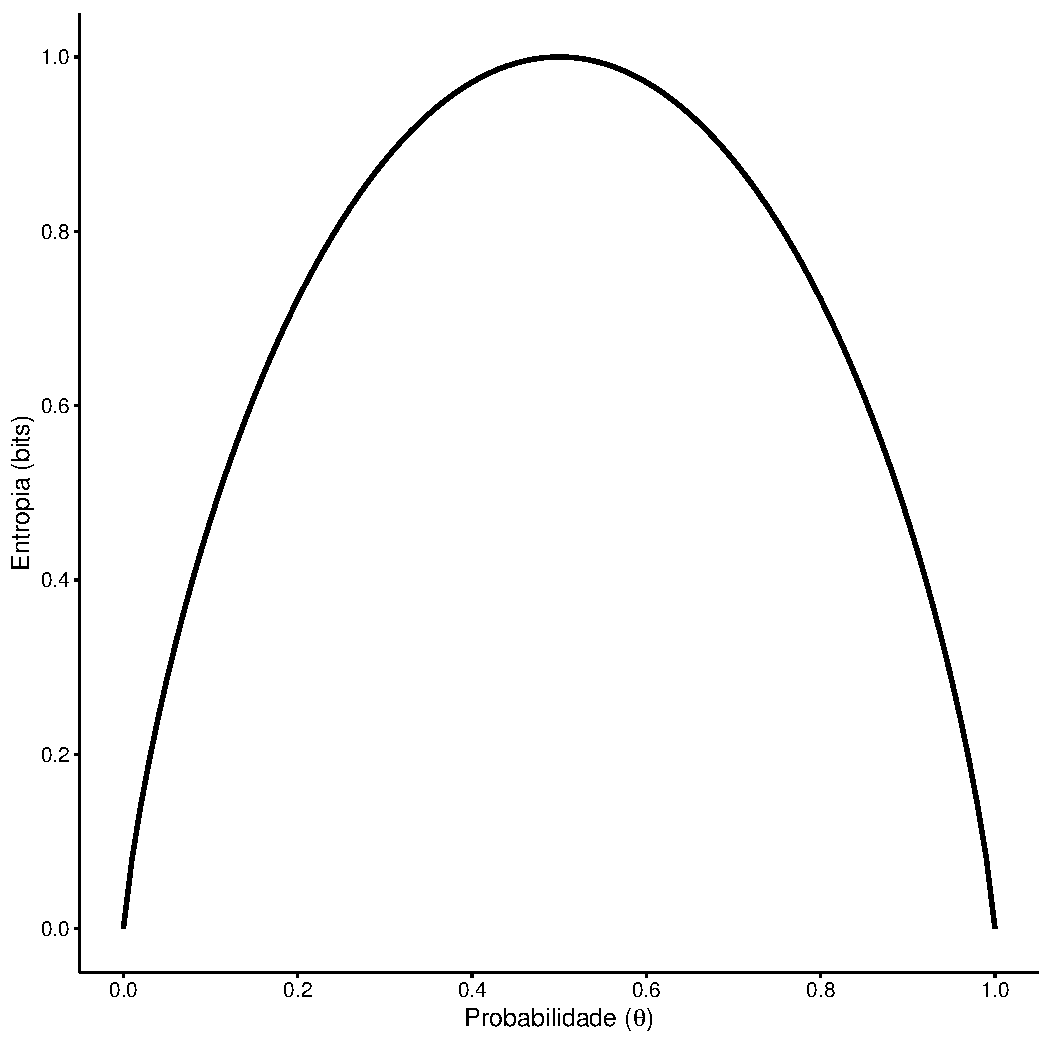
\includegraphics[width=\linewidth]{plots/binary_entropy.pdf}
  \caption{Entropia binária}
  \label{fig:entropiabinaria}
\end{marginfigure}

A \Cref{fig:entropiabinaria} apresenta o gráfico da entropia binária dada pela
\Cref{eq:entropia-binaria}. Note como $H=0$ quando $\theta = 1$ ou $\theta =
0$, ou seja, nos casos em que um dos eventos ocorre com probabilidade 1.
Observe ainda como o máximo é alcançado em $\theta = \sfrac{1}{2}$, quando
ambos eventos são equiprováveis (máxima incerteza). A função observada é
côncava, o que, mais à frente, mostraremos ser válido para toda função de
entropia. A concavidade garante ainda que ao misturarmos (ponderarmos)
distribuições diferentes não é possível obter uma entropia menor que a
ponderação das entropias das partes.

Vamos considerar agora o exemplo de uma v.a. com distribuição uniforme $X \sim u$.
Usando a definição na \Cref{eq:entropy-def}, teremos que a entropia de $X$ será dada por
\begin{subequations}\label{eq:entropy-uniform}
\begin{align}
    H(X) \: &= - \sum_{k=1}^{\vert \mathcal{X} \vert} \frac{1}{\vert \mathcal{X} \vert} \log \frac{1}{\vert \mathcal{X} \vert} \\
            &= - \log \sfrac{1}{\vert \mathcal{X} \vert} = \log \vert \mathcal{X} \vert .
\end{align}
\end{subequations}
Como esperávamos, a entropia de uma distribuição uniforme é monotonicamente
crescente com o tamanho do alfabeto. Intuitivamente, como já mencionado,
a entropia é máxima para uma distribuição uniforme, uma vez que é a situação
de maior incerteza para um dado alfabeto.

Ao analisarmos a \Cref{eq:entropy-def}, podemos nos questionar o que ocorre
quando algum símbolo tem probabilidade zero, uma vez que aparecerá um termo
$0 \log 0$ no somatório. Neste caso, iremos usar o valor limite $\lim_{x \rightarrow 0} x \log x = 0$.
Para demonstrar (a menos de uma constate pela mudança de base do logaritmo), 
usaremos para tanto a regra de L'Hospital:
\begin{subequations}\label{eq:0log0}
\begin{align}
    \lim_{x \rightarrow 0} x \ln x \: &= \lim_{x \rightarrow 0} \frac{\ln x}{\sfrac{1}{x}} \\
				    &= \lim_{x \rightarrow 0} \frac{\sfrac{1}{x}}{-\sfrac{1}{x^2}} \\
				    &= \lim_{x \rightarrow 0} -x = 0.
\end{align}
\end{subequations}

No próximo exemplo, vamos buscar aproximar a entropia de textos escritos.
Sabemos que a distribuição das palavras em textos segue uma lei de potência
conhecida como Lei de Zipf
\cite{zipf1935,zipf1949,FerreriCancho2001,araujo2013}.  A Lei de Zipf é uma
observação empírica que também é observada em diversos outros naturais.  Ao
analisar um corpus de texto, Zipf constatou que a frequência de uma palavra é
inversamente proporcional à sua posição em um ranking de frequência.  Essa
relação pode ser expressa matematicamente como 
\begin{equation}\label{eq:zipf}
    p_k(s, N) \: = C \, k^{-s},
\end{equation}
onde $p_k$ é a probabilidade de ocorrência da $k$-ésima palavra mais frequente,
$C$ é uma constante de normalização ($C^{-1} = \sum_{n=1}^N n^{-s}$), $k$ é o
\emph{rank}, $s$ a constante que caracteriza a distribuição e $N$ o tamanho do
léxico. A \Cref{fig:zipfshakespeare} apresenta o gráfico de Zipf
(frequência/probabilidade vs. \emph{rank}) para a obra completa de William
Shakespeare, dividida em 44 textos, conforme organizados no Projeto
Gutenberg\footnote{\url{https://www.gutenberg.org/}}.  Cada uma das série de pontos na
\Cref{fig:zipfshakespeare} representa um destes 44 textos.  Note como o
comportamento observado entre eles é bem similar.

% script to create the figure
% leoca@r2d2:~/ee/research/clscripts$ ./multiple_zipf_plot.sh --probability /ms/downloads/samples/gutenberg/shakespeare/shakespeare*
\begin{figure}%
    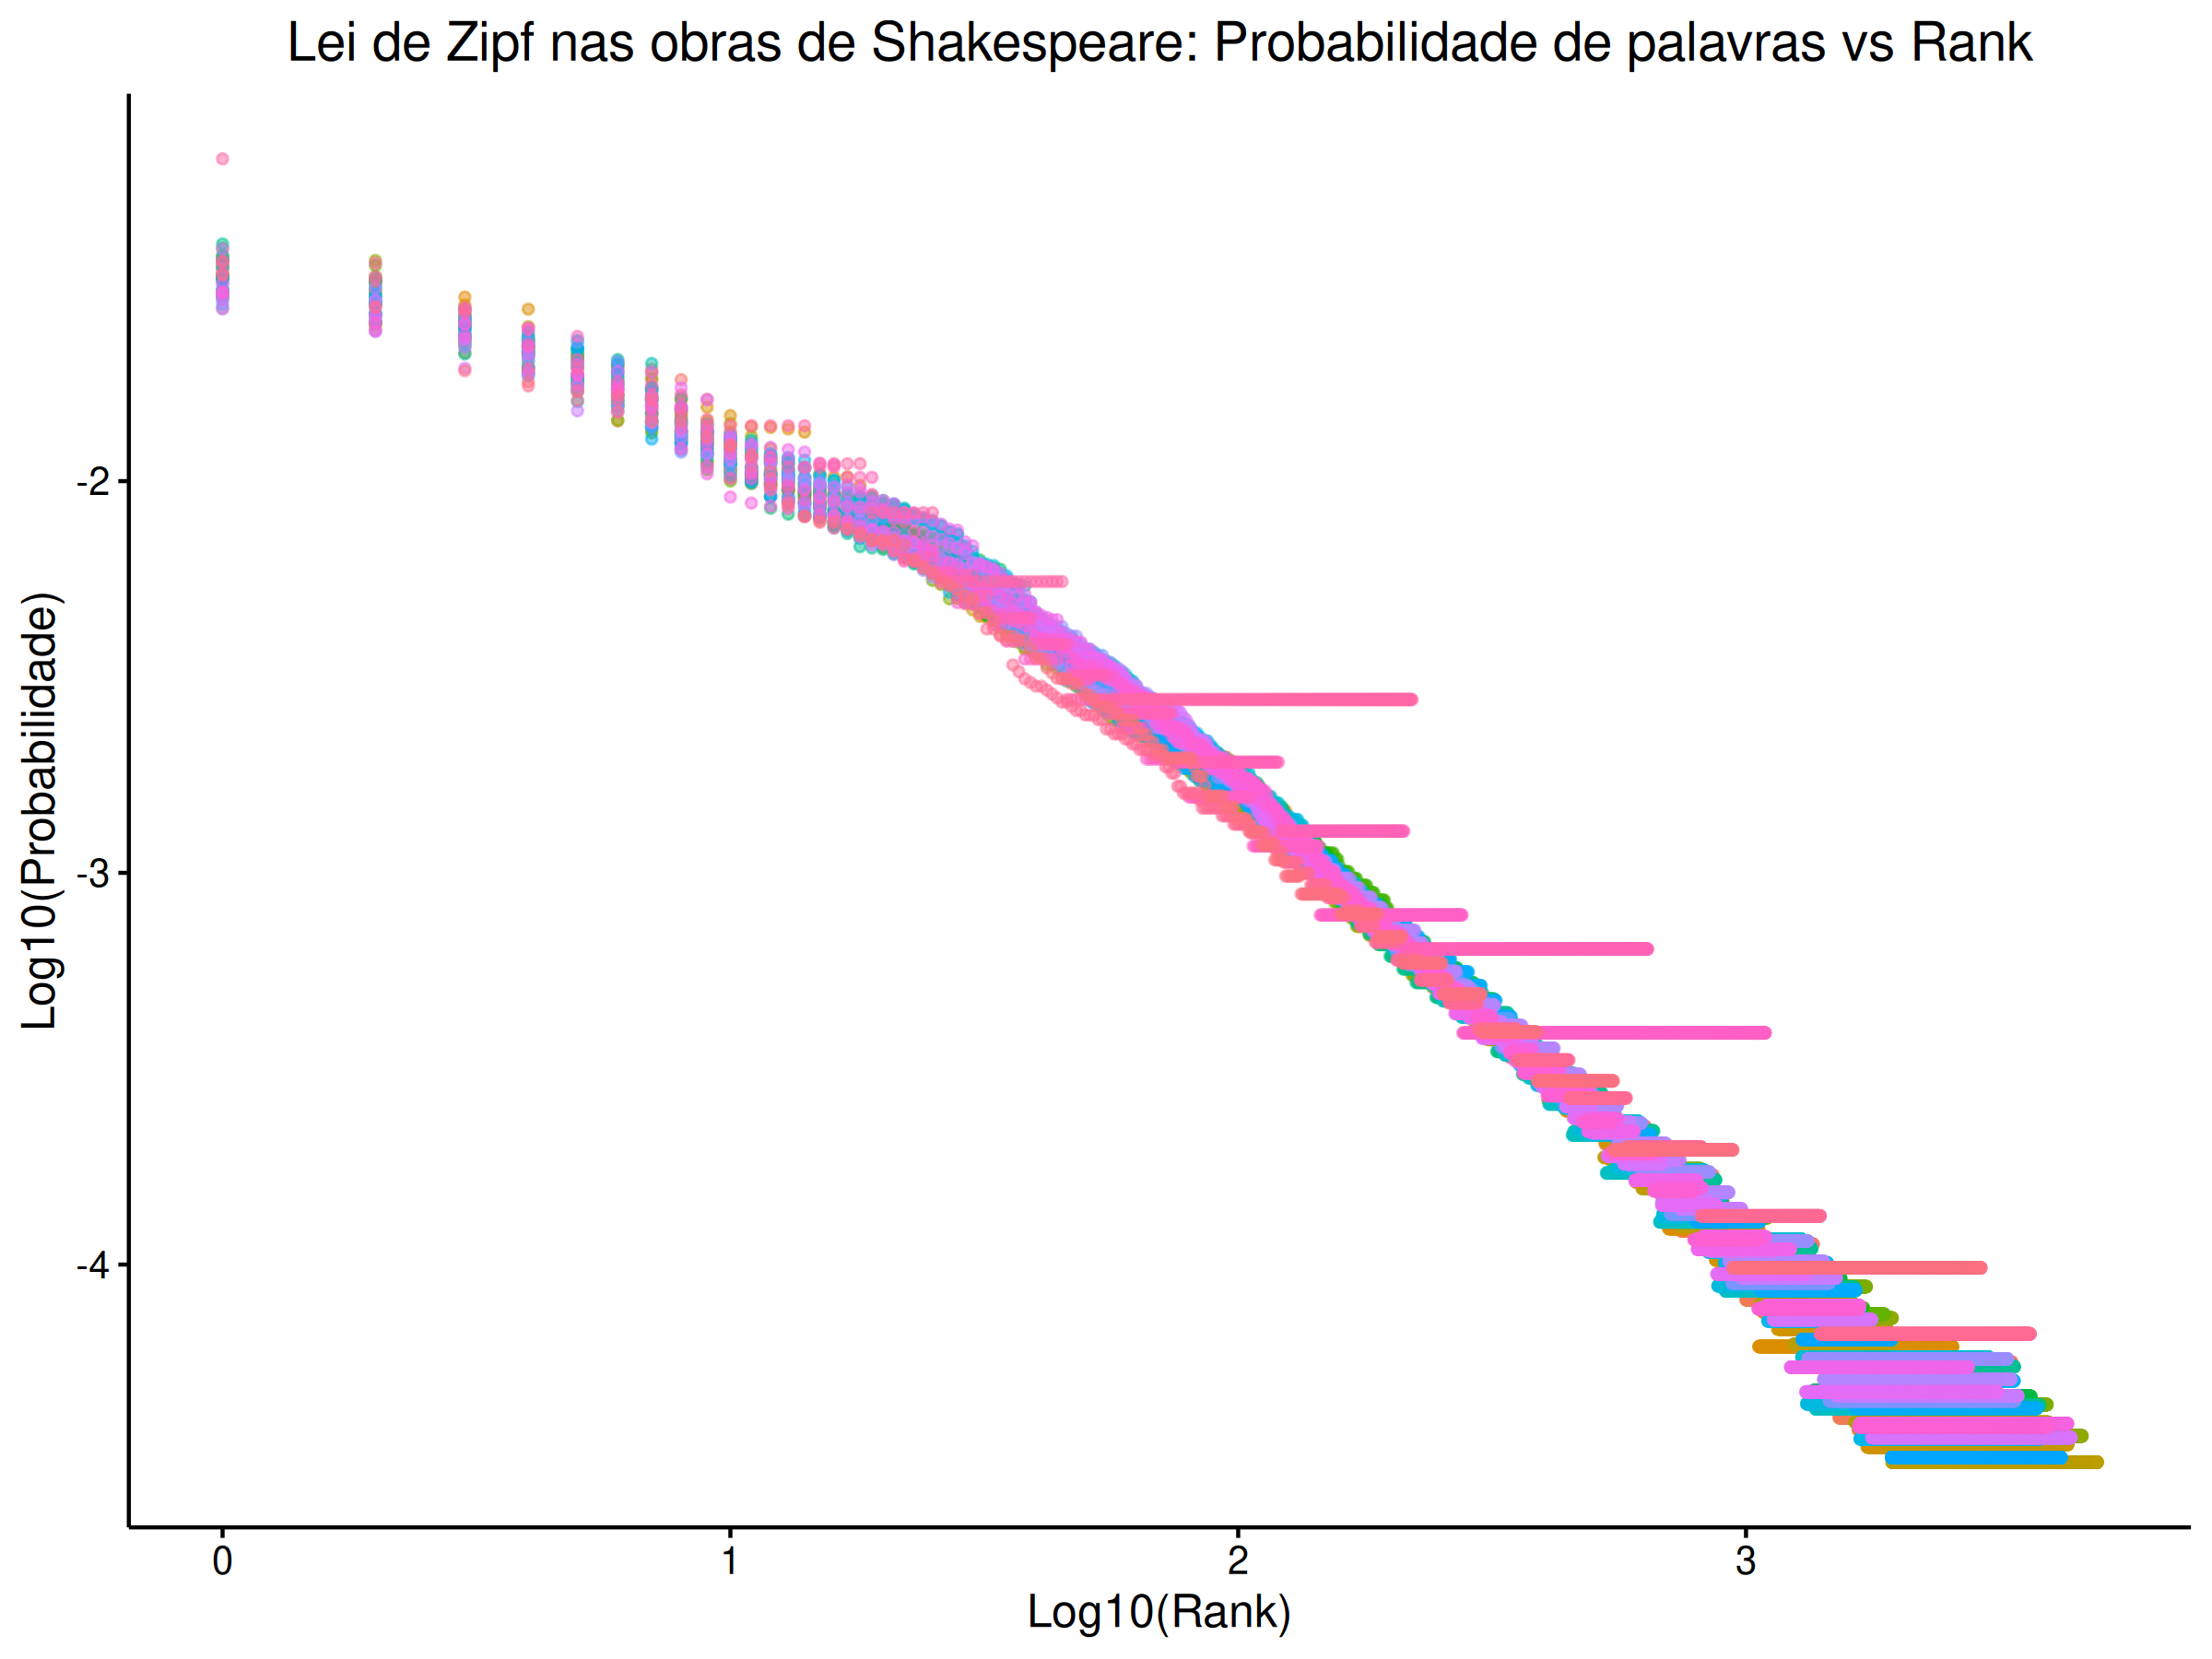
\includegraphics[width=\linewidth]{figures/zipf_plot.png}
    \caption{Gráfico de Zipf para 44 textos de William Shakespeare no Projeto Gutenberg.}
    \label{fig:zipfshakespeare}
\end{figure}


Usando a \Cref{eq:zipf} em conjunto com a \Cref{eq:entropy-def}, obtemos a
formulação da entropia para uma distribuição de Zipf:
\begin{equation}\label{eq:zipf-entropy}
H(X) \: = s \, C \sum_{k=1}^{N} \frac{\log k}{k^s} - \log C .
\end{equation}
Após estimar a entropia de cada um dos textos de Shakespeare, podemos observar
no histograma da \Cref{fig:zipfshakespeareentropy} como a concentração dos valores
encontrados está por acima de 9 bits. Como observaremos mais à frente, conhecer
o valor da entropia é importante para sabermos qual é o limite representacional
para uma fonte (qual é o limite da compressão). Além disso, linguistas utilizam
a entropia para analisar a complexidade de uma língua, redundância e eficiência
do sistema de escrita.

% script to create the figure
% leoca@r2d2:~/ee/research/clscripts$ for file in $(ls /ms/downloads/samples/gutenberg/shakespeare/*); do ./wordcounttfl.sh -c -i $file | ./entropy.py; done | ./histogram.R
\begin{marginfigure}%
    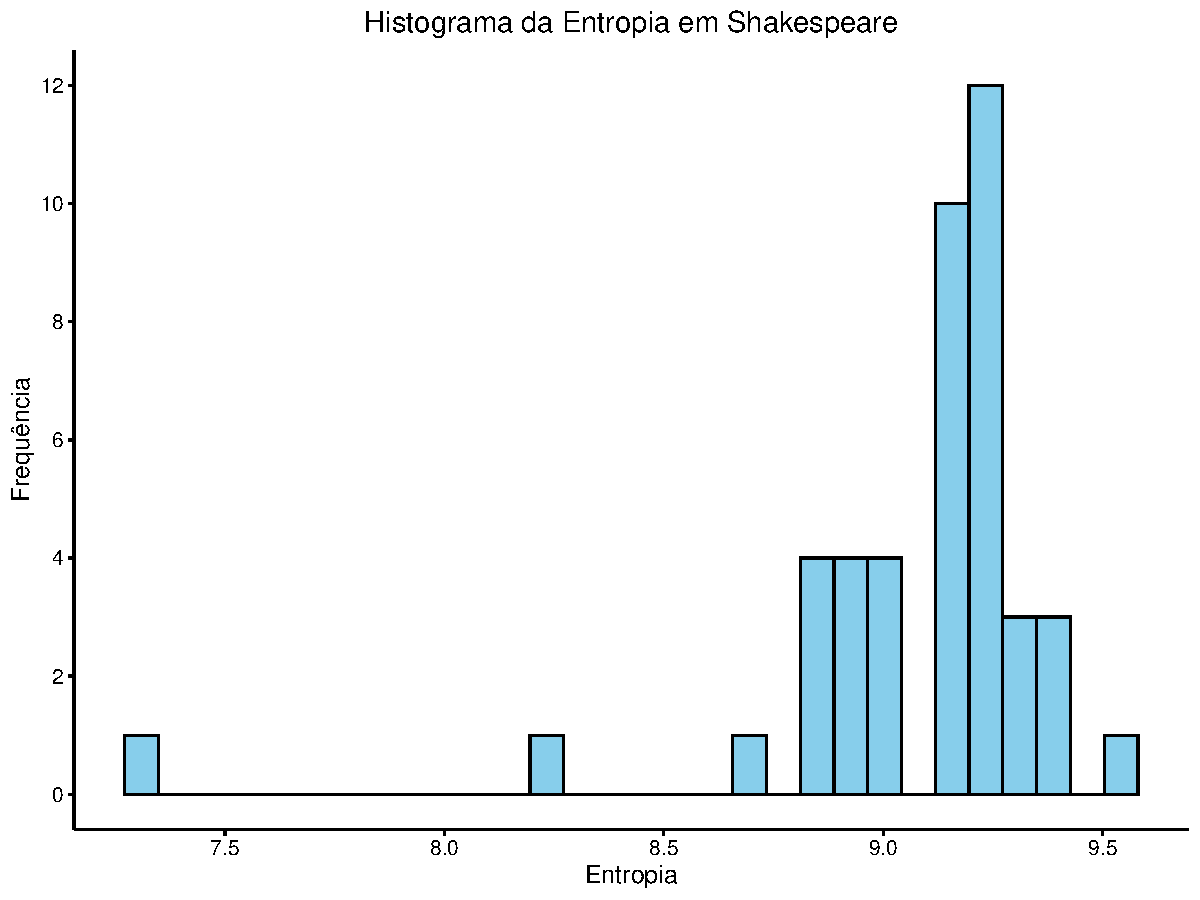
\includegraphics[width=\linewidth]{figures/zipf_entropy_shalespeare.pdf}
    \caption{Histograma da entropia nos 44 textos de William Shakespeare.}
  \label{fig:zipfshakespeareentropy}
\end{marginfigure}









\section{Propriedades da Entropia}\label{sec:entropyprop}

A entropia possui várias propriedades fundamentais que iremos descrever a
seguir. Essas propriedades não apenas ajudam a entender o comportamento da
entropia e medidas relacionadas, como também serão uteis em diversas
demonstrações. Nesta seção, exploraremos as principais propriedades da
entropia, incluindo a não negatividade, a concavidade, valor máximo, a
continuidade, e a mudança de base.

Como dito anteriormente, usualmente a unidade escolhida para medir a informação
é bit, e portanto utilizamos a base $2$. Entretanto, a entropia pode ser dada
também em outras bases: nats (base $e$), trits (base $3$), hartley (base $10$).
Para obtermos a entropia em outras bases, basta utiliza a regra de mudança de
base do logaritmo: $\log_{a} x = \sfrac{\log_{b} x}{\log_{b} a}$. Teremos
assim $H_b(X) = (\log_b a) H_a(X)$. A transformação para a base $e$ costuma ser
útil nas demonstrações para evitar o fardo de se carregar uma constante durante
todo o seu percurso.

Uma propriedade muito importante é a não negatividade, ou seja, $H(X) \geq 0$.
A incerteza nunca\footnote{Importante ressaltar que estamos aqui tratando de
    variáveis discretas. No contexto contínuo a entropia pode ser negativa e
    terá outra interpretação.} 
será negativa, o que faz sentido intuitivamente.  Além disso, a não
negatividade é uma propriedade importante para encontrarmos outras relações.
Para verificá-la, basta notar que a entropia é a soma de termos da forma $-p
\log p$, como $0 \leq p \leq 1$, teremos que cada termo da soma é maior ou
igual a zero. Por conseguinte, a entropia seria não negativa.

Para verificar que a entropia é uma função contínua em $p$, devemos primeiramente
definir $l(x)$ como a extensão contínua de $x \log x$, da seguinte forma:
\begin{equation}
l(x) \: = \begin{cases}
      x \log x & \quad \text{se } x > 0 , \\
      0        & \quad \text{se } x = 0 ,
      \end{cases}
\end{equation}
e assim, $H(X) = H(p)$ é definido como
\begin{equation}
H(p) = - \sum_{x \in \mathcal{X}} l(p_x) .
\end{equation}
Sendo a entropia definida como um somatória finito de funções contínuas,
fica evidente que ela também será uma função contínua.

Antes de abordarmos uma próxima propriedade fundamental da entropia, vamos
estabelecer uma desigualdade simples e importante em diversas demonstrações
futuras. Ela é apresentada graficamente na \Cref{fig:lnzzm1} e demonstrada
formalmente no \Cref{lm:desfundamental}.
% script to create the figure
% lnzzm1.R
\begin{marginfigure}%
    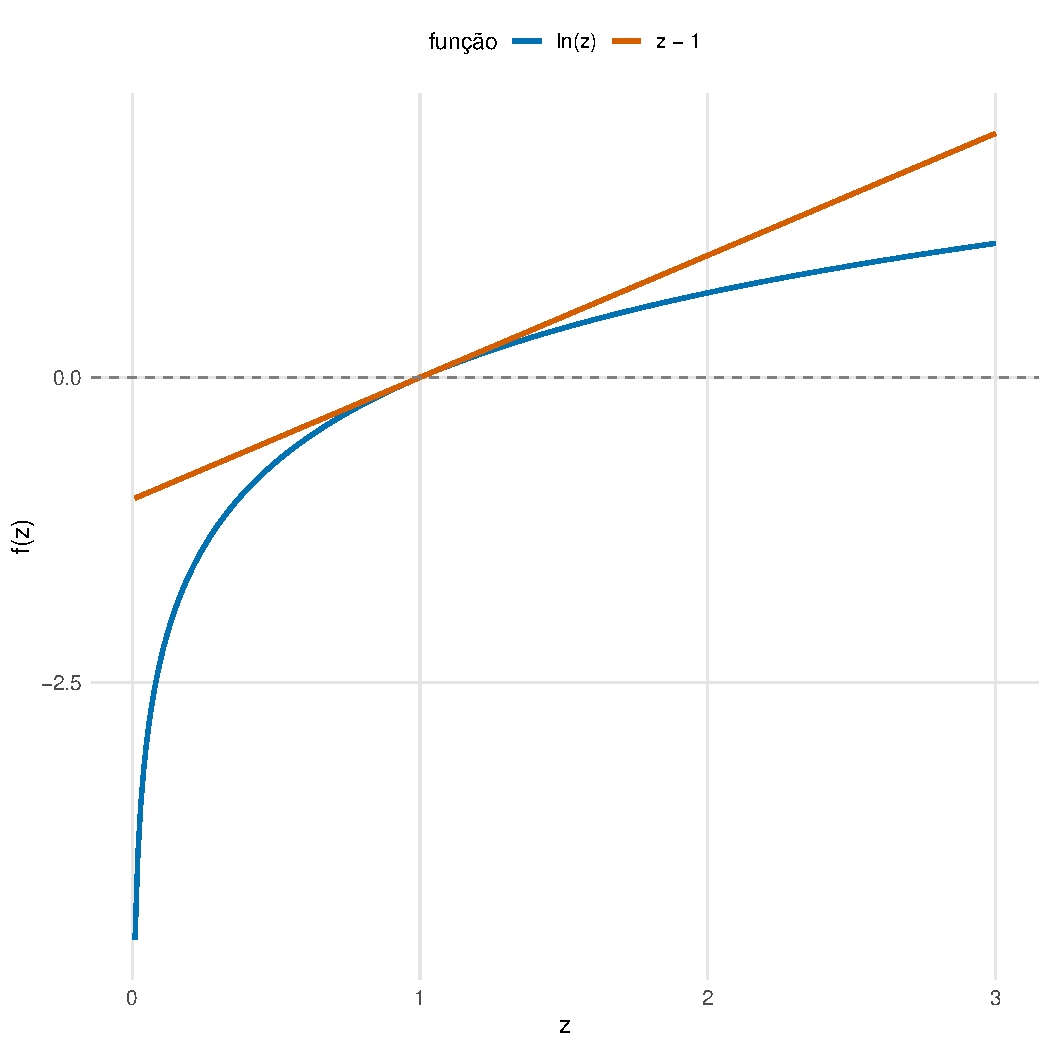
\includegraphics[width=\linewidth]{plots/lnzzm1.pdf}
    \caption{Demonstração gráfica da desigualdade $\ln z \leq z - 1$ (embora
    não seja uma demonstração formalmente válida, serve como intuição).}
    \label{fig:lnzzm1}
\end{marginfigure}
\begin{lemma}[Desigualdade Fundamental]\label{lm:desfundamental}
Para qualquer $z > 0$,
\begin{equation}\label{eq:fund-ineq}
    \ln z \leq z - 1,
\end{equation}
com igualdade se e somente se $z = 1$.
\end{lemma}
\begin{proof}
Sabemos que para $z = 1$ é verdadeiro, pois $0 = \ln 1 \leq 1 - 1 = 0$.
Vamos demonstrar que $\ln z \leq z-1$, para $z \geq 1$ por contradição.
Suponha que existe $b > 1$ tal que $\ln z > z - 1$, para $z=b$.
Vamos definir $f(z) = \ln z - z + 1$, logo $f(1) = 0$ (conforme visto acima)
e $f(b) > 0$ (por hipótese).
Pelo teorema do valor médio $\exists c$, $1 < c < b$, tal que
\begin{equation}
f'(c) = \frac{f(b) - f(1)}{b - 1} = \frac{\overbrace{f(b)}^{>0}}{\underbrace{b-1}_{>0}} > 0 .
\end{equation}
Mas, $f'(z) = 1/z -1$, e assim $f'(z) < 0$ para $z>1$. Logo há uma contradição
e nossa hipótese é falsa. Teremos assim $\ln z \leq z-1$, para $z \geq 1$.

Para $z \in (0,1)$, basta seguir os mesmos passos, escolhendo um ponto
$z=b$, tal que $0 < b < 1$. Vamos encontrar um ponto $c$ tal que $0 < b < c < 1$.
E usar o teorema do valor médio para mostrar uma contradição na hipótese.
\end{proof}

Outra propriedade importante que mencionamos é o limite máximo da entropia,
a entropia da distribuição uniforme. Note que, mostrar que $H(X) \leq \log N$
é equivalente a mostrar que $H(X) - \log N \leq 0$. Para tanto, vejamos:
\begin{subequations}\label{eq:demlimentropy}
\begin{align}
H(X) - \log N \: &= - \sum_x p(x) \log p(x)  - \log N \overbrace{\sum_x p(x)}^{=1} \\
    &= - \sum_x p(x) \log p(x) - \sum_x p(x) \log N \\
    &= - \sum_x p(x) \log p(x) \, N \\
    &= \log_2 e \sum_x p(x) \ln \frac{1}{p(x) N} \\
    &\leq \log_2 e \sum_x p(x) \left[ \frac{1}{p(x) N} -1 \right] \\
    &= \log_2 e \left[ \underbrace{\sum_{x \in \mathcal{X}} \frac{1}{N}}_{= N \frac{1}{N} = 1} - \underbrace{\sum_x p(x)}_{=1} \right] = 0. \qed
\end{align}
\end{subequations}
Na demonstração anterior, utilizamos a \Cref{eq:fund-ineq}, com $z = \sfrac{1}{p(x) \, N}$.
A igualdade $\ln z = z-1$ se dará no ponto $z = 1$, isto é, quando $\sfrac{1}{p(x) \, N} = 1$, ou seja,
quando $p(x) = \sfrac{1}{N}$, e teremos assim uma distribuição uniforme.

A concavidade da entropia é uma propriedade importante. Garante que a entropia
terá um único máximo global. A maximização da entropia é um princípio
fundamental em várias áreas como estatística, para a inferência de
distribuições de probabilidade, e aprendizado de máquina, para garantir que os
algoritmos de otimização convirjam e para garantir a estabilidade dos modelos.
Esta propriedade será demonstrada mais à frente.



\section{Entropia Conjunta e Entropia Condicional}\label{sec:entropiaconjunta}

Quando lidamos com incerteza em situações que envolvem múltiplas variáveis aleatórias,
entropia conjunta e a entropia condicional são conceitos que surgem da extensão das definições
vistas anteriormente. Um par de varáveis aleatórias $(X,Y)$ pode ser visto como
uma variável aleatória vetorial.

A entropia conjunta de duas variáveis aleatórias $X$ e $Y$, denotada como $H(X,Y)$, 
mede a incerteza total associada ao par de variáveis. É definida como:
\begin{definition}[Entropia Conjunta]
\begin{subequations}\label{eq:jointentropy}
\begin{align}    
H(X,Y) \: &\triangleq - \sum_{x \in \mathcal{X}} \sum_{y \in \mathcal{Y}} p(x,y) \log p(x,y) \\
	  &= \E_{p(x,y)} \log \frac{1}{p(X,Y)} \\
	  &= \E \log \frac{1}{p(X,Y)},\label{eq:jointentropysimpl}
\end{align}
\end{subequations}
onde, em \ref{eq:jointentropysimpl}, para simplificar\footnote{Tais simplificações pode
aparecer ao longo do texto. Porém as adotaremos apenas em casos que não gerem ambiguidades.}, 
omitimos a distribuição em respeito
a qual o valor esperado é tomado.
\end{definition}

Generalizando para um vetor de variáveis aleatórias $X_{1:N} = (X_1, X_2, \ldots, X_N)$:
\begin{subequations}\label{eq:entropiavetor}
\begin{align}
H(X_{1:N}) \: &= H(X_1, X_2, \ldots, X_N) \\
     &= \sum_{x_1, x_2, \ldots , x_N} p(x_1, \ldots, x_N) \log \frac{1}{p(x_1, \ldots, x_N)} \\
     &= \E \log \frac{1}{p(X_1, \ldots, X_N)} .
\end{align}
\end{subequations}

Dada a definição, vamos analisar um exemplo prático para analisar a
interdependência entre caracteres consecutivos em uma língua natural. Para
calcular a entropia conjunta de dois caracteres em sequência, devemos
primeiramente calcular a probabilidade conjunta. A
\Cref{fig:jointprobabilityshakespeare} apresenta o resultado encontrado para a
obra completa de Shakespeare. Note como os maiores valores correspondem às
sequências `th', `he', `er', `an', dentre outras (devido às palavras de alta
frequência de ocorrência na língua, como ``the'', ``in'', ``her'', ``there'',
etc.

Ao calcular a entropia conjunta encontramos $H(X,Y) = 7.8482$~bits, o que é
menor do que o dobro da entropia de um único caractere, $2 \times H(X) = 8.3798$~bits. 
O fato da entropia conjunta de dois caracteres consecutivos ser
menor do que o dobro da entropia de um único caractere indica que os caracteres
não são independentes: a ocorrência de um caractere influencia a probabilidade
do próximo, reduzindo a incerteza total. Em uma língua natural, essa
interdependência é esperada devido a padrões linguísticos.

% script to create the figure
% ~$ cat /ms/downloads/samples/gutenberg/shakespeare/* > /tmp/text.txt
% R: joint_probability.R
\begin{figure}%
    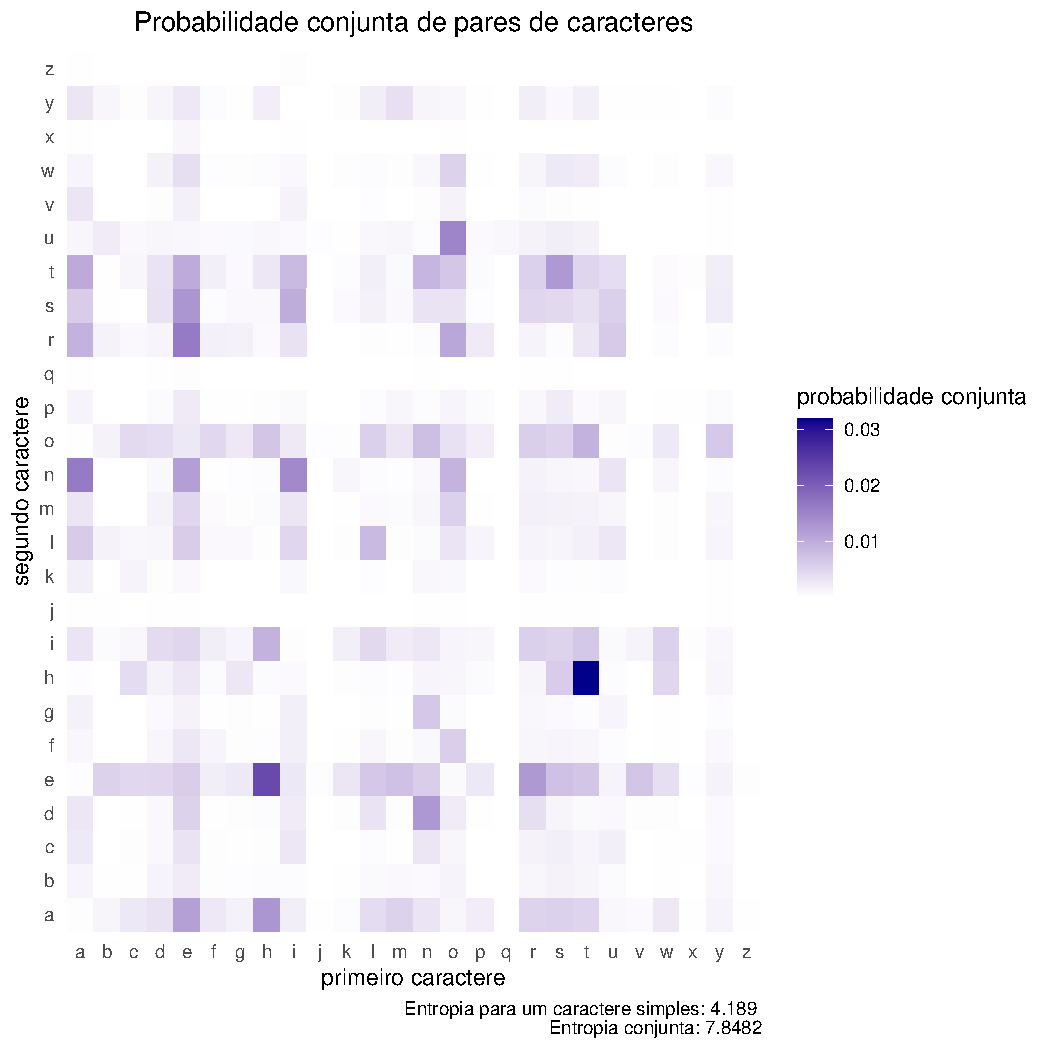
\includegraphics[width=\linewidth]{plots/joint_probability.pdf}
    \caption{Probabilidade conjunta do primeiro e segundo caractere analisando os 44 textos de William Shakespeare no Projeto Gutenberg. As entropias simples e conjunta são apresentadas, evidenciando que a entropia conjunta é maior, porém, analisando a entropia por caractere, a entropia conjunta abarca dependências entre caracteres consecutivos, reduzindo o efeito de incerteza por caractere.}
    \label{fig:jointprobabilityshakespeare}
\end{figure}


Essa interdependência sugere que a incerteza associada ao segundo caractere
($Y$), dado o conhecimento do primeiro caractere ($X$), é menor do que a
incerteza do segundo ($Y$) quando considerado isoladamente. Em outras palavras,
o conhecimento de $X$ fornece informação que reduz a incerteza sobre $Y$, como
ocorre em pares comuns como `th', onde `t' aumenta a probabilidade de `h'. Essa
incerteza reduzida é formalmente chamada de entropia condicional, denotada por
$H(Y|X)$, e é definida como
\begin{definition}[Entropia Condicional]
\begin{subequations}\label{eq:entropiacondicional}
\begin{align}
 H(Y|X) \: &\triangleq \sum_x p(x) H(Y|X=x) \label{eq:entcondevents} \\
        &= - \sum_x p(x) \sum_y p(y|x) \log p(y|x) \\
	&= - \sum_{x,y} p(x,y) \log p(y|x) \label{eq:entcondsumPs}\\
	&= \E_{p(x,y)} \log \frac{1}{p(Y|X)}.
\end{align}
\end{subequations}
\end{definition}

A definição dada pela \Cref{eq:entcondevents} nos mostra como a entropia
condicional de $Y$, dado $X$, é o valor esperado da entropia de $Y$
condicionada aos eventos $x$.  Observamos anteriormente (e será demonstrado
posteriormente) que $H(Y|X) \leq H(Y)$, pois conhecer $X$ reduz a incerteza
sobre $Y$. Entretanto, devemos ressaltar que nada podemos dizer com relação a
$H(Y|X=x)$, podendo este ser menor, igual ou maior que $H(Y)$. Para um caso
específico, condicionar pode aumentar a incerteza, embora, na média, a entropia
condicional seja sempre menor ou igual a entropia sem ser condicionada. Um
exemplo interessante, adaptado de \textcite{cover2006}, é o contexto de um
julgamento: uma evidência única evidência pode aumentar a incerteza sobre um
determinado caso, o que pode levar a um julgamento enviesado; entretanto,
conhecer um conjunto de evidência nos leva esperar uma incerteza menor,
eliminando o viés no julgamento.

Note que, condicionando $H(Y|X)$ a $Z$, usando a \Cref{eq:entcondevents} podemos
escrever
\begin{equation}\label{eq:entcondeventsZ}
H(Y|X,Z) \: = \sum_z p(z) H(Y|X,Z=z),
\end{equation}
onde 
\begin{equation}\label{eq:entcondeventsZz}
H(Y|X,Z=z) \: = -\sum_{x,y} p(x,y|z) \log p(y|x,z) .
\end{equation}

Observando as definições de entropia conjunta e entropia condicional, surge, naturalmente,
a constatação de que a entropia de um par de variáveis aleatória é a entropia de uma
somada à entropia condicional da outra. Esta observação é formalizada pelo teorema
da regra da cadeia.

\begin{theorem}[Regra da Cadeia]\label{thm:regracadeia}
 \begin{equation}
  H(X,Y) = H(X) + H(Y|X) = H(Y) + H(X|Y)
 \end{equation}
\end{theorem}
\begin{proof}
 Como $p(x,y) = p(x) p(y|x)$ (teorema de Bayes), e como o logaritmo de um produto é a soma 
 dos logaritmos dos fatores, teremos
 \begin{equation}
 - \log p(x,y) = - \log p(x) - \log p(y|x)
 \end{equation}
 onde multiplicamos por $(-1)$ ambos os lados.
 Calculando o valor esperado de ambos os lados, obtemos o resultado desejado.
\end{proof}


\begin{example}
  Considere duas variáveis aleatórias $X$ e $Y$, com $\mathcal{X} = \{x_1, x_2, x_3\}$ e
  $Y = \{y_1, y_2, y_3\}$. A distribuição conjunta $p(x,y)$ é dada:
\begin{equation*}
\begin{array}{c|ccc}
p(x,y) & y_1 & y_2 & y_3 \\
\hline
x_1 & \frac{1}{4} & \frac{1}{8} & \frac{1}{16} \\
x_2 & \frac{1}{8} & \frac{1}{16} & \frac{1}{32} \\
x_3 & \frac{1}{16} & \frac{1}{32} & \frac{1}{4} \\
\end{array}
\end{equation*}

A entropia conjunta é dada por
\begin{align*}
	H(X,Y) &= -2\frac{1}{4}\log\frac{1}{4} -2\frac{1}{8}\log\frac{1}{8} -3\frac{1}{16}\log\frac{1}{16} -2\frac{1}{32}\log\frac{1}{32} \\
	       &= 1 + \frac{6}{8} + \frac{3}{4} + \frac{10}{32} = 2.8125 \ \text{bits}.
\end{align*}

Para calcular $H(X)$ devemos primeiramente calcular a marginal
\begin{equation*}
  p(x) = \sum_y p(x,y) = \left\{ \frac{7}{16}, \frac{7}{32}, \frac{11}{32} \right\}.
\end{equation*}
e assim podemos calcular a entropia de $X$
\begin{align*}
  H(X) &= -\frac{7}{16}\log\frac{7}{16} -\frac{7}{32}\log\frac{7}{32} -\frac{11}{32}\log\frac{11}{32} \\
       &= \frac{7}{16}(4 - \log 7) + \frac{7}{32}(5 - \log 7) + \frac{11}{32}(5 - \log 11) \\
       &= \frac{146}{32} - \frac{21}{32} \log 7 + \frac{55}{32} - \frac{11}{32} \log 11 = 1.5310 \ \text{bits}. 
\end{align*}

Para calcular agora a entropia condicional $H(Y|Y)$, devemos calcular a entropia condicional $p(y|x)$
\begin{equation*}
\begin{array}{c|ccc}
p(y|x) & y_1 & y_2 & y_3 \\
\hline
x_1 & \frac{4}{7} & \frac{4}{7} & \frac{2}{11} \\
x_2 & \frac{2}{7} & \frac{2}{7} & \frac{1}{11} \\
x_3 & \frac{1}{7} & \frac{1}{7} & \frac{8}{11} 
\end{array}
\end{equation*}
Dada as duas distribuições $p(x,y)$ e $p(y|x)$, podemos agora utilizar a
\Cref{eq:entcondsumPs} para calcular $H(Y|X)$, 
\begin{align*}
    H(Y|X) &= - \frac{1}{4}\log\frac{4}{7} - \frac{1}{8}\log\frac{4}{7} - \frac{1}{16}\log\frac{2}{11} 
              - \frac{1}{8}\log\frac{2}{7} - \frac{1}{16}\log\frac{2}{7} - \frac{1}{32}\log\frac{1}{11} 
	      - \frac{1}{16}\log\frac{1}{7} - \frac{1}{32}\log\frac{1}{7} - \frac{1}{4}\log\frac{8}{11} \\
	   &= - \frac{3}{8}\log\frac{4}{7} - \frac{3}{16}\log\frac{2}{7} - \frac{3}{32}\log\frac{1}{7} 
	      - \frac{1}{16}\log\frac{2}{11} - \frac{1}{32}\log\frac{1}{11} - \frac{1}{4}\log\frac{8}{11}\\
	   &= \frac{3}{8}(\log 7 - 2) + \frac{3}{16}(\log 7 - 1) + \frac{3}{32}(\log 7) 
	      + \frac{1}{16}(\log 11 - 1) + \frac{1}{32}(\log 11) + \frac{1}{4}(\log 11 - 3)  \\
	   &= \frac{21}{32}\log 7 + \frac{11}{32}\log 11  - \frac{56}{32}\\
	   &= 1.2815  \ \text{bits}.
\end{align*}
% H_XY = 2.8125
% H(X): 1.5310 bits, H(Y): 1.5310 bits
% H(Y|X): 1.2815 bits
% H(X) + H(Y|X): 2.8125 (should equal H(X,Y) = 2.8125)

Com os resultados anteriores podemos verificar a regra da cadeia:
\begin{equation*}
H(X,Y) = H(X) + H(Y|X) \quad \Rightarrow \quad 2.8125 = 1.5308 + 1.2817 \ \text{bits}.
\end{equation*}

Mesmo para um exemplo simples como este, é mais prático calcular
numericamente, como apresentado no código Octave a seguir:
\begin{verbatim}
p_xy = [1/4, 1/8, 1/16; 1/8, 1/16, 1/32; 1/16, 1/32, 1/4];
H_XY = -sum(sum(p_xy .* log2(p_xy)));
p_y = sum(p_xy, 1);
p_y_given_x = p_xy./p_y; % p(y|x);
H_Y_given_X = -sum(sum(p_xy.*log2(p_y_given_x)));
\end{verbatim}
\end{example}


\section{Informação Mútua e Entropia Relativa}\label{sec:informacaomutua}

Definimos anteriormente a entropia como uma medida da incerteza sobre uma
variável aleatória, e a entropia condicional como a incerteza condicionada ao
conhecimento de outra viável aleatória. Estas definições nos levam a questionar
o quanto uma variável aleatória revela sobre a outra, ou, equivalentemente, o
quanto a incerteza sobre uma é reduzida ao se conhecer a outra. Esta medida é
dada pela informação mútua, definida como
\begin{definition}[Informação Mútua]\label{def:infmut}
\begin{equation}\label{eq:informacaomutua-def}
I(X;Y) \: \triangleq H(X) - H(X|Y) = H(Y) - H(Y|X) ,
\end{equation}
onde as duas igualdades são válidas, por simetria.
A primeira reflete a redução da incerteza sobre $X$ quando $Y$ é conhecido,
e, de forma similar, a segunda reflete a redução da incerteza sobre $Y$ quando 
$X$ é conhecido.
\end{definition}

Note que a notação $I(X;Y)$ usa ponto e vírgula em vez de vírgula para enfatizar 
que a informação mútua mede a relação ou dependência entre as variáveis $X$ e
$Y$, distinguindo-se de uma função conjunta como $H(X,Y)$, onde a vírgula separa 
argumentos de uma distribuição.

A partir da definição dada na \Cref{eq:informacaomutua-def}, podemos reescrevê-la
como a seguir:
\begin{subequations}\label{eq:informacaomutarw}
\begin{align}
 I(X;Y) \: &= H(X) - H(X|Y) \\
	   &= \E_{p(x)} \log \frac{1}{p(x)} - \E_{p(x,y)} \log \frac{1}{p(x|y)} \\
	   &= \E_{p(x,y)} \log \frac{p(x|y)}{p(x)} \\
	   &= \E_{p(x,y)} \log \frac{p(x|y)p(y)}{p(x)p(y)} \\
	   &= \sum_{x,y} p(x,y) \log \frac{p(x,y)}{p(x)p(y)} .\label{eq:infmutdivkl}
\end{align}
\end{subequations}

A informação mútua, dada pela \Cref{eq:infmutdivkl}, pode ser vista como
a divergência de Kullback–Leibler entre a distribuição conjunta e o produto
das marginais, ou seja,
\begin{equation}
I(X;Y) = D(p(x,y)||p(x)p(y)) .
\end{equation}
Vejamos então a definição de divergência de Kullback–Leibler.
\begin{definition}[Divergência de Kullback–Leibler]\label{def:divKL}
A divergência de Kullback–Leibler (KL) entre duas distribuições $p$ e $q$, em um
alfabeto comum $\mathcal{X}$, é definida como
\begin{subequations}\label{eq:divergenciaKL}
\begin{align}
D(p||q) \: &\triangleq \sum_x p(x) \log \frac{p(x)}{q(x)} \\
        &= \E_p \log \frac{p(X)}{q(X)} .
\end{align}
\end{subequations}
Note que, em geral, a divergência de KL não é simétrica, ou seja, $D(p||q) \neq D(q||p)$.
\end{definition}
Na definição de acima, adotamos a convenção de que o somatório se dá
sobre o suporte da distribuição $p$, $S_p$. %Adotamos ainda a convenção
%$p(x) \log \frac{p(x)}{q(x)} = \infty$ se $q(x) = 0$.

A divergência de KL é conhecida também na literatura como entropia relativa.
Por não ser simétrica, não pode ser considerada como uma métrica ou distância,
e ainda não satisfaz a desigualdade triangular.

Como observado anteriormente, seja $\mu_1(x,y) = p(x,y)$ (distribuição conjunta) e $\mu_2(x,y)=p(x)p(y)$ (produto das marginais),
com $p(x)=\sum_y p(x,y)$ e $p(y)=\sum_x p(x,y)$, então
\begin{subequations}\label{eq:divergenciaKLinfmut}
\begin{align}
 D(\mu_1 || \mu_2) \: &= \sum_{x,y} \mu_1(x,y) \log \frac{\mu_1(x,y)}{\mu_2(x,y)} \\
              &= \sum_{x,y} p(x,y) \log \frac{p(x,y)}{p(x)p(y)} = I(X;Y) .
\end{align}
\end{subequations}
A informação mútua é a distância entre a distribuição conjunta em $X$ e $Y$ e o
produto das distribuições marginais em $X$ e $Y$. Se as variáveis aleatórias
são independentes, teremos $p(x,y)=p(x)p(y)$ e por conseguinte a divergência
será nula, a informação mútua entre $X$ e $Y$ será zero. A informação mútua é
o erro em se assumir independência entre as variáveis aleatórias.

O produto das distribuições marginais $p(x)p(y)$ é uma projeção da distribuição
conjunta $p(x,y)$ sobre o conjunto dos produtos de distribuições independentes,
minimizando a divergência entre a distribuição conjunta e o produto das marginais.
Ou seja,
\begin{equation}
p(x)p(y) \: = \argmin_{p'(x,y) \backslash p'(x,y)=p'(x)p'(y)} D(p(x,y)||p'(x,y)) .
\end{equation}


Podemos agora considerar uma aplicação prática em problemas de estimação paramétrica:
minimizar a divergência KL entre uma distribuição subjacente $p_\theta$ e uma distribuição empírica $\hat{p}$
revela-se equivalente a maximizar o logaritmo da verossimilhança dos dados sob o modelo $\hat{p}$.
A divergência KL quantifica o custo ao usar $\hat{p}$ para aproximar $p_\theta$, 
e otimizar esse custo nos leva diretamente a ajustar os parâmetros $\theta$ para melhor descrever os dados observados.

Seja $x_1, \ldots, x_N \in \mathcal{X}$, $N$ observações i.i.d.\footnote{Uma coleção de variáveis aleatórias é
independente e identicamente distribuída (i.i.d.) se todas possuírem uma mesma distribuição e forem mutuamente independentes.} 
de uma variável aleatória $X$. A distribuição empírica será dada por
\begin{equation}
\hat{p}(x) = \frac{1}{N} \sum_{n=1}^{N} \delta(x - x_n) ,
\end{equation}
onde $\delta$ é a função de Dirac.

Seja $p_\theta$ uma distribuição em $\mathcal{X}$ parametrizada por $\theta$.
Maximizar a verossimilhança de $p_\theta(x)$ é equivalente a minimizar a divergência de KL
$D_\mathrm{KL}(\hat{p} \parallel p_\theta)$.
\begin{subequations}\label{eq:dvmleext}
\begin{align}
  D_\mathrm{KL}(\hat{p} \parallel p_\theta) &= \sum_{x \in \mathcal{X}} \hat{p}(x) \log \frac{\hat{p}(x)}{p_\theta(x)} \\
        &= -H(\hat{p}) - \sum_{x \in \mathcal{X}} \hat{p}(x) \log p_\theta(x) \\
        &= -H(\hat{p}) - \frac{1}{N} \sum_{x \in \mathcal{X}} \sum_{n=1}^{N} \delta(x - x_n) \log p_\theta(x) \\
        &= -H(\hat{p}) - \frac{1}{N} \sum_{n=1}^{N} \log p_\theta(x_n) \\
	&= -H(\hat{p}) - \ell(p_\theta(x)) ,
\end{align}
\end{subequations}
onde $\ell(\cdot)$ é a função log-verossimilhança.


A estimativa de máxima verossimilhança de $\theta$ a partir das $N$ observações é dada por
\begin{subequations}\label{eq:dvmleextm}
\begin{align}
\hat{\theta}_n &= \argmax_{\theta \in \Theta} \prod_{n=1}^{N} p_\theta(x_n) \\
               &= \argmax_{\theta \in \Theta} \sum_{n=1}^{N} \log p_\theta(x_n) \\
               &= \argmin_{\theta \in \Theta} \frac{1}{N} \sum_{n=1}^{N} - \log p_\theta(x_n) .
\end{align}
\end{subequations}
Desta forma, podemos constatar que a distribuição que minimiza a divergência de KL para a distribuição empírica é
aquela que maximiza a verossimilhança (ou logaritmo desta).
Pela lei forte dos grandes números\footnote{
A Lei Forte dos Grandes Números afirma que, dada um sequência infinita 
$X_1, X_2, X_3, \ldots$ de variáveis aleatórias independentes e identicamente distribuídas (i.i.d.) 
com média finita $\E[X_i]=\mu$, a média amostral $\overline{X}_n = \sfrac{1}{n}\sum_{i=1}^{n} X_i$
converge quase certamente para $\mu$, ou seja, $\overline{X}_n \xrightarrow{q.c.} \mu$. 
.
}, $\frac{1}{N} \sum_{i=1}^{N} \log p_\theta(x_n) \xrightarrow{q.c.} \E[ \log p_\theta(X) ]$.

Ao ajustar os parâmetros $\theta$ para minimizar divergência KL, estamos buscando o modelo $\hat{p}$
que melhor representa $p$. A não negatividade da divergência, garante que o custo informacional 
nunca será negativo e que a aproximação ótima ocorre quando as distribuições coincidem.
Graças à convexidade da função logarítmica, sabemos que esse ótimo é bem definido e único."

Vejamos então uma propriedade essencial da divergência: a não negatividade.
\begin{theorem}[Não negatividade da Divergência]\label{thm-divnn}
Para duas distribuições $p$ e $q$ em um alfabeto comum $\mathcal{X}$,
\begin{equation}
D(p||q) \: \geq 0 
\end{equation}
com igualdade se e somente se $p=q$.
\end{theorem}
\begin{proof}
Se $q(x) = 0$ para algum $x \in S_p$, então $D(p||q) = \infty$ e o teorema é verdadeiro
(caso trivial).
Vamos assumir então que $q(x) > 0 \forall x \in S_p$. Teremos então
\begin{subequations}\label{eq:thmDge0}
\begin{align}
 D(p||q) \: &= \log e \sum_{x \in S_p} p(x) \ln \frac{p(x)}{q(x)} \\
   &\geq \log e \sum_{x \in S_p} p(x) \left( 1 - \frac{q(x)}{p(x)} \right) \label{eq:thmDge0-2} \\
   &= \log e \left[ \sum_{x \in S_p} p(x) - \sum_{x \in S_p} q(x) \right] \\
   &\geq \log e (1 - 1) \label{eq:thmDge0-4}\\
   &= 0 ,
\end{align}
\end{subequations}
onde em \ref{eq:thmDge0-2} utilizamos a \Cref{eq:fund-ineq} substituindo $z$ por $\sfrac{1}{z}$ 
(o que fornece $\ln z \geq 1 - \sfrac{1}{z}$) e para obter \ref{eq:thmDge0-4} utilizamos o fato
de que
\begin{equation}
 \sum_{x \in S_p} q(x) \leq 1 ,
\end{equation}
uma vez que o somatório é tomado no suporte de $p$, podendo assim excluir alguns pontos não nulos de $q$.
\end{proof}

O fato da divergência ser não negativa, nos leva como consequência em termos
também a não negatividade da informação mútua, uma vez que esta é um caso específico
de divergência.
\begin{lemma}[Não negatividade da Informação Mútua]
A informação mútua entre duas variáveis aleatórias $X$ e $Y$ é tal que
\begin{equation}
 I(X;Y) \: \geq 0 ,
\end{equation}
com igualdade se e somente se $X \independent Y$
\end{lemma}
\begin{proof}
A informação mútua é a divergência entre a distribuição conjunta e o produto das marginais, logo,
aplicando o \Cref{thm-divnn}, obtemos
\begin{equation}
 I(X;Y) = D(p(x,y)||p(x)p(y)) \geq 0 .
\end{equation}
Quando $X \independent Y$, teremos $p(x,y) = p(x)p(y)$ e assim a divergência será nula
e também a informação mútua.
\end{proof}

A divergência também pode ser utilizada para demonstrar o limite máximo da entropia,
de forma alternativa àquela apresentada na \Cref{eq:demlimentropy}.
\begin{theorem}[Limite Máximo da Entropia]\label{thm-limmaxentro}
$H(X) \leq \log \vert \mathcal{X} \vert$, onde $\vert \mathcal{X} \vert$ denota a cardinalidade
do alfabeto $\mathcal{X}$, com igualdade se e somente se $X$ possuir distribuição uniforme.
\end{theorem}
\begin{proof}
Seja $u(x) = \sfrac{1}{\vert \mathcal{X} \vert}$ a função probabilidade de massa uniforme
em $\mathcal{X}$, e seja $p(x)$ a função probabilidade de massa para $X$. Então
\begin{align}
D(p||u) &= \sum_{x \in \mathcal{X}} p(x) \log \frac{p(x)}{u(x)} \nonumber \\
        &= \sum_{x \in \mathcal{X}} p(x) \log p(x) + \sum_{x \in \mathcal{X}} p(x) \log \frac{1}{u(x)} \nonumber \\
        &= -H(X) + \log \vert \mathcal{X} \vert \sum_{x \in \mathcal{X}} p(x) \nonumber \\
        &= \log \vert \mathcal{X} \vert - H(X) .
\end{align}
Como a entropia relativa é não negativa, $D(p||u) \geq 0$, teremos
\begin{equation}
D(p||u) = \log \vert \mathcal{X} \vert - H(X) \geq 0 ,
\end{equation}
e assim
\begin{equation}
H(X) \leq \log \vert \mathcal{X} \vert
\end{equation}	
\end{proof}


\begin{remark}
  Para uma variável aleatória em um alfabeto $D$-ário, ou seja, $\vert \mathcal{X} \vert = D$, 
  a entropia na base $D$ será
  \begin{equation}
    H_D (X) \leq 1 .
  \end{equation}
\end{remark}

\begin{remark}
  O \Cref{thm-limmaxentro} estabelece um valor máximo para a entropia desde que o alfabeto seja finito.
  Para o caso de alfabeto de tamanho infinito, a entropia pode ser finita ou não.
\end{remark}

Vejamos dois exemplos:
\begin{example}
  Seja $X$ uma variável aleatória com distribuição dada por
  \begin{equation}
    Pr(X=i) = 2^{-i}, \quad i=1,2,\ldots .
  \end{equation}
  Neste caso, teremos
  \begin{equation}
    H(X) = \sum_{i=1}^{\infty} i 2^{-i} = 2 .
  \end{equation}
\end{example}

\begin{example}[\cite{yeung2002}]
  Considere uma variável aleatória $X$ com valores em pares de inteiros
  \begin{equation}
    \left\{ (i,j) : 1 \leq i \leq \infty \text{ e } 1 \leq j \leq \frac{2^{2^i}}{2^i} \right\}
  \end{equation}
  tal que 
  \begin{equation}
    Pr(X = (i,j)) = 2^{-2^i} ,
  \end{equation}
  para todo $i$ e $j$.
  A entropia será dada por 
  \begin{equation}
    H(X) = - \sum_{i=1}^{\infty} \sum_{j=1}^{\sfrac{2^{2^i}}{2^i}} 2^{-2^i} \log 2^{-2^i} = \sum_{i=1}^{\infty} 1 
  \end{equation}
  que não converge.
\end{example}


Vejamos ainda algumas outras observações que podemos fazer sobre a
informação mútua.
Primeiramente, pela \Cref{def:infmut}, é fácil notar que
a informação mútua $I(X;Y)$ é simétrica em $X$ e $Y$, ou seja, $I(X;Y) = I(Y;X)$.

Em seguida, vamos analisar o que ocorre quando tomas a informação mútua
entre uma variável aleatória $X$ e elas mesma, ou seja, $I(X;X)$.
\begin{proposition}[A informação mútua de uma variável aleatória e ela mesma é a entropia]
A informação mútua de uma variável aleatória $X$ com ela mesma, a auto-informação de $X$,
é igual à entropia de $X$.
\end{proposition}

\begin{proof}
\begin{subequations}\label{eq:autoinform}
\begin{align}
I(X;X) \: &= \E \log \frac{p(X)}{p(X)^2} \\
          &= -\E \log p(X) \\
	  &= H(X) .
\end{align}
\end{subequations}
\end{proof}

Podemos descrever uma nova relação, ao observar a \Cref{def:infmut}
($I(X;Y) = H(X) - H(X|Y)$) e o \Cref{thm:regracadeia} ($H(X|Y) = H(X,Y) - H(Y)$)
\begin{proposition}
\begin{equation}
    I(X;Y) = H(X) + H(Y) - H(X,Y) .
\end{equation}
\end{proposition}

Todas essas relações observadas entre entropia, entropia conjunta e informação mútua
podem ser facilmente representadas através do diagrama de Venn apresentado na \Cref{fig:vennshannon}.
Esta correspondência entre o diagrama de Venn e as medidas de informação
de Shannon não são mera coincidência.
\begin{marginfigure}%
  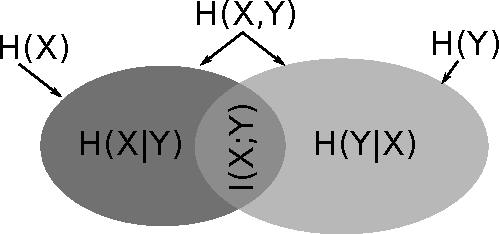
\includegraphics[width=\linewidth]{figures/info-set.pdf}
  \caption{Diagrama de Venn ilustrando as relações entre entropias, entropias condicionais e informação mútua, facilitando a visualização das grandezas informacionais.}
  \label{fig:vennshannon}
\end{marginfigure}

De forma semelhante que vimos anteriormente, quando foi introduzido
o conceito de entropia condicional, podemos agora estender o conceito
de informação mútua entre duas variáveis aleatórias $X$ e $Y$ dado o 
conhecimento de uma terceira variável $Z$, definindo assim a informação 
mútua condicional.
\begin{definition}[Informação Mútua Condicional]\label{def:infmutcond}
Dadas as variáveis aleatórias $X$, $Y$ e $Z$, a informação mútua entre
$X$ e $Y$, condicionada ao conhecimento de $Z$ é dada por
\begin{subequations}\label{eq:mutinfcond}
{
\allowdisplaybreaks
\begin{align}
I(X;Y|Z) &\triangleq \sum_z p(z) I(X;Y|Z=z) \\
         &= \sum_z p(z) E_{p(x,y|z)} \log \frac{p(x,y|Z=z)}{p(x|Z=z) p(y|Z=z)} \\
         &= \sum_{x,y,z} p(x,y,z) \log \frac{p(x,y|z)}{p(x|z)p(y|z)} \\
	 &= \sum_{x,y,z} p(x,y,z) \log \frac{p(x|y,z)p(y|z)}{p(x|z)p(y|z)} \\
	 &= \E_{p(x,y,z)} \left[ \log \frac{1}{p(x|z)} - \log \frac{1}{p(x|y,z)} \right] \\
         &= H(X|Z) - H(X|Y,Z) .
\end{align}
}
\end{subequations}
\end{definition}





\section{Generalização da Regra da Cadeia}\label{sec-genchainrule}

A generalização é fundamental para analisar sistemas com múltiplas variáveis ou séries temporais.
Uma sequência de variáveis aleatórias $X_1, X_2, \ldots, X_N = X_{1:N}$ pode representar estados ou observações ao longo do tempo.
A regra da cadeira, vista anteriormente no \Cref{thm:regracadeia},
pode ser generalizada para uma sequência de $N$ variáveis aleatórias $X_{1:N}$.

\begin{proposition}[Regra da Cadeia Generalizada da Entropia]\label{prop:regracadeiagen}
Dada uma sequência de $N$ variáveis aleatórias $X_{1:N}$, a entropia conjunta pode ser dada por 
\begin{equation}\label{eq:regracadeiagen}
H(X_1, X_2, \ldots, X_N) = \sum_{i=1}^{N} H(X_i|X_1, \ldots, X_{i-1}) .
\end{equation}
\end{proposition}
\begin{proof}
A demonstração é feita por indução. Sabemos que para $N=2$ é verdadeiro, como visto no \Cref{thm:regracadeia}.
Vamos supor que para $N=M$ é verdadeiro e mostrar que para $N=M+1$ é verdadeiro.
\begin{subequations}\label{eq:dmgenregracadeia}
\begin{align}
    H(X_1, X_2, \ldots, X_M, X_{M+1}) &= H(X_1, X_2, \ldots, X_M) + H(X_{M+1} | X_1, X_2, \ldots, X_M) \label{eq:dmgenregracadeia1}\\
				      &= \sum_{i=1}^{M} H(X_i|X_1, \ldots, X_{i-1}) + H(X_{M+1} | X_1, X_2, \ldots, X_M) \label{eq:dmgenregracadeia2}\\
 &= \sum_{i=1}^{M+1} H(X_i|X_1, \ldots, X_{i-1}) ,
\end{align}
\end{subequations}
onde em \ref{eq:dmgenregracadeia1} utilizamos o \Cref{thm:regracadeia}, fazendo $X=(X_1, X_2, \ldots, X_M)$ e $Y=X_{M+1}$,
e em \ref{eq:dmgenregracadeia2} utilizamos a premissa de que a relação \ref{eq:regracadeiagen} é válida para $N=M$.
Isto prova então que a relação \ref{eq:regracadeiagen} é válida para $N=M+1$ e, como é sabidamente válida para $N=2$,
será válida para todo $N$.
\end{proof}


A regra da cadeia vista no \Cref{thm:regracadeia} pode ser estendida para o caso do condicionamento
à uma terceira variável aleatória.
\begin{proposition}[Regra da Cadeia Condicional]\label{pro:regracadeiacond}
Para duas variáveis aleatórias  $X$ e $Y$ condicionadas a uma terceira, $Z$, 
a entropia conjunta condicional pode ser decomposta como:
\begin{equation}\label{eq:regracadeiacond}
    H(X,Y|Z) \: = H(X|Z) + H(Y|X,Z) .
\end{equation}
A incerteza total sobre $(X,Y)$, dado $Z$, pode ser quebrada em duas partes: 
primeiro, a incerteza sobre $X$ dado $Z$, e depois a incerteza adicional de $Y$ 
dado tanto $X$ quanto $Z$. 
\end{proposition}
\begin{proof}
A demonstração segue os mesmos passos da demonstração do \Cref{thm:regracadeia}, bastando
condicionar a $Z$ para obtermos a adaptação para a regra da cadeia condicional.
\end{proof}


Fazemos agora a generalização para uma sequência de variáveis aleatórias $X_{1:N}$ 
condicionada a uma variável aleatória $Y$.
\begin{proposition}[Regra da Cadeia Condicional Generalizada]\label{pro:regracadeiacondgen}
\begin{equation}\label{eq:regracadeiacondgen}
H(X_1, X_2, \ldots, X_N | Y) = \sum_{i=1}^{N} H(X_i|X_1, \ldots, X_{i-1}, Y) .
\end{equation}
\end{proposition}
\begin{proof}
\begin{subequations}\label{eq:dmgenregracadeiagen}
\begin{align}
    H(X_1, X_2, \ldots, X_N | Y) &= \sum_y H(X_1, X_2, \ldots, X_N | Y = y) \label{eq:dmgenregracadeiagen1}\\
				 &= \sum_y p(y) \sum_{i=1}^{N} H(X_i|X_1, \ldots, X_{i-1}, Y=y) \label{eq:dmgenregracadeiagen2}\\
				 &= \sum_{i=1}^{N} \sum_y p(y) H(X_i|X_1, \ldots, X_{i-1}, Y=y) \label{eq:dmgenregracadeiagen3}\\
				 &= \sum_{i=1}^{N} H(X_i|X_1, \ldots, X_{i-1}, Y) ,\label{eq:dmgenregracadeiagen4}
\end{align}
\end{subequations}
onde utilizamos \ref{eq:entcondevents} em \ref{eq:dmgenregracadeiagen1},
\ref{eq:entcondeventsZ} em \ref{eq:dmgenregracadeiagen4}, e
\ref{eq:dmgenregracadeiagen2} segue de \ref{eq:regracadeiagen}.
\end{proof}

Por fim, podemos aplicar as mesmas ideias para obter a regra da cadeia para
informação mútua, que descreve como a informação compartilhada entre um
conjunto de variáveis e outra variável pode ser decomposta em contribuições
condicionais. 
\begin{proposition}[Regra da Cadeia da Informação Mútua]\label{pro:regracadeiainfmut}
\begin{equation}\label{eq:regracadeiainfmut}
I(X_1, X_2, \ldots, X_N ; Y) = \sum_{i=1}^{N} I(X_i;Y|X_1, \ldots, X_{i-1}) .
\end{equation}
\end{proposition}
\begin{proof}
\begin{subequations}\label{eq:dmregracadeiainfmut}
\begin{align}
    I(X_1, X_2, \ldots, X_N ; Y) &= H(X_1, X_2, \ldots, X_N) - H(X_1, X_2, \ldots, X_N | Y) \\
				 &= \sum_{i=1}^{N} \left[ H(X_i | X_1, \ldots, X_{i-1}) - H(X_i | X_1, \ldots, X_{i-1}, Y) \right] \\
				 &= \sum_{i=1}^{N} I(X_i;Y|X_1, \ldots, X_{i-1}) ,
\end{align}
\end{subequations}
onde utilizamos as \Cref{prop:regracadeiagen,pro:regracadeiacondgen}.
\end{proof}





\section{Desigualdade de Jensen}\label{sec:desjensen}
Nesta seção, apresentamos a desigualdade de Jensen, uma relação observada para
funções convexas entre o valor esperado da função de uma variável
aleatória e a função do valor esperado desta variável aleatória. Mais precisamente,
$\E f(X) \geq f(\E X)$, para $f$ uma função convexa e $X$ uma variável aleatória.

A desigualdade de Jensen é uma ferramenta fundamental para demonstrar diversas propriedades essenciais.
Entretanto, primeiramente devemos rever o teste da segunda derivada para convexidade.

\begin{definition}[Função Convexa]
Dizemos que $f$ é convexa em $(a,b)$ se para todo $x_1,x_2 \in (a,b)$, $0 \leq \lambda \leq 1$,
\begin{equation}
f(\lambda x_1 + (1 - \lambda)x_2) \leq \lambda f(x_1) + (1-\lambda) f(x_2)
\end{equation}
\end{definition}

A \Cref{fig:funcao-convexa} ilustra uma função convexa no intervalo, evidenciando
como a imagem de um ponto intermediário $\lambda x_1 + (1 - \lambda)x_2$, entre
$x_1$ e $x_2$, é menor ou igual ao correspondente na corda que passa por $(x_1,f(x_1))$
e $(x_2,f(x_2))$.

\begin{marginfigure}%
  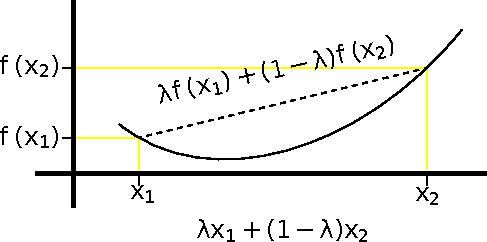
\includegraphics[width=\linewidth]{figures/funcao-convexa.pdf}
  \caption{Ilustração de uma função convexa no intervalo.}
  \label{fig:funcao-convexa}
\end{marginfigure}

Alguns exemplos de funções convexas são: $f(x)=x^2$; $f(x)=x^4$; $f(x)=e^x$; e $x \log x$, $x \geq 0$.
Teremos que $f$ é estritamente convexa se a igualdade for verdadeira apenas para $\lambda = 0$ ou $\lambda = 1$.
Uma função $f$ é dita côncava se $-f$ ($f$ multiplicada por $-1$) for uma função convexa, ou seja,
côncavo é o oposto de convexo.

Para determinar se uma função é convexa, podemos realizar o simples teste da segunda derivada.


\begin{proposition}[Teste da Segunda Derivada para Convexidade]
Se uma função $f$ possui derivada segunda não-negativa (positiva) em um intervalo,
a função é convexa (estritamente convexa) no intervalo.
\end{proposition}
\begin{proof}
  A expansão de Taylor de uma função $f$ em torno do ponto $x_0$ é dada por
  \begin{equation}
  f(x) = f(x_0) + f'(x_0) (x-x_0) + \frac{f''(x^\ast)}{2} (x-x_0)^2
  \end{equation}
  onde $x^\ast \in (x_0,x)$. Por hipótese, $f''(x^\ast) \geq 0$, e desta forma,
  o último termo é não-negativo.

  Seja $x_0 = \lambda x_1 + (1-\lambda) x_2$. Analisando em $x=x_1$, teremos
  \begin{subequations}\label{eq:dmtestsecderv1}
  \begin{align}
    f(x_1) &\geq f(x_0) + f'(x_0) (x_1 - \lambda x_1 - (1-\lambda)x_2) \label{eq:dmtestsecderv1-1}\\
	   &= f(x_0) + f'(x_0) ((1-\lambda)(x_1-x_2)) \label{eq:dmtestsecderv1-2}
  \end{align}
  \end{subequations}
  Da mesma forma, em $x=x_2$, teremos
  \begin{subequations}\label{eq:dmtestsecderv2}
  \begin{align}
    f(x_2) &\geq f(x_0) + f'(x_0) (x_2 - \lambda x_1 - (1-\lambda)x_2) \label{eq:dmtestsecderv2-1}\\
           &= f(x_0) + f'(x_0) (\lambda(x_2-x_1)) \label{eq:dmtestsecderv2-2}
  \end{align}
  \end{subequations}

  Somando $\lambda$ \ref{eq:dmtestsecderv1-2} com $(1-\lambda)$ \ref{eq:dmtestsecderv2-2}, obtemos
  \begin{subequations}\label{eq:dmtestsecderv3}
  \begin{align}
  \lambda f(x_1) + (1-\lambda) f(x_2) &\geq \lambda f(x_0) + \lambda f'(x_0) ((1-\lambda)(x_1-x_2)) + (1-\lambda) f(x_0) + (1-\lambda) f'(x_0) (\lambda(x_2-x_1)) \\
        &\geq f(x_0) = f(\lambda x_1 + (1-\lambda) x_2)
  \end{align}
  \end{subequations}
\end{proof}



Podemos agora retornar à desigualdade de Jensen. Vemos na \Cref{fig:jensen} uma ilustração
do que tal propriedade representar.
\begin{marginfigure}%
  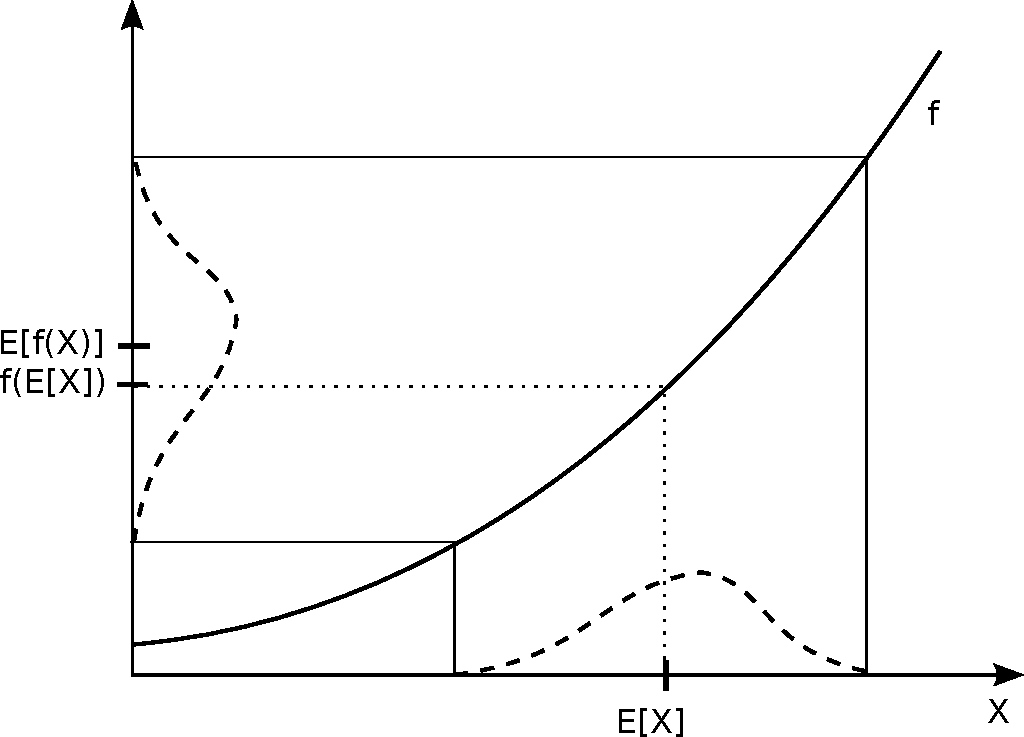
\includegraphics[width=\linewidth]{figures/jensen.pdf}
  \caption{Ilustração da desigualdade de Jensen, fornecendo uma intuição para ela.}
  \label{fig:jensen}
\end{marginfigure}


\begin{theorem}[Desigualdade de Jensen]\label{thm-desjensen}
Seja $f$ uma função convexa e $X$ uma variável aleatória, então
\begin{equation}\label{eq:desjensen}
\E f(X) \: = \sum_x p(x) f(x) \geq f(\E X) \: = f \left( \sum_x x p(x) \right)
\end{equation}
\end{theorem}
\begin{proof}
Para uma distribuição de massa com apenas dois pontos
\begin{equation}
\E[f(X)] \: = p_1 f(x_1) + p_2 f(x_2) \geq f(p_1 x_1 + p_2 x_2) = f(\E X)
\end{equation}
já que $f$ é convexa e $p_1+p_2=1$.

Para uma distribuição com mais de dois ponto, iremos fazer uma demonstração
por indução.

Suponha que o teorema seja verdadeiro para uma distribuição com $k-1$ pontos de massa.
Para uma distribuição com $k$ pontos de massa podemos escrever cada
$p_i' = p_i / (1-p_k)$ para $i=1,2,\ldots,k-1$.

Desta forma, teremos
\begin{subequations}\label{dem:jensen}
\begin{align}
\E[f(X)] &= \sum_{i=1}^k p_i f(x_i) \label{dem:jensen1}\\
         &= \sum_{i=1}^{k-1} (1-p_k)p_i' f(x_i) + p_k f(x_k) \label{dem:jensen2}\\
         &= (1-p_k) \sum_{i=1}^{k-1} p_i' f(x_i) + p_k f(x_k) \label{dem:jensen3}\\
	 &\geq (1-p_k) f\left( \sum_{i=1}^{k-1} p_i' x_i \right) + p_k f(x_k) \label{dem:jensen4}\\
	 &\geq f \left( (1-p_k) \sum_{i=1}^{k-1} p_i' x_i + p_k x_k \right) \\
	 &= f\left( \sum_{i=1}^{k} p_i x_i \right)
\end{align}
\end{subequations}
onde em \ref{dem:jensen3} utilizamos a hipótese de indução, já que
\begin{equation}
\sum_{i=1}^{k-1} p_i' = \sum_{i=1}^{k-1} \frac{p_i}{1-p_k} = \frac{1-p_k}{1-p_k} = 1 .
\end{equation}
e em \ref{dem:jensen4} utilizamos a definição de convexidade.

Desta forma, sendo o teorema válido para uma distribuição de massa com $k-1$ pontos,
também será verdadeiro para uma distribuição de massa com $k$ pontos.
Como mostramos que para $k=2$ é verdadeiro, logo o teorema é verdadeiro para qualquer $k$.
\end{proof}


A desigualdade de Jensen pode ser utilizada para demonstrar a não negatividade
da divergência de KL.
\begin{lemma}[Não negatividade da Divergência de Kullback–Leibler]
\begin{equation}
D(p||q) \geq 0 \text{ com igualdade se e somente se } p(x) = q(x) \forall x.
\end{equation}
\end{lemma}
\begin{proof}
De forma equivalente, iremos mostrar que $-D(p||q) \leq 0$.

Seja $S_p=\{x: p(x) > 0\}$, o suporte de $p$, então
\begin{subequations}\label{dem:divnonneg}
\begin{align}
-D(p||q) &= -\sum_x p(x) \log \frac{p(x)}{q(x)} = -\sum_{x \in S_p} p(x) \log \frac{p(x)}{q(x)} \label{dem:divnonneg1}\\
         &= \sum_{x \in S_p} p(x) \log \frac{q(x)}{p(x)} = \E \log \frac{q(X)}{p(X)} \label{dem:divnonneg2}\\
	 &\leq \log \left( E \frac{q(X)}{p(X)} \right) = \log \left( \sum_{x \in S_p} p(x) \frac{q(x)}{p(x)} \right) \label{dem:divnonneg3}\\
	 &= \log \left( \sum_{x \in S_p} q(x) \right) \leq \log \left( \sum_x  q(x) \right) = \log 1 = 0 \label{dem:divnonneg4}
\end{align}
\end{subequations}
onde em \ref{dem:divnonneg2} utilizamos a desigualdade de Jensen, \Cref{eq:desjensen}.
\end{proof}



A desigualdade da soma dos logaritmos é derivada da desigualdade de Jensen e da convexidade da função logarítmica.
Esta desigualdade também aparece em algumas demonstrações importantes.

\begin{proposition}[Desigualdade da Soma de Logaritmos]
Dados $(a_1, \ldots, a_n)$ e $(b_1,\ldots,b_n)$, com $a_i \geq 0$ e $b_i \geq 0$, temos
\begin{equation}\label{eq:dessomalog}
\sum_{i=1}^n a_i \log \frac{a_i}{b_i} \geq \left( \sum_{i=1}^n a_i \right) \log \frac{\sum_{i=1}^n a_i}{\sum_{i=1}^n b_i}
\end{equation}
e teremos igualdade se e somente se $a_i/b_i = c$, onde $c$ é uma constante.
\end{proposition}
\begin{proof}
Considere $f(t) = t \log t = t (\ln t) (\log e)$, que é estritamente convexa, pois
$f''(t) = 1/t \log e >0$, $\forall t > 0$.

Dada $f$ convexa, a desigualdade de Jensen diz que
\begin{equation}
\sum_i \alpha_i f(t_i) \geq f \left( \sum_i \alpha_i t_i \right) \text{ com } \alpha_i \geq 0 \text{ e } \sum_i \alpha_i = 1.
\end{equation}
$f(x) = x \log x$ é estritamente convexa para $x>0$, já que $f''(x)=\frac{1}{x} \log e > 0$ para $x>0$.

Vamos fazer $\alpha_i = \sfrac{b_i}{\sum_{j=1}^n b_j}$ e $t_i = \sfrac{a_i}{b_i}$, então obteremos
\begin{subequations}
    \begin{align}
	\sum_i \alpha_i f(t_i) &\geq f \left( \sum_i \alpha_i t_i \right) \\
	\sum_i \left( \frac{b_i}{\sum_j b_j} f \left( \frac{a_i}{b_i} \right) \right) &\geq f \left( \sum_i \frac{b_i}{\sum_j b_j} \frac{a_i}{b_i} \right) \\
	\frac{1}{\sum_j b_j} \sum_i \left( b_i \frac{a_i}{b_i} \log \frac{a_i}{b_i} \right) &\geq \left( \sum_i \frac{a_i}{\sum_j b_j} \right) \log \sum_i \frac{a_i}{\sum_j b_j} \\
	\sum_i a_i \log \frac{a_i}{b_i} &\geq \left( \sum_i a_i \right) \log \sum_i \frac{a_i}{\sum_j b_j} \\
	\sum_i a_i \log \frac{a_i}{b_i} &\geq \sum_i a_i \log \frac{\sum_i a_i}{\sum_j b_j} .
    \end{align}
\end{subequations}
\end{proof}

A desigualdade da soma de logaritmos pode ser utilizada para mostrar que $D(p||q) \geq 0$.
\begin{proposition}[Não negatividade da Divergência]
$D(p||q) \geq 0$
\end{proposition}
\begin{proof}
  \begin{subequations}
  \begin{align}
  D(p||q) &= \sum_x p(x) \log \frac{p(x)}{q(x)} \\
          &\geq \left( \sum_x p(x) \right) \log \frac{\sum_x p(x)}{\sum_x q(x)} \\
          &= 1 \log \frac{1}{1} = 0 .
  \end{align}
  \end{subequations}
\end{proof}


A entropia relativa, ou divergência de Kullback-Leibler, possui uma propriedade importante: ela é convexa no par de distribuições.
A convexidade no par considera a interpolação simultânea de ambas as distribuições e garante que a divergência KL se comporte de forma previsível ao combinar distribuições.

\begin{theorem}[A Entropia Relativa é Convexa no Par]
Para dois pares de distribuições $(p_1, q_1)$ e $(p_2, q_2)$, 
\begin{equation}\label{eq:entrelconvpar}
D(\lambda p_1 + (1 - \lambda) p_2 || \lambda q_1 + (1- \lambda)q_2) \leq \lambda D(p_1 || q_1) + (1- \lambda) D(p_2 || q_2) ,
\end{equation}
para todo $0 \leq \lambda \leq 1$.
\end{theorem}
\begin{proof}
Usando a \Cref{def:divKL}, definição de divergência de KL, temos
\begin{subequations}\label{dem:entrelconvpar}
\begin{align}
    D(\lambda p_1 + (1 - \lambda) p_2 || \lambda q_1 + (1- \lambda)q_2) &= \sum_x (\lambda p_1(x) + (1 - \lambda) p_2(x) ) \log \frac{\lambda p_1(x) + (1 - \lambda) p_2(x)}{\lambda q_1(x) + (1 - \lambda) q_2(x)} \label{dem:entrelconvpar1} \\
									&\leq \sum_x \left( \lambda p_1(x) \log \frac{\lambda p_1(x)}{\lambda q_1(x)} + (1 - \lambda) p_2(x) \log \frac{(1 - \lambda) p_2(x)}{(1-\lambda) q_2(x)} \right) \label{dem:entrelconvpar2} \\
									&= \lambda D(p_1 || q_1) + (1 - \lambda) D(p_2 || q_2) \label{dem:entrelconvpar3}
\end{align}
\end{subequations}
onde, em \ref{dem:entrelconvpar1}, podemos considerar que, dentro do somatório em $x$, temos um somatório com dois termos: $(a_1+a_2) \log \left( \sfrac{(a_1+a_2)}{(b_1 + b_2)} \right)$.
Utilizamos então a \Cref{eq:dessomalog} para o caso com apenas dois temos:
\begin{equation}
\left( \sum_{i=1}^2 a_i \right) \log \frac{\sum_{i=1}^2 a_i}{\sum_{i=1}^{2} b_i} \leq \sum_{i=1}^2 a_i \log \frac{a_i}{b_i} =  a_1 \log \frac{a_1}{b_1} + a_2 \log \frac{a_2}{b_2},
\end{equation}
o que nos leva ao resultado em \ref{dem:entrelconvpar2}. E usamos novamente a \Cref{def:divKL} para obter \ref{dem:entrelconvpar3}.
\end{proof}




\begin{theorem}[A Entropia Relativa é Convexa no Primeiro Argumento]\label{thm:divklconvp}
A divergência de Kullback-Leibler, $D(p||q)$, é convexa em relação a $p$, fixando-se $q$.
Ou seja, dadas $p_1$ e $p_2$, duas distribuições de probabilidade, e fixando-se $q$,
a distribuição de referência ou distribuição base. Temos então, para $\lambda \in [0,1]$,
\begin{equation}
D(\lambda p_1+(1-\lambda)p_2|q) \leq D(p_1|q) + (1-\lambda)D(p_2|q) .
\end{equation}
\end{theorem}
\begin{proof}
\begin{subequations}\label{dem:divklconv}
\begin{align}
D(\lambda p_1+(1-\lambda)p_2|q) &= \sum_x \left(\lambda p_1+(1-\lambda)p_2\right)\log\frac{\lambda p_1+(1-\lambda)p_2}{q} \label{dem:divklconv1}\\
				&\leq \lambda \sum_x p_1 \log \frac{p_1}{q} + (1-\lambda) \sum_x p_2 \log \frac{p_2}{q} \label{dem:divklconv2}\\
				&= \lambda D(p_1||q) + (1-\lambda) D(p_2||q) ,\label{dem:divklconv3}
\end{align}
\end{subequations}
onde em \ref{dem:divklconv1} utilizamos que a função $f(p) = p \log p$ é convexa em $p$ 
(lembrando que $q$ é fixo e assim $f''(p) = \sfrac{1}{p} > 0$, para $p>0$) e utilizando
a desigualdade de Jensen (\Cref{thm-desjensen}). Em \ref{dem:divklconv2} apenas utilizamos a
definição de divergência (\Cref{def:divKL}).
\end{proof}
A entropia relativa, entretanto, não é convexa no segundo argumento. Será entretanto
côncava em $q$ para $p$ fixo. A demonstração deixamos a cargo do leitor.

O \Cref{thm:divklconvp} pode ser utilizado para demonstrar a concavidade da entropia.
\begin{theorem}[A Entropia é Côncava]\label{thm:entropiaconcava}
$H(p)$ é uma função concava de $p$.
\end{theorem}
\begin{proof}
\begin{subequations}\label{dem:entropiaconcava}
\begin{align}
    H(p) &= - \sum_i p_i \log p_i = - \sum_i p_i \log p_i  + \log \vert \mathcal{X} \vert - \log \vert \mathcal{X} \vert \label{dem:entropiaconcava1}\\
        &= \log \vert \mathcal{X} \vert - \sum_i p_i \log p_i - \log \vert \mathcal{X} \vert \underbrace{\sum_i p_i}_{=1} \label{dem:entropiaconcava2}\\
        &= \log \vert \mathcal{X} \vert - \sum_i \left( p_i \log p_i + p_i \log \vert \mathcal{X} \vert \right) \label{dem:entropiaconcava3}\\
        &= \log \vert \mathcal{X} \vert - \sum_i p_i \left( \log p_i -  \log \sfrac{1}{\vert \mathcal{X} \vert } \right) \label{dem:entropiaconcava4}\\
        &= \underbrace{\log \vert \mathcal{X} \vert}_{\text{constante}} - \underbrace{D(p||u)}_{\text{convexo}} \label{dem:entropiaconcava5}
\end{align}
\end{subequations}
\end{proof}
A partir da relação em \ref{dem:entropiaconcava5}, podemos ver a entropia como a similaridade com a distribuição uniforme.
Quanto maior a entropia (menor a divergência $D(p||u)$), mais próximo estaremos da distribuição uniforme.


Analisaremos agora a convexidade ou concavidade da informação mútua $I(X;Y)$, quando fixamos uma das distribuições condicionais ou marginais.
Essa análise possui implicação direta na determinação da capacidade de canal em teoria da comunicação, onde a maximização da informação mútua,
sobre a distribuição de entrada, será um problema bem comportado com um único máximo global. A concavidade da função objetivo
implica que o máximo é atingível e pode ser encontrado usando técnicas de otimização convexa.

\begin{theorem}[Concavidade/Convexidade da Informação Mútua]\label{thm:concconvinfmut}
Seja $(X,Y) \sim p(x,y) = p(x)p(y|x)$, a informação mútua $I(X;Y)$ é uma função côncava
de $p(x)$ para $p(y|x)$ fixo e uma função convexa de $p(y|x)$ para $p(x)$ fixo.
\end{theorem}
\begin{proof}
Vejamos primeiro o motivo de $I(X;Y)$ ser uma função côncava de $p(x)$ para $p(y|x)$ fixo.
Podemos escrever a informação mútua como uma função de $p(x)$:
\begin{subequations}\label{dem:concconvinfmutA}
\begin{align}
    I(X;Y) &= D(p(x,y)||p(x)p(y)) \label{dem:concconvinfmutA1} \\
       &= \sum_{x,y} p(x,y) \log \frac{p(x,y)}{p(x)p(y)} \label{dem:concconvinfmutA2}\\
       &=& \sum_{x,y} p(x)p(y|x) \log \frac{ p(x)p(y|x) }{p(x) \sum_x p(x) p(y|x)}, \label{dem:concconvinfmutA3}
\end{align}
\end{subequations}
onde em \ref{dem:concconvinfmutA1} utilizamos a definição de informação mútua, 
em \ref{dem:concconvinfmutA2} utilizamos a definição de divergência e aplicamos o teorema de Bayes em \ref{dem:concconvinfmutA3}.
Se $p(y|x)$ é constante, então a informação mútua é função de $p(x)$: $I_{p(x)} (X;Y)$.
Utilizando a propriedade da convexidade da divergência de Kullback-Leibler,
\begin{equation}\label{eq-Imixpx}
I_{\lambda p_1(x) + (1-\lambda)p_2(x)} (X;Y) \geq \lambda I_{p_1(x)} (X;Y) + (1-\lambda) I_{p_2(x)} (X;Y) .
\end{equation}
Então a informação mútua é uma função concava de $p(x)$ para $p(y|x)$ fixo.

Agora iremos demonstrar que $I(X;Y)$ é uma função convexa de $p(y|x)$ para $p(x)$ fixo.
Aplicamos a mesma ideia, porém agora consideraremos $p(x)$ fixo. Escrevemos então a informação mútua como uma função de $p(y|x)$:
\begin{equation}
I_{p(y|x)} (X;Y) = \sum_{x,y} p(x) p(y|x) \log \frac{p(x) p(y|x)}{p(x) \sum_x p(x) p(y|x)} .
\end{equation}
Utilizando a propriedade da convexidade da divergência de Kullback-Leibler, obtemos
\begin{equation}\label{eq-Imixpxy}
I_{\lambda p_1(y|x) + (1-\lambda)p_2(y|x)} (X;Y) \leq \lambda I_{p_1(y|x)} (X;Y) + (1-\lambda) I_{p_2(y|x)} (X;Y) .
\end{equation}
\end{proof}




\section{Desigualdade de Processamento de Dados}
Quando falamos em processamento de dados, podemos pensar no seguinte modelo:
$X \rightarrow Y \rightarrow Z$, onde a variável aleatória $X$ representa
os dados originais, a serem transmitidos; $Y$ representa os dados recebidos no outro lado de um canal 
de comunicação; e $Z$ o resultado de um processamento adicional aplicado a $Y$.
O processamento de dados é modelado como uma cadeia de Markov.
Nessa estrutura, $Z$ depende de $X$ apenas através de $Y$,
ou, de outra forma, $Z$ e $X$ são condicionalmente independentes, dado $Y$.


\begin{definition}[Cadeia de Markov]\label{def:markovchain}
As variáveis aleatórias $X$, $Y$ e $Z$ formam uma cadeia de Markov nesta ordem
(denotado $X \rightarrow Y \rightarrow Z$) se a distribuição condicional de $Z$
depende apenas de $Y$ e é condicionalmente independente de $X$. Especificamente,
$X$, $Y$ e $Z$ formam uma cadeia de Markov $X \rightarrow Y \rightarrow Z$ se
a função massa de probabilidade conjunta pode ser escrita como
\begin{equation}\label{eq:markov}
p(x,y,z) = p(x) p(y|x) p(z|y)
\end{equation}
\end{definition}

Temos uma cadeia de Markov $X \rightarrow Y \rightarrow Z$ se, e somente se,
$X$ e $Z$ são condicionalmente independentes dado $Y$ ($X \independent Z | Y$).
Isto é,
\begin{equation}
p(x,z|y) = \frac{p(x,y,z)}{p(y)} = \frac{p(x)p(y|x)p(z|y)}{p(y)} = p(x|y) p(z|y) \ \ \forall x,y,z
\end{equation}

\begin{proposition}[Cadeia de Markov Inversa]\label{prop:markovinv}
Se $X$, $Y$ e $Z$ formam uma cadeia de Markov nesta ordem ($X \rightarrow Y \rightarrow Z$), então
também formam uma cadeia de Markov na ordem inversa ($Z \rightarrow Y \rightarrow X$).
\end{proposition}
\begin{proof}
\begin{subequations}\label{dem:markovinv}
\begin{align}
p(x,y,z) &= p(x)p(y|x)p(z|y) = p(x,y)p(z|y) \\
         &= \frac{p(x,y)p(z|y)p(y)}{p(y)} = p(x|y) p(y,z) \\
         &= p(x|y) p(y|z) p(z)
\end{align}
\end{subequations}
\end{proof}

A Desigualdade do Processamento de Dados estabelece que a informação mútua
entre variáveis aleatórias não aumenta sob o processamento de dados. Em outras
palavras, a informação relevante para uma variável não pode ser aumentada ao
processar outra variável relacionada em uma cadeia de Markov.
\begin{theorem}[Desigualdade do Processamento de Dados]\label{thm:desgprocdados}
Se $X \rightarrow Y \rightarrow Z$ então
\begin{equation}\label{eq:desgprocdados}
I(X;Y) \geq I(X;Z)
\end{equation}
\end{theorem}
\begin{proof}
Utilizando a regra da cadeia da informação mútua (\Cref{pro:regracadeiainfmut}), teremos
\begin{subequations}\label{dem:desgprocdadosA}
  \begin{align}
    I(X;Y,Z) &= I(X;Z) + I(X;Y|Z) \label{dem:desgprocdadosA1}\\
             &= I(X;Y) + I(X;Z|Y) \label{dem:desgprocdadosA2}
  \end{align}
\end{subequations}
Como $X \independent Z |Y$ ($X$ e $Z$ são condicionalmente independentes, dado $Y$), temos
que $I(X;Z|Y)=0$. Como $I(X;Y|Z) \geq 0$, usando \cref{dem:desgprocdadosA1,dem:desgprocdadosA2}, teremos
\begin{equation}
I(X;Z) + \underbrace{I(X; Y|Z)}_{\geq 0} = I(X;Y) + \bcancelto{0}{I(X;Z|Y)} ,
\end{equation}
Podemos conclui então que
\begin{equation}
I(X;Z) \leq I(X;Y) .
\end{equation}
\end{proof}
Note que teremos igualdade na \Cref{eq:desgprocdados} se, e somente se, $I(X;Y|Z)=0$ (i.e. $X \rightarrow Z \rightarrow Y$).
De forma similar, também podemos mostrar que $I(Y;Z) \geq I(X;Z)$.

\begin{corollary}
Se $Z=g(Y)$, então $I(X;Y) \geq I(X;g(Y))$.
\end{corollary}
\begin{proof}
$X \rightarrow Y \rightarrow g(Y)$ forma uma cadeia de Markov.
\end{proof}

\begin{corollary}\label{col:infmutxyzleq}
Se $X \rightarrow Y \rightarrow Z$ então $I(X;Y|Z) \leq I(X;Y)$.
\end{corollary}
\begin{proof}
\begin{equation}
\underbrace{I(X;Z)}_{\geq 0} + I(X; Y|Z) = I(X;Y) + \bcancelto{0}{I(X;Z|Y)}
\end{equation}
então
\begin{equation}
I(X; Y|Z) \leq I(X;Y).
\end{equation}
\end{proof}

Note também que
\begin{subequations}
  \begin{align}
    I(X; Y|Z) &= H(X|Z) - H(X|Y,Z) \\
              &\leq H(X) - H(X|Y) \\
              &= I(X;Y) .
  \end{align}
\end{subequations}

O processamento digital de imagem para remoção de ruído, por exemplo, é uma
aplicação prática para a desigualdade de processamento de dados. Considere $X$
como a imagem original, $Y$ como a imagem ruidosa recebida em uma comunicação,
e $Z$  a imagem após o processamento para remoção de ruído. Podemos considerar
que temos aqui uma cadeia de Markov $X \rightarrow Y \rightarrow Z$ e assim
podemos aplicar a desigualdade de processamento de dados, que nos diz:
$I(X;Z) \leq I(X;Y)$. O processo de remoção de ruído não pode aumentar a informação
mútua entre a imagem original $X$ e a imagem processada $Z$ além do que já
existe entre $X$ e $Y$, indicando uma perda inevitável de informação devido ao
ruído. No entanto, a remoção de ruído é possível porque o algoritmo pode
explorar regularidades estatísticas ou estruturais na imagem.




\section{Algumas Relações Notáveis}

\begin{proposition}[Determinismo e a incerteza nula]\label{prop:detincertnull}
$H(X)=0$ se, e somente se, $X$ for determinístico.
\end{proposition}
\begin{proof}
Se $X$ é determinístico, então existe $x^\ast \in \mathcal{X}$ tal que $p(x^\ast) = 1$ e
$p(x) = 0 \forall x \neq x^\ast$. Neste caso, teremos $H(X) = -p(x^\ast) \log p(x^\ast) = 0$.
Por outro lado, se $X$ não for determinístico, então existe $x^\ast \in \mathcal{X}$ tal que $0 < p(x^\ast) < 1$.
Desta forma, $H(X) \geq -p(x^\ast) \log p(x^\ast) \geq 0$. Podemos concluir assim que
$H(X) = 0$ se e somente se $X$ for determinístico.
\end{proof}


\begin{proposition}[Quando $Y$ é uma função de $X$]
$H(Y|X) = 0$ se, e somente se, $Y$ for um função de $X$, ou seja, $Y = g(X)$.
\end{proposition}
\begin{proof}
  Observando a \Cref{eq:entcondevents}, podemos concluir que $H(Y|X) = 0$
  se e somente se todos os termos do somatório forem nulos, ou seja,
  $H(Y|X = x) = 0$ para cada $x \in S_X$.
  A partir da \Cref{prop:detincertnull}, sabemos que isto ocorre se, e somente se,
  $Y$ é determinístico para cada $x$ dado. Em outras palavras, $Y$ é uma função de $X$.
\end{proof}
\begin{proof}
  Uma outra forma de demonstração é por contradição. Assuma que existe $x$, digamos $x_0$, e dois valores diferentes de $y$, digamos $y_1$ e $y_2$,
  tal que $p(x_0,y_1) > 0$ e $p(x_0,y_2)>0$. Então a marginal é $p(x_0) \geq p(x_0,y_1) + p(x_0,y_2) > 0$.
  Temos também
  \begin{equation}
  p(y_1|x_0) = \frac{p(x_0,y_1)}{p(x_0)} \text{ e } p(y_2|x_0) = \frac{p(x_0,y_2)}{p(x_0)}
  \end{equation}
  então ambos $p(y_1|x_0)$ e $p(y_2|x_0)$ não são iguais a $0$ (zero) ou $1$ (um).

  \begin{subequations}
    \begin{align}
      H(Y|X) &= E[H(Y|X)] \\
        &= - \sum_x p(x) H(Y|X=x) \\
        &= - \sum_x p(x) \sum_y p(y|x) \log p(y|x) \\
        &\geq - p(x_0) \sum_y p(y|x_0) \log p(y|x_0) \\
        &\geq - \underbrace{p(x_0)}_{>0} [ \underbrace{p(y_1|x_0)}_{>0} \underbrace{\log p(y_1|x_0)}_{<0} + \underbrace{p(y_2|x_0)}_{>0} \underbrace{\log p(y_2|x_0)}_{<0} ]  \\
        &> 0
    \end{align}
  \end{subequations}

  Então, a entropia condicional $H(Y|X)$ é nula se e somente se $Y$ for uma função de $X$.
  Se $Y$ for uma função de $X$, teremos $p(y_1|x_0) = 0 \text{ ou } 1$, ou seja, a probabilidade
  $p(y_i|x_0)$ será igual a $1$ apenas para um $y_i$ e zero para os demais.
\end{proof}

\begin{theorem}[Informação mútua condicional é não nula]\label{thm:infmutcondnnull}
  Para variáveis aleatórias $X$, $Y$ e $Z$,
  \begin{equation}
    I(X;Y|Z) \geq 0 ,
  \end{equation}
  com igualdade se, e somente se, $X$ e $Y$ forem independentes quando condicionados a $Z$, ou seja,
  $X \independent Y | Z$.
\end{theorem}
\begin{proof}
  Observe que
  \begin{subequations}
    \begin{align}
      I(X;Y|Z) &= \sum_{x,y,x} p(x,y,z) \log \frac{p(x,y|z)}{p(x|z) p(y|z)} \\
               &= \sum_z p(z) \sum_{x,y} p(x,y|z) \log \frac{p(x,y|z)}{p(x|z) p(y|z)} \\
               &= \sum_z p(z) D(p_{XY|z}||p_{X|z} p(Y|z)) ,
    \end{align}
  \end{subequations}
  onde $p_{XY|z}$ representa $\{ p(x,y|z), (x,y) \in \mathcal{X} \times \mathcal{Y} \}$,
  $p_{X|z}$ representa $\{ p(x|z), x \in \mathcal{X} \}$, e
  $p_{Y|z}$ representa $\{ p(y|z), y \in \mathcal{Y} \}$.
  Dado $z$, ambos $p_{XY|z}$ e $p_{X|z}p_{Y|z}$ são distribuições conjuntas em $\mathcal{X} \times \mathcal{Y}$.
  Teremos então
  \begin{equation}
    D(p_{XY|z}||p_{X|z} p(Y|z)) \geq 0 .
  \end{equation}
  Concluímos assim que $I(X;Y|Z) \geq 0$. A partir da \Cref{def:divKL}, observamos que $I(X;Y|Z) = 0$ se, e somente se,
  para todo $z \in S_z$,
  \begin{subequations}
    \begin{equation}
    p(x,y|z) = p(x|z)p(y|z) 
    \end{equation}
    ou
    \begin{equation}
      p(x,y,z) = p(x,z)p(y|z)
    \end{equation}
  \end{subequations}
  para todo $x$ e $y$. Então $X$ e $Y$ são independentes quando condicionados a $Z$.
\end{proof}


\begin{proposition}[Independência e informação mútua nula]\label{prop:indinfmutuanull}
  $I(X;Y) = 0$ se, e somente se, $X \independent Y$.
\end{proposition}
\begin{proof}
  Este caso equivale ao \Cref{thm:infmutcondnnull} com a variável $Z$ degenerada.
\end{proof}



\begin{theorem}[Condicionar não aumenta a entropia]\label{thm:condnaoaumentaentropia}
\begin{equation}
  H(Y|X) \leq H(Y)
\end{equation}
com igualdade se, e somente se, $X \independent Y$.
\end{theorem}
\begin{proof}
  Basta considerar
  \begin{equation}
    H(Y|X) = H(Y) - \underbrace{ I(X;Y) }_{\geq 0} \leq H(Y) .
  \end{equation}
  A igualdade ocorrerá se, e somente se, $I(X;Y) = 0$, o que equivale a $X \independent Y$,
  conforme a \Cref{prop:indinfmutuanull}.
\end{proof}



A próxima desigualdade estabelece um teto para a entropia conjunta de um conjunto de variáveis aleatórias, assumindo que elas são independentes.
\begin{theorem}[Limite de Independência para Entropia]\label{thm:limindent}
  A entropia conjunta $H(X_1, X_2, \ldots, X_n)$ de um conjunto de variáveis aleatórias $X_1, X_2, \ldots, X_n$
  é sempre menor ou igual à soma das entropias individuais, ou seja,
  \begin{equation}
    H(X_1, X_2, \ldots, X_n) \leq \sum_{i=1}^n H(X_i) ,
  \end{equation}
  com igualdade se, e somente se, $X_i$, $i=1,2,\ldots,n$, forem mutuamente independentes.
\end{theorem}
\begin{proof}
  \begin{subequations}\label{eq:demlimindent}
    \begin{align}
      H(X_1, X_2, \ldots, X_n) &= \sum_{i=1}^n H(X_i|X_1,\ldots,X_{i-1}) \label{eq:demlimindent1}\\
                               &\leq \sum_{i=1}^n H(X_i) ,\label{eq:demlimindent2}
    \end{align}
  \end{subequations}
  onde em \ref{eq:demlimindent1} utilizamos a regra da cadeia e
  em \ref{eq:demlimindent2} utilizamos que condicionar não aumenta a entropia.
  A desigualdade é justa se e somente se for justa para cada $i$ em \ref{eq:demlimindent2}, ou seja,
  \begin{equation}
    H(X_i|X_1,\ldots,X_{i-1}) = H(X_i) ,
  \end{equation}
  para $i=1,\ldots,n$. Isto equivale a ter $X_i \independent X_j$, $\forall i \neq j$.
\end{proof}




\begin{theorem}\label{thm:infmutxyzgeq}
  \begin{equation}
    I(X;Y,Z) \geq I(X;Y) ,
  \end{equation}
  com igualdade se, e somente se, tivermos uma cadeia de Markov $X \rightarrow Y \rightarrow Z$.
\end{theorem}
\begin{proof}
  Pela regra da cadeia da informação mútua obtemos
  \begin{equation}
    I(X;Y,Z) = I(X;Y) + I(X;Y|Z) \geq I(X;Y) ,
  \end{equation}
  onde, para obter a desigualdade,consideramos o fato de que qualquer informação mútua é não negativa.
  Teremos $I(X;Y|Z) = 0$ se $X \rightarrow Y \rightarrow Z$ formar uma cadeia de Markov.
\end{proof}

Note que o \Cref{thm:infmutxyzgeq} não contradiz o \Cref{col:infmutxyzleq}.
Quando existir uma cadeia de Markov $X \rightarrow Y \rightarrow Z$, teremos
simplesmente $I(X;Y,Z) = I(X;Y)$, mostrando que $Z$ não adiciona informação sobre $X$
além do que $Y$ já fornece, uma propriedade que reflete a estrutura de dependência da cadeia de Markov.


Veremos agora uma relação importante que conecta a entropia à probabilidade de
colisão entre amostras independentes, sendo útil em aplicações como compressão
de dados e análise de colisões em funções hash, além de reforçar a propriedade
da distribuição uniforme como maximizadora da entropia.
\begin{proposition}[Limite inferior da probabilidade de colisão]
    Considere duas variáveis aleatórias i.i.d. $X$ e $X'$ com entropia $H(X)$.
    Teremos o seguinte limite inferior para a probabilidade de colisão ($X = X'$):
    \begin{equation}
      Pr(X = X') \geq 2^{-H(X)}
    \end{equation}
    com igualdade se e somente se $X$ possuir distribuição uniforme.
\end{proposition}
\begin{proof}
  Podemos calcular explicitamente o valor probabilidade de coincidência para duas variáveis aleatórias:
  \begin{subequations}
    \begin{align}
      Pr(X = X') &= Pr(X=x_1|X'=x_1)Pr(X'=x_1) + \ldots + Pr(X=x_n|X'=x_n)Pr(X'=x_n) \\
        &= Pr(X=x_1)Pr(X'=x_1) + \ldots + Pr(X=x_n)Pr(X'=x_n) \\
        &= p^2(x_1) + \ldots + p^2(x_n) = \sum_x p^2(x) .\label{eq:colprob}
    \end{align}
  \end{subequations}
  Em muitas aplicações práticas, a distribuição exata $p$ pode não ser conhecida,
  mas a entropia pode ser estimada. Torna-se também intuitivo buscar interpretar a probabilidade de coincidência em termos de incerteza.
  Para tanto, suponha que $X \sim p(x)$. Usando a desigualdade de Jensen temos
  \begin{equation}
    2^{E[\log p(X)]} \leq E[2^{\log p(X)}] ,
  \end{equation}
  pois $2^x$ é convexa. Logo,
  \begin{subequations}
    \begin{align}
      2^{-H(X)} &= 2^{\sum_x p(x) \log p(x)} = 2^{E[\log p(X)]} \\
                &\leq E[2^{\log p(X)}] \\
                &= \sum_x p(x) 2^{\log p(x)} = \sum_x p(x)p(x) \\
                &= \sum_x p^2(x) = Pr(X = X')
    \end{align}
│ \end{subequations}
\end{proof}
Note que, para maximizar a probabilidade $Pr(X = X')$, devemos minimizar a entropia.
No limite, quando $H(X)=0$, teremos $Pr(X = X') \geq 1$, logo será igual a $1$ e assim $X = X'$ sem dúvida.
Por outro lado, maximizar a entropia garante que este limite inferior será mínimo.
Isso apenas nos garante que há margem para minimizar a probabilidade de colisão até determinado ponto,
não restringe superiormente esta problabilidade, o que seria desejavál de se encontrar.


A \Cref{eq:colprob} fornece a probabilidade de colisão. 
\begin{definition}[Entropia de Colisão]
A chamada entropia de colisão, ou entropia
de Rényi de segunda ordem ($n=2$) é definida com
\begin{equation}
  H_2(X) = -\log (Pr(X = X')) .
\end{equation}
\end{definition}
$H_2(X)$ mede a incerteza de que duas realizações de dois experimentos aleatórios independentes $X$ e $X'$
tenham o mesmo resultado. Muitas das propriedades básicas da entropia de Shannon não podem
ser aplicadas à entropia de Rényi. Para mais informações sobre este tópico,
recomendamos a leitura de \textcite{delfs2015}.


Vamos analisar agora a probabilidade de colisão quando as duas variáveis aleatórias possuem distribuições distintas.
\begin{corollary}[Limite inferior da probabilidade de colisão com distribuições distintas]
  Seja $X, X'$ independentes com $X \sim p(x)$ e $X' \sim q(x)$, $x,x' \in \mathcal{X}$, então
  \begin{subequations}
    \begin{align}
      Pr(X=X') &\geq 2^{-H(p) - D(p||q)} \\
      Pr(X=X') &\geq 2^{-H(q) - D(q||p)}
    \end{align}
  \end{subequations}
  ou seja,
  \begin{equation}
  Pr(X=X') \geq \max \left( 2^{-H(p) - D(p||q)} , 2^{-H(q)-D(q||p)} \right)
  \end{equation}
\end{corollary}
\begin{proof}
  \begin{subequations}\label{dem:liminfprobcoldisdis}
    \begin{align}
      2^{-H(p) - D(p||q)} &= 2^{\sum_x p(x) \log p(x) + \sum_x p(x) \log \frac{q(x)}{p(x)}} \label{dem:liminfprobcoldisdis1}\\
                &= 2^{\sum_x p(x) \log q(x)} \label{dem:liminfprobcoldisdis2}\\
                &= 2^{E_p[\log q(X)]} \label{dem:liminfprobcoldisdis3} \\
                &\leq \sum_x p(x) 2^{\log q(x)}  \label{dem:liminfprobcoldisdis4} \\
                &= \sum_x p(x) q(x) \label{dem:liminfprobcoldisdis5} \\
                &= Pr(X=X') ,\label{dem:liminfprobcoldisdis6}
    \end{align}
  \end{subequations}
  onde em \ref{dem:liminfprobcoldisdis4} aplicamos a desigualdade de Jensen.
\end{proof}






\section{Comunicação em um canal ruidoso}
A comunicação em um canal ruidoso é um cenário clássico em teoria da informação, onde uma mensagem
$X$ é transmitida através de um canal sujeito a ruído, resultando em uma versão distorcida $Y$.
O receptor, tenta estimar $X$ a partir de $Y$, gerando uma estimativa $\hat{X} = g(Y)$.
Esse processo forma uma cadeia de Markov: $X \rightarrow Y \rightarrow \hat{X}$.
O processo de estimação está inevitavelmente sujeito a erros Para quantificar esse erro e estabelecer
limites sobre a probabilidade de erro na estimação de $X$, introduziremos a desigualdade de Fano.

Primeiramente, definiremos o erro na estimação como o evento em que $X \neq \hat{X}$, e a
probabilidade de erro será denotada por $P_e = p(X \neq \hat{X})$. Em muitas situações, não é
possível calcular diretamente $P_e$; no entanto, veremos que a incerteza sobre $X$ dado $Y$, 
representada por $H(X∣Y)$, pode ser usada para estabelecer um
limite inferior para essa probabilidade de erro. Para derivar esse limite, será
suficiente conhecer as características do canal, ou seja, a distribuição
condicional $p(y|x)$, que descreve a relação entre a entrada $X$ e a saída $Y$.



\begin{theorem}[Desigualdade de Fano]\label{thm:desfano}
  Para qualquer estimador $\hat{X}$ tal que $X \rightarrow Y \rightarrow \hat{X}$, com
  $P_e = Pr(X \neq \hat{X})$, temos
  \begin{equation}\label{eq:desfano}
    H(P_e) + P_e \log \left( \vert \mathcal{X} \vert - 1 \right) \geq H(X|\hat{X}) \geq H(X|Y) .
  \end{equation}
  Esta desigualdade pode ser simplificada\footnote{
    Para o caso de um alfabeto binário ($\vert \mathcal{X} \vert = 2$),
    a desigualdade de Fano na forma da \Cref{eq:desfanorelax}
    não poderá ser aplicada. Devemos então utilizar a forma mais relaxada:
    \begin{equation}
      P_e \geq \frac{H(X|Y) - 1}{\log \left( \vert \mathcal{X} \vert - 1 \right)}
         > \frac{H(X|Y) - 1}{\log \vert \mathcal{X} \vert }
    \end{equation}
  } na forma
  \begin{equation}\label{eq:desfanorelax}
  P_e \geq \frac{H(X|Y) - 1}{\log \left( \vert \mathcal{X} \vert - 1 \right)} ,
  \end{equation}
  onde utilizamos $H(P_e) \leq 1$.
\end{theorem}
\begin{proof}
  Vamos primeiramente definir uma função de erro:
  \begin{equation}
    E = \begin{cases} 1 &, \text{ se } \hat{X} \neq X \text{(erro)} \\
                0       &, \text{ se } \hat{X} = X \text{(sem erro)} .
        \end{cases}
  \end{equation}
  Utilizando a regra da cadeia obtemos:
  \begin{subequations}\label{eq:demfanoA}
    \begin{align}
      H(E,X|\hat{X}) &= H(X|\hat{X}) + \underbrace{H(E|X,\hat{X})}_{=0} \\
                     &= \underbrace{H(E|\hat{X})}_{\leq H(E) = H(P_e)} + \underbrace{H(X|E,\hat{X})}_{\leq P_e \log (\vert \mathcal{X} \vert - 1)} .
    \end{align}
  \end{subequations}
  O termo $H(E|X,\hat{X})$ é nulo pois o erro é uma função determinística de $X$ e $\hat{X}$, então, sabendo $X$ e $\hat{X}$, determinamos $E$.
  Como condicionar não aumenta a entropia, usamos $H(E|\hat{X}) \leq H(E) = H(P_e)$.
  E por fim, note que
  \begin{subequations}
    \begin{align}
      H(X|\hat{X},E) &= p(E=0) \underbrace{H(X|\hat{X},E=0)}_{=0} + p(E=1)H(X|\hat{X},E=1) \\
                     &= (1-P_e) 0 + P_e H(X|\hat{X},E=1) \leq P_e \log (\vert \mathcal{X} \vert - 1) ,
    \end{align}
  \end{subequations}
  onde usamos que, se não há erro ($E=0$) e conhecemos $\hat{X}$, então determinamos $X$. Não existe entropia residual em $X$ quando é dado $\hat{X}$ e $E=0$.
  Logo $H(X|\hat{X},E=0)=0$. Usamos ainda que se conhecemos $\hat{X}$ e existe um erro ($E=1$), então sabemos que $X$ é diferente de $\hat{X}$, logo isto nos deixa com $(\vert \mathcal{X} \vert - 1)$ alternativas.
  Assim, teremos $H(X|\hat{X},E=1) \leq \log (\vert \mathcal{X} \vert - 1)$.
  Aplicando $H(X|\hat{X},E) \leq P_e \log (\vert \mathcal{X} \vert - 1)$ na \Cref{eq:demfanoA}, obtemos agora
  \begin{subequations}\label{eq-hhpelog}
    \begin{align}
      H(X|\hat{X}) &= H(E|\hat{X}) + H(X|E,\hat{X})
                   &\leq H(P_e) + P_e \log (\vert \mathcal{X} \vert - 1) .
    \end{align}
  \end{subequations}
  Como $X \rightarrow Y \rightarrow \hat{X}$ é uma cadeia de Markov, podemos utilizar a
  desigualdade de processamento de dados:
  \begin{subequations}\label{hxxhxy}
    \begin{align}
      I(X;Y)        &\geq I(X;\hat{X}) \\
      H(X) - H(X|Y) &\geq H(X) - H(X|\hat{X}) \\
      H(X|\hat{X})  &\geq H(X|Y)
    \end{align}
  \end{subequations}
  Então, utilizando as Equações \ref{eq-hhpelog} e \ref{hxxhxy}, obtemos
  \begin{equation}
    H(P_e) + P_e \log (\vert \mathcal{X} \vert - 1) \geq H(X|\hat{X}) \geq H(X|Y) .
  \end{equation}
\end{proof}




\begin{example}
  Considere uma variável aleatória discreta $X \in \mathcal{X} = \{1, 2, \ldots, 5\}$ com
  função massa de probabilidade $p(x) = (0.35, 0.35, 0.1, 0.1, 0.1)$.
  Seja $Y \in \mathcal{Y} = \{1,2\}$, de forma que, se $x \leq 2$ teremos $y=x$
  com probabilidade $6/7$ e, se $x > 2$, teremos $y=1$ ou $2$ com igual probabilidade.
  A melhor estratégia é utilizar o estimador $\hat{x} = y$. Calcule a probabilidade de erro
  e o limite dado pela desigualdade de Fano.

  A distribuição condicional $p(y|x)$ é
   
  \begin{tabular}{c|cc}
  \diagbox{X}{Y} & 1 & 2 \\
  \hline
  1 & $6/7$  & $1/7$ \\
  2 & $1/7$  & $6/7$ \\
  3 & $1/2$  & $1/2$ \\
  4 & $1/2$  & $1/2$ \\
  5 & $1/2$  & $1/2$
  \end{tabular} 

  A efetiva probabilidade de erro é dada por
  \begin{subequations}
    \begin{align}
      P_e &= 1 - P_a  \\
      &= 1 - \sum_{i=1}^{5} P(x_i = y_i) \\
      &= 1 - \left(  p(y = 1 | x = 1) p(x = 1) + p(y = 2 | x = 2) p(x = 2) + 0 + 0 + 0 \right) \\
      &= 1 - \left( \frac{6}{7} 0.35 + \frac{6}{7} 0.35 \right) = 0.4 = \frac{2}{5}
    \end{align}
  \end{subequations}
  onde denotamos por $P_a$ a probabilidade de acerto.

  A desigualdade de Fano fornece um limite inferior pra a probabilidade de erro (predição incorreta do valor de $X$ baseado
  em $Y$). Este limite inferior é determinado pela incerteza remanescente $H(X|Y)$ sobre $X$ quando $Y$ é conhecido.

  Pelo teorema da desigualdade de Fano temos que
  \begin{equation}
  P_e \geq \frac{H(X|Y) - 1}{\log \left( \vert \mathcal{X} \vert - 1 \right)}
  \end{equation}

  \begin{subequations}
    \begin{align}
      H(X|Y) &= - \sum_{x,y} p(x,y) \log p(x|y) \\
         &= - \sum_{x,y} p(y|x) p(x) \log p(x|y)
    \end{align}
  \end{subequations}
  onde $p(y|x)$ e $p(x)$ são dados do problema e ainda será necessário calcular $p(x|y)$ para encontrar $H(X|Y)$.

  \begin{subequations}
    \begin{align}
      P(X|Y=1) &= \frac{P(X,Y=1)}{P(Y=1)} = \frac{P(Y=1|X)P(X)}{P(Y=1)} \\
        &= \frac{(\frac{6}{7}, \frac{1}{7}, \frac{1}{2}, \frac{1}{2}, \frac{1}{2}) \cdot (0.35, 0.35, 0.1, 0.1, 0.1) }{ \sum \left( (\frac{6}{7}, \frac{1}{7}, \frac{1}{2}, \frac{1}{2}, \frac{1}{2}) \cdot (0.35, 0.35, 0.1, 0.1, 0.1)  \right)  } \\
        &= \frac{(0.3, 0.05, 0.05, 0.05, 0.05)}{1/2} \\
        &= (0.6, 0.1, 0.1, 0.1, 0.1)
    \end{align}
  \end{subequations}

  \begin{subequations}
    \begin{align}
      P(X|Y=2) &= \frac{(\frac{1}{7}, \frac{6}{7}, \frac{1}{2}, \frac{1}{2}, \frac{1}{2}) \cdot (0.35, 0.35, 0.1, 0.1, 0.1) }{ \sum \left( (\frac{1}{7}, \frac{6}{7}, \frac{1}{2}, \frac{1}{2}, \frac{1}{2}) \cdot (0.35, 0.35, 0.1, 0.1, 0.1)  \right)  } \\
        &= (0.1, 0.6, 0.1, 0.1, 0.1)
    \end{align}
  \end{subequations}

  Desta forma Teremos
  \begin{subequations}
    \begin{align}
      H(X|Y) &= H(X|Y=1) P(Y=1) + H(X|Y=2) P(Y=2)  \\
        &= - \frac{1}{2} \left( 0.6 \log 0.6 + 4 \times 0.1 \log 0.1 \right) - \frac{1}{2} \left( 4 \times 0.1 \log 0.1 + 0.6 \log 0.6 \right) \\
        &= 1.771 \text{ bits. }
    \end{align}
  \end{subequations}

  Utilizando a desigualdade de Fano
  \begin{equation}
    P_e \geq \frac{H(X|Y) - 1}{\log \left( \vert \mathcal{X} \vert -1 \right)} = \frac{1.771 - 1}{ \log (5-1)} = 0.3855.
  \end{equation}
  De fato, temos $P_e = 0.4 \geq 0.3855$.
  \end{example}









\section{Medida de Informação}\label{sec:medidasvariacoes}
Exploramos conceitos como entropia, informação mútua e divergência de
Kullback-Leibler sob a perspectiva de variáveis aleatórias e suas
distribuições, mas essas grandezas podem ser entendidas de forma mais profunda
através de um paralelo com a teoria dos conjuntos e a teoria da medida.
Desta forma, buscaremos uma interpretação geométrica e estrutural para relações
como a regra da cadeia e a desigualdade do processamento de dados, permitindo
uma compreensão mais ampla de como a informação é estruturada e quantificada em
espaços probabilísticos.

Dado um conjunto de variáveis aleatórias: $X_1, X_2, \ldots, X_n$,
a cada uma delas associamos um conjunto $\tilde{X}_1, \tilde{X}_2, \ldots, \tilde{X}_n$.

\begin{definition}[Campo]
  Um campo $\mathcal{F}_n$ gerado pelos conjuntos $\tilde{X}_1, \tilde{X}_2, \ldots, \tilde{X}_n$ é
  a coleção de conjuntos que podem ser obtidos através de qualquer sequência de operações
  usuais de conjuntos (união, interseção, complemento, e diferença) sobre os conjuntos
  $\tilde{X}_1, \tilde{X}_2, \ldots, \tilde{X}_n$.
\end{definition}

\begin{definition}[Átomo]
  Os átomos de $\mathcal{F}_n$ são os conjuntos da forma $\cap_{i=1}^n Y_i$, onde
  $Y_i$ é $\tilde{X}_i$ ou $\tilde{X}_i^c$, o complemento de $\tilde{X}_i$.
\end{definition}

\begin{example}
  Vamos considerar o seguinte exemplo com $n=2$.
  Neste caso, teremos os conjuntos $\tilde{X}_1, \tilde{X}_2$ e seus complementos,
  respectivamente, $\tilde{X}_1^c, \tilde{X}_2^c$. Existirão $4$ átomos:
  $\tilde{X}_1 \cap \tilde{X}_2$, $\tilde{X}_1 \cap \tilde{X}_2^c$,
  $\tilde{X}_1^c \cap \tilde{X}_2$, e $\tilde{X}_1^c \cap \tilde{X}_2^c$,
  que estão representados na \Cref{fig:atoms-n2}.
  \begin{marginfigure}%
    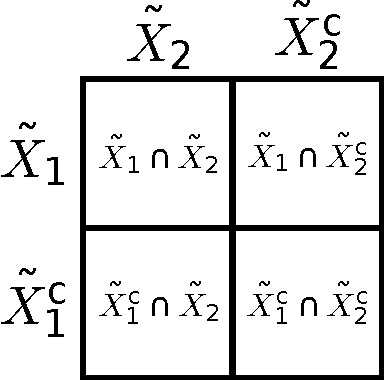
\includegraphics[width=0.5\linewidth]{figures/atoms-n2.pdf}
    \caption{Exemplo de átomos para $n=2$.}
    \label{fig:atoms-n2}
  \end{marginfigure}
\end{example}

\begin{example}
  Considerando agora o caso com $n=3$.
  Teremos os conjuntos $\tilde{X}_1, \tilde{X}_2, \tilde{X}_3$ e seus complementos,
  respectivamente, $\tilde{X}_1^c, \tilde{X}_2^c, \tilde{X}_3^c$. Existirão $8$ átomos:
  $\tilde{X}_1 \cap \tilde{X}_2 \cap \tilde{X}_3$,
  $\tilde{X}_1 \cap \tilde{X}_2 \cap \tilde{X}_3^c$,
  $\tilde{X}_1 \cap \tilde{X}_2^c \cap \tilde{X}_3$,
  $\tilde{X}_1 \cap \tilde{X}_2^c \cap \tilde{X}_3^c$,
  $\tilde{X}_1^c \cap \tilde{X}_2 \cap \tilde{X}_3$,
  $\tilde{X}_1^c \cap \tilde{X}_2 \cap \tilde{X}_3^c$,
  $\tilde{X}_1^c \cap \tilde{X}_2^c \cap \tilde{X}_3$, e
  $\tilde{X}_1^c \cap \tilde{X}_2^c \cap \tilde{X}_3^c$,
  como representados na \Cref{fig:atoms-n3}.
  \begin{marginfigure}%
    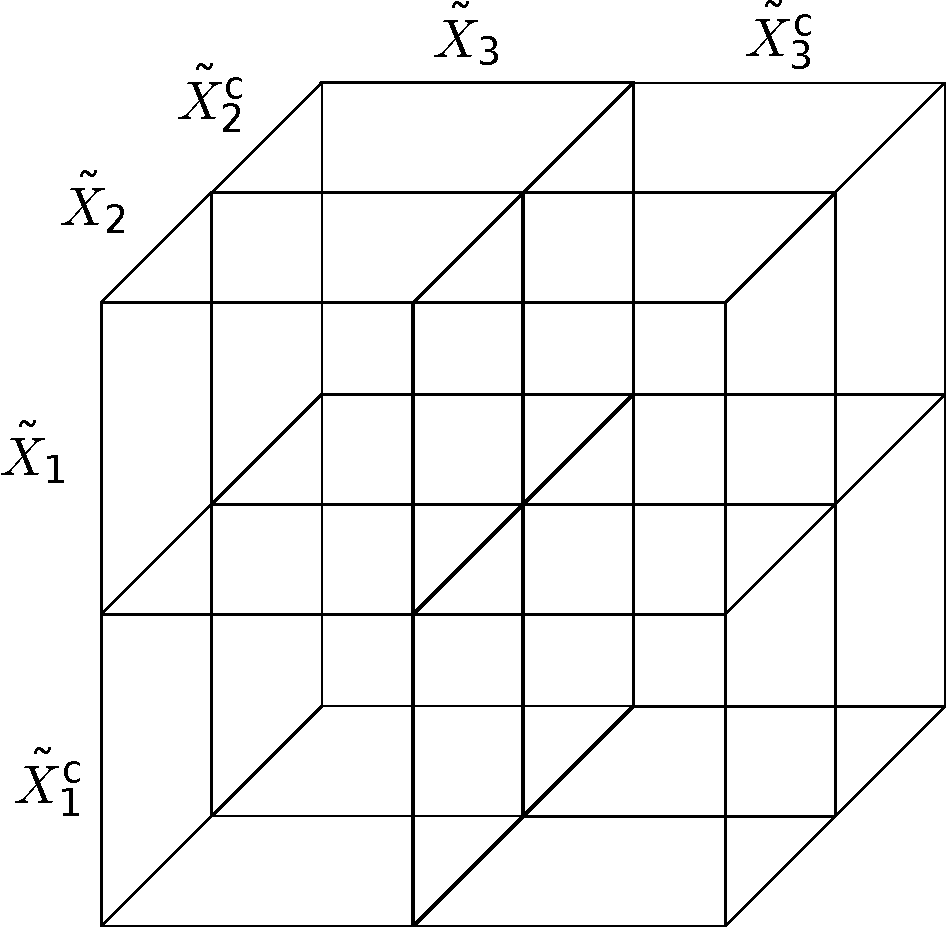
\includegraphics[width=0.75\linewidth]{figures/atoms-n3.pdf}
    \caption{Exemplo de átomos para $n=3$.}
    \label{fig:atoms-n3}
  \end{marginfigure}
\end{example}

Consideremos $n$ variáveis aleatórias discretas $X_1, X_2, \ldots, X_n$,
onde cada $X_i$ tem um suporte finito $S_{X_i}$, com $\vert S_{X_i} \vert = k_i$,
e os suportes $S_{X_i}$ podem ser distintos.
Por exemplo, $S_{X_1} = \{0,1\}$, $S_{X_2} = \{a,b,c\}$, e assim por diante. 
O espaço amostral é o produto cartesiano $\Omega = S_{X_1} \times S_{X_2} \times \ldots \times S_{X_n}$,
com $\vert \Omega \vert = k_1 \cdot k_2 \cdot \ldots \cdot k_n$, e o campo $F_n = 2^{\Omega}$
contém todos os subconjuntos de $\Omega$. Nesse contexto, os átomos são os eventos
$\{(X_1, \ldots, X_n) = (x_1, \ldots, x_n)\}$, e grandezas como a entropia $H(X_1,\ldots,X_n)$
podem ser interpretadas como medidas sobre $F_n$.
Para ilustrar propriedades específicas, consideremos o caso particular em que $S_{X_i} = \{0,1\}, \forall i$,
ou seja, $\Omega = \{0,1\}^n$, com $\vert \Omega \vert = 2^n$ e $F_n = 2^\Omega$.
Nesse cenário, teremos as seguintes propriedades:
\begin{enumerate}
  \item há exatamente $2^n$ átomos;
  \item $\vert F_n \vert = 2^\Omega = 2^{2^n}$;
  \item Todos os átomos em $F_n$ são disjuntos;
  \item Todo conjunto $A \in F_n$ pode ser expresso de forma única como uma união de um subconjunto dos átomos.
\end{enumerate}

Em análise matemática, uma medida em um conjunto $S$ é uma forma sistemática de atribuir
números a todo subconjunto de $S$, sendo intuitivamente interpretada como o seu tamanho.
Medida com sinal é uma generalização do conceito de medida permitindo que esta assuma valores
negativos.

\begin{definition}[Medida com sinal]
  Uma função real $\mu$ definida em $\mathcal{F}_n$ é chamada medida com sinal se
  for aditiva no conjunto, i.e., para $A$ e $B$ disjuntos em $\mathcal{F}_n$,
  \begin{equation}
  \mu(A \cup B) = \mu(A) + \mu(B) .
  \end{equation}
\end{definition}
Para uma medida com sinal $\mu$ teremos $\mu(\emptyset)=0$, já que
$\mu(A) = \mu(A \cup \emptyset) = \mu(A) + \mu(\emptyset)$.

Uma medida com sinal $\mu$ em $\mathcal{F}_n$ é completamente especificada
por seus valores nos átomos de $\mathcal{F}_n$. Os valores de $\mu$ em outros
conjuntos de $\mathcal{F}_n$ podem ser obtidos pela aditividade de conjuntos,
já que qualquer $\tilde{X} \in \mathcal{F}_n$ pode ser representado como
$\tilde{X} = \cup_{i=1} Y_i$, onde $Y_i$ são átomos escolhidos apropriadamente.

\begin{example}[$n=2$]
  Uma medida com sinal $\mu$ em $\mathcal{F}_2$ é completamente especificada pelos
  valores
  $\mu( \tilde{X}_1 \cap \tilde{X}_2 )$,
  $\mu( \tilde{X}_1 \cap \tilde{X}_2^c )$,
  $\mu( \tilde{X}_1^c \cap \tilde{X}_2 )$, e
  $\mu( \tilde{X}_1^c \cap \tilde{X}_2^c )$.

  O valor de $\mu$ em $\tilde{X}_1$ pode ser obtido da seguinte forma
  \begin{subequations}
    \begin{align}
      \mu( \tilde{X}_1 ) &= \mu( (\tilde{X}_1 \cap \tilde{X}_2) \cup ( \tilde{X}_1 \cap \tilde{X}_2^c) ) \\
                &= \mu( \tilde{X}_1 \cap \tilde{X}_2 ) + \mu( \tilde{X}_1 \cap \tilde{X}_2^c ) .
    \end{align}
  \end{subequations}

  O valor de $\mu$ em $\tilde{X}_1 \setminus \tilde{X}_2$ é dado por
  \begin{equation}
  \mu( \tilde{X}_1 \setminus \tilde{X}_2 ) = \mu( \tilde{X}_1 \cap \tilde{X}_2^c ) .
  \end{equation}

  O valor de $\mu$ em $\tilde{X}_1 \cup \tilde{X}_2$ pode ser obtido através de
  \begin{subequations}
    \begin{align}
      \mu( \tilde{X}_1 \cup \tilde{X}_2 ) &=& \mu( (\tilde{X}_1 \cap \tilde{X}_2) \cup (\tilde{X}_1 \cap \tilde{X}_2^c) \cup (\tilde{X}_1^c \cap \tilde{X}_2) ) \\
        &=& \mu( \tilde{X}_1 \cap \tilde{X}_2 ) + \mu( \tilde{X}_1 \cap \tilde{X}_2^c ) + \mu(\tilde{X}_1^c \cap \tilde{X}_2)
    \end{align}
  \end{subequations}

\end{example}

Os conjuntos $\tilde{X}_1$ e $\tilde{X}_2$ estão associados às variáveis
aleatória $X_1$ e $X_2$. O campo $\mathcal{F}_2$ é gerado por $\tilde{X}_1$ e $\tilde{X}_2$,
através dos átomos
$(\tilde{X}_1 \cap \tilde{X}_2)$,
$(\tilde{X}_1 \cap \tilde{X}_2^c)$,
$(\tilde{X}_1^c \cap \tilde{X}_2)$, e
$(\tilde{X}_1^c \cap \tilde{X}_2^c)$.
O diagrama de informação é apresentado na Figura \ref{fig:setX1X2}.
  \begin{marginfigure}%
    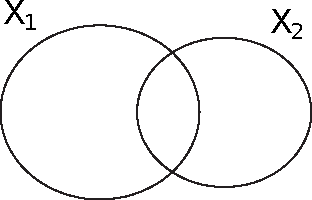
\includegraphics[width=0.5\linewidth]{figures/setX1X2.pdf}
    \caption{Diagrama de informação para $X_1$ e $X_2$.}
    \label{fig:setX1X2}
  \end{marginfigure}

O conjunto universo será considerada como sendo $\Omega = \tilde{X}_1 \cup \tilde{X}_2$.
  Desta forma, o átomo $\tilde{X}_1^c \cap \tilde{X}_2^c$ se degenera ao conjunto vazio,
  \begin{equation}
  \tilde{X}_1^c \cap \tilde{X}_2^c = (\tilde{X}_1 \cup \tilde{X}_2)^c = \Omega^c = \emptyset .
  \end{equation}

  Para as v.a.s $X_1$ e $X_2$, as medidas de informação de Shannon são
  \begin{equation}
  H(X_1), H(X_2), H(X_1|X_2), H(X_2|X_1), H(X_1,X_2), I(X_1;X_2) .
  \end{equation}

  Utilizando a notação $A \cap B^c \equiv A \setminus B$, definimos uma medida com sinal $\mu^\ast$
  \begin{subequations}
  \begin{align}
  \mu^\ast(\tilde{X}_1 \setminus \tilde{X}_2) &= H(X_1|X_2) ,\\
  \mu^\ast(\tilde{X}_2 \setminus \tilde{X}_1) &= H(X_2|X_1) ,\\
  \mu^\ast(\tilde{X}_1 \cap \tilde{X}_2) &= I(X_1;X_2) .
  \end{align}
  \end{subequations}
  Estes são os valores de $\mu^\ast$ nos átomos não vazios de $\mathcal{F}_2$.
  Os valores de $\mu^\ast$ nos demais conjuntos de $\mathcal{F}_2$ podem ser obtidos por
  adição de conjuntos. Em particular, temos as relações
  \begin{subequations}
  \begin{align}
  \mu^\ast(\tilde{X}_1 \cup \tilde{X}_2) &= H(X_1, X_2) , \label{eqX1X2HX1X2} \\
  \mu^\ast(\tilde{X}_1) &= H(X_1) , \label{eqmuX1HX1}\\
  \mu^\ast(\tilde{X}_2) &= H(X_2) .
  \end{align}
  \end{subequations}

Por exemplo, a Equação \ref{eqX1X2HX1X2} pode ser verificada
\begin{subequations}
  \begin{align}
  \mu^\ast(\tilde{X}_1 \cup \tilde{X}_2) &= \mu^\ast( (\tilde{X}_1 \setminus \tilde{X}_2) \cup (\tilde{X}_2 \setminus \tilde{X}_1) \cup (\tilde{X}_1 \cap \tilde{X}_2) ) \nonumber \\
        &= \mu^\ast( \tilde{X}_1 \setminus \tilde{X}_2 ) + \mu^\ast( \tilde{X}_2 \setminus \tilde{X}_1 ) + \mu^\ast( \tilde{X}_1 \cap \tilde{X}_2 ) \nonumber \\
        &= H(X_1|X_2) + H(X_2|X_1) + I(X_1;X_2) \nonumber \\
        &= H(X_1, X_2) .
  \end{align}
\end{subequations}


A Equação \ref{eqmuX1HX1} também pode ser facilmente verificada
\begin{subequations}
  \begin{align}
  \mu^\ast(\tilde{X}_1) &= \mu^\ast( (\tilde{X}_1 \cap \tilde{X}_2) \cup (\tilde{X}_1 \cap \tilde{X}_2^c) ) \nonumber \\
        &= \mu^\ast(\tilde{X}_1 \cap \tilde{X}_2) + \mu^\ast(\tilde{X}_1 \cap \tilde{X}_2^c) \nonumber \\
        &= I(X_1;X_2) + H(X_1|X_2) = H(X_1) .
  \end{align}
\end{subequations}

  É possível então verificar a seguinte correspondência com as medidas de informação de Shannon
  \begin{subequations}
  \begin{align}
  H / I &\leftrightarrow \mu^\ast \\
  , &\leftrightarrow \cup \\
  ; &\leftrightarrow \cap \\
  | &\leftrightarrow \setminus
  \end{align}
  \end{subequations}

Com a notação de medida, não existe distinção entre $H$ e $I$, podemos escrever
$H(X;Y) = I(X;Y)$, utilizando a notação do ponto-e-vírgula.





\chapter{Propriedade da Equipartição Assintótica}

A Propriedade da Equipartição Assintótica (AEP) visa analisar o comportamento
de sequências no limite, quando estas sequências tornam-se muito grandes.  A
AEP mostra que para uma sequência longa de variáveis aleatórias independentes e
identicamente distribuídas (i.i.d.), a probabilidade de observar uma sequência
típica é aproximadamente $2^{-nH(X)}$, onde $H(X)$ é a entropia da fonte e $n$
o comprimento da sequência.

Primeiramente, vamos rever o conceito de estatística de uma amostra.
\begin{definition}[Estatístima amostral]
    Seja $x_1, x_2, \ldots, x_n$ uma sequência de comprimento $n$ de valores observados
    de uma amostra de tamanho $n$, obtidos a partir da realização de variáveis aleatórias
    $X_1, X_2, \ldots, X_n$, uma estatística de uma amostra é qualquer função calculada a partir
    de uma amostra de dados, $T(x_1, x_2, \ldots, x_n)$.
\end{definition}
Exemplos comuns incluem a média amostral
\begin{equation}
  \bar{x} = T(x_1, \ldots, x_n) = \frac{1}{n} \sum_{i=1}^n x_i ,
\end{equation}
a variância amostral
\begin{equation}
  s^2 = T(x_1, \ldots, x_n) = \frac{1}{n-1} \sum_{i=1}^n (x_i - \bar{x})^2 ,
\end{equation}
a mediana amostral, a primeira amostra $x_1$, a última amostra $x_n$,
ou até estatísticas como o máximo ou mínimo da amostra, que capturam aspectos específicos dos dados observados.
Quando avaliamos $T$ nas variáveis aleatórias $X_1, X_2, \ldots, X_n$, o resultado $T(X_1,X_2,\ldots,X_n)$
é uma variável aleatória, com sua própria distribuição.


\begin{example}[Ensaio de Bernoulli]\label{ex:ensaiobernoulliT}
  Considere o experimento de Bernoulli com $X_1, \ldots, X_n$ i.i.d., com $X_i \in \{0, 1\}$ e
  parâmetro $\theta = Pr(X_i == 1)$.

  Uma dada sequência qualquer $x_1, \ldots, x_n$ terá então probabilidade dada por
  \begin{equation}
  p(x_1,x_2,\ldots,x_n) = \prod_{i=1}^n \theta^{x_i} (1-\theta)^{1-x_i} = \theta^{\sum_i x_i} (1-\theta)^{n - \sum_i x_i}
  \end{equation}

  Considere agora a seguinte estatística
  \begin{equation}
    T(x_1,\ldots, x_n) = \sum_{i=1}^{x} x_i ,
  \end{equation}
  o somatório da amostra, no caso, a quantidade de valoes iguais a 1 que apareceu em uma realização.
  Uma vez que sabemos tal estatísticas, a probabilidade de uma sequência pode ser expressa
  sem fazer referência à $\theta$ (parâmetro que caracteriza a distribuição).
  \begin{subequations}\label{eq:TsuficienteSum}
    \begin{align}
      p(x_1,\ldots,x_n|T(x_1,\ldots,x_n),\theta) &= p(x_1,\ldots,x_n|T(x_1,\ldots,x_n)) \\
                                                &= \begin{cases}
                                                   \frac{1}{{n \choose k}} & , \sum_i x_i = k \\
                                                   0       & , \text{caso contrário}.
                                                   \end{cases}
    \end{align}
  \end{subequations}
  Em outras palavras, $X_{1:N} \independent \theta | T(X_{1:N})$. 
  Isto implica na cadeia de Markov $\theta \rightarrow T(X_{1:N}) \rightarrow X_{1:N}$.
  Aplicando a desigualdade de processamento de dados, obtemos
  \begin{equation}\label{eq:dpdtberex01}
    I(\theta;T(X_{1:N})) \geq I(\theta;X_{1:N}).
  \end{equation}
  Por outro lado, sabemos que $T(X_{1:N})$ é uma função de $X_{1:N}$.
  Desta forma, também temos a seguinte cadeia de Markov: $\theta \rightarrow X_{1:N} \rightarrow T(X_{1:N})$.
  Novamente, aplicando a desigualdade de processamento de dados, obtemos
  \begin{equation}\label{eq:dpdtberex02}
    I(\theta;X_{1:N}) \geq I(\theta;T(X_{1:N})).
  \end{equation}
  Então, para que \ref{eq:dpdtberex01} e \ref{eq:dpdtberex02} sejam satisfeitos, devemos ter
  \begin{equation}
    I(\theta;X_{1:N}) = I(\theta;T(X_{1:N})) ,
  \end{equation}
  e nenhuma informação é perdida sobre $\theta$ indo de $X_{1:N}$ para $T(X_{1:N})$.
\end{example}





\begin{definition}[Estatística Suficiente]
Uma função $T(\cdot)$ é dita ser uma estatística suficiente em relação à família
$\{f_{\theta} (x)\}$ se $X$ é independente de $\theta$ dado $T(X)$ para qualquer
distribuição em $\theta$ (i.e. $\theta \rightarrow T(X) \rightarrow X$ forma uma
cadeia de Markov). Então
\begin{equation}
I(\theta ; X) = I(\theta ; T(X)), \; \forall \theta
\end{equation}
Uma estatística suficiente preserva a informação mútua e reciprocamente
\begin{equation}
X \independent \theta | T(X) .
\end{equation}
\end{definition}

Podemos verificar que, no \Cref{ex:ensaiobernoulliT}, a estatísticas utilizada
é uma estatísticas suficiente (veja a \Cref{eq:TsuficienteSum}).


Um critério prático para identificar estatísticas suficientes é dado pelo Teorema da Fatoração de Fisher-Neyman.
\begin{theorem}
Uma estatísticas $T(X_1,\ldots,X_N)$ é suficiente para $\theta$ se, e somente se,
a função de verossimilhança da amostra pode ser escrita como:
\begin{equation}
  \mathcal{L}(\theta;x_1,\ldots,x_n) = g(T(x_1,\ldots,x_n),\theta) \cdot h(x_1,\ldots,x_n) ,
\end{equation}
onde $g$ é uma função que depende de $\theta$ e da estatística $T$, e $h$ é uma função que não depende de $\theta$.
\end{theorem}
A demonstração e mais informações sobre o tema podem ser vistos em \textcite{berger2002}.





O histograma empírico da amostra é uma estatística que descreve a distribuição de frequências relativas dos valores observados em uma amostra. 
\begin{definition}[Histograma Empírico]
  Para uma amostra $x_1,x_2,\ldots,x_n$, obtida a partir de variáveis aleatórias $X_1,X_2,\ldots,X_n$,
  com suporte finito $S_X = \{a_1,a_2,\ldots,a_D\}$, o histograma empírico pode ser definido como a
  função que associa cada símbolo $a \in S_X$ à sua frequência relativa:
  \begin{equation}
  \hat{p}_n(a) = \frac{1}{n} \sum_{i=1}^n I\{ x_i = a \} ,
  \end{equation}
  onde $I\{ x_i = a \}$ é a função indicadora
  \begin{equation}
    I\{ x_i = a \} = \begin{cases}
      1, & x = a,\\
      0, & x\neq a. 
    \end{cases}
  \end{equation}
  Desta forma, $\hat{p}_n(a)$ representa a proporção de vezes que o valor $a$ aparece na amostra.
\end{definition}
Equivalentemente, o histograma empírico pode ser representado como a enúpla que contém as frequências relativas de todos os símbolos de $S_X$.
\begin{equation}
P_{x_{1:n}} \triangleq \left( \frac{N(a_1|x_{1:n})}{n} , \frac{N(a_2|x_{1:n})}{n} , \ldots , \frac{N(a_D|x_{1:n})}{n} \right) ,
\end{equation}
onde $N(a_i|x_{1:n})$ é a contagem do número de ocorrências do símbolo $a_i$ na amostra $x_{1:n}$.
O histograma é uma estatística, já que é uma função da amostra. Podemos mostrar ainda que
o histograma empírico é uma estatísticas suficiente:
\begin{subequations}
  \begin{align}
    p(x_{1:n}|P_{x_{1:n}},\theta) &=
                \begin{cases}
                \frac{1}{{n \choose {n_1, n_2, \ldots, n_D}}} & , n_i = n P_{x_{1:n}}(a_i), \forall i \\
                0       & , \text{caso contrário}
                \end{cases} \\
                &= p(x_{1:n} \vert P_{x_{1:n}})
  \end{align}
\end{subequations}
onde temos o coeficiente multinomial\footnote{
  Teorema Multinomial
        \begin{equation}
        (x_1 + x_2 + \ldots + x_m)^n = \sum_{k_1 + k_2 + \ldots + k_m = n} {n \choose {k_1, k_2, \ldots, k_m}} \prod_{1 \leq t \leq m} x_t^{k_t}
        \end{equation}
}
${n \choose {k_1, k_2, \ldots, k_m}} = \frac{n!}{k_1! k_2! \ldots k_m!}$.
Podemos observar que $p(x_{1:n}|P_{x_{1:n}},\theta) = p(x_{1:n}|P_{x_{1:n}})$, ou seja,
é independente de $\theta$.
Então $X_{1:n} \independent \theta \vert P_{x_{1:n}}$, então $P_{x_{1:n}}$ é uma estatística suficiente.






\section{Codificação}

O codificador é responsável por associar cada sequência $x_1,x_2,\ldots,x_n$
produzida pela fonte, ou seja, realizações de variáveis aleatórias $X_1,X_2,\ldots,X_n$,
a uma sequência de bits de comprimento variável ou fixo, de modo que a sequência original 
possa ser recuperada perfeitamente por um decodificador. Para simplificar, vamos
supor que as mensagens codificadas possuem, todas elas, um mesmo comprimento $m$.
O alfabeto da fonte é $\mathcal{X} = \{a_1, a_2, \ldots, a_K\}$, possuindo assim 
cardinalidade $K = \vert \mathcal{X} \vert$. O alfabeto
de saída do codificador é $\mathcal{Y} = \{0,1\}$, ou seja, codificação binária ($\vert \mathcal{Y} \vert = 2$).
A \Cref{fig:blockcoding} representa este esquema de codificação.

\begin{figure}%
  \centering
  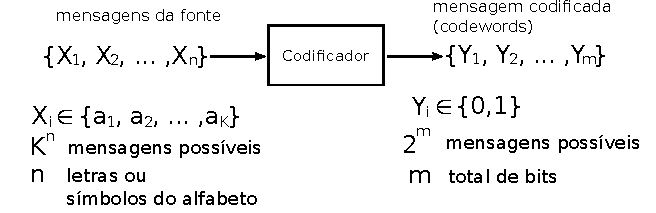
\includegraphics[width=0.8\linewidth]{figures/blockcoding.pdf}
  \caption{Esquemático de um codificador.}
  \label{fig:blockcoding}
\end{figure}

Para que seja possível termos uma palavra de código para cada mensagem possível,
devemos satisfazer a seguinte condição:
\begin{equation}
  2^m \geq K^n ,
\end{equation}
ou seja,
\begin{equation}
  m \geq (\log K) n
\end{equation}

A taxa de codificação mede a eficiência de um esquema de codificação 
ao representar uma sequência de símbolos em forma binária. 
\begin{definition}[Taxa de Codificação]
  Para uma sequência de entrada de comprimento $n$, $X_1,X_2,\ldots,X_n$,
  codificada em uma mensagem binária de comprimento $m$, $Y_1,Y_2,\ldots,Y_m$,
  a taxa de codificação é definida como
  \begin{equation}
    R = \frac{m}{n} .
  \end{equation}
  $R$ representa então o número de bits por símbolo utilizados na tarefa de codificação.
\end{definition}



Considerando que a fonte produz uma sequência de símbolos i.i.d., a probabilidade de uma
sequência qualquer de comprimento $n$ pode ser expressa por
\begin{equation}
p(X_1 = x_1, X_2 = x_2, \ldots, X_n = x_n) = \prod_{i=1}^{n} p(X_i = x_i)
\end{equation}
A informação sobre um evento é dada por $-\log p(x) = I(x)$, então a informação
associada à mensagem $x_1,x_2,\ldots,x_n$ é 
\begin{subequations}
  \begin{align}
    I(x_1,x_2,\ldots,x_n) &= - \log p(x_1, x_2, \ldots, x_n) = - \log \prod_{i=1}^n p(x_i) \\
                          &= \sum_{i=1}^n - \log p(x_i) = \sum_{i=1}^n I(x_i),
  \end{align}
\end{subequations}
onde notamos que eventos independentes são aditivos em relação a esta função de informação.
Observe que $E I(X) = H(X)$.
A lei fraca dos grandes números\footnote{
Lei dos Grandes Números: 
Se um evento de probabilidade $p$ é observado repetidamente em ocasiões independentes,
a proporção da frequência observada deste evento em relação ao total número de repetições
converge em direção a $p$ à medida que o número de repetições se torna arbitrariamente grande.

Sejam $X_1, X_2, \ldots, X_n$ v.a.s i.i.d. com $\E X_i = \mu$ e $\Var X_i = \sigma^2 < \infty$, para $i=1,\ldots,n$.
Seja a média definida por $\overline{X_n} = \frac{1}{n} \sum_{i=1}^{n} X_i$, então, para $\varepsilon > 0$,
a \emph{Lei Fraca dos Grandes Números} diz que $\overline{X_n}$ converge em probabilidade para $\mu$, ou seja,
\begin{equation}
\lim_{n \rightarrow \infty} P \left( \vert \overline{X_n} - \mu \vert < \varepsilon  \right) = 1 .
\end{equation}
}
diz que $\frac{1}{n} S_n \xrightarrow{p} \mu$, onde $S_n$ é a soma
de v.a.s i.i.d. com média $\mu = \E X_i$. Temos que $I(X_i)$ também é uma v.a. com média $H(X)$.
Obteremos assim
\begin{equation}
  \frac{1}{n} \sum_{i=1}^n I(X_i) \xrightarrow[n \rightarrow \infty]{p} H(X) .
\end{equation}
Quando $n$ é grande suficiente, podemos escrever
\begin{subequations}
  \begin{align}
     \frac{1}{n} \sum_{i=1}^n I(x_i)        &\approx H(X) , \forall i, x_i \sim p(x) \\
     - \frac{1}{n} \sum_{i=1}^n \log p(x_i) &\approx H(X) \\
     - \log \prod_{i=1}^n p(x_i)            &\approx n H(X) \\
     - \log p(x_1,x_2,\ldots,x_n)           &\approx n H(X) \\
     p(x_1,x_2,\ldots,x_n)                  &\approx 2^{-nH(X)} .
  \end{align}
\end{subequations}
Esta probabilidade não depende da sequência em si. Depende apenas do comprimento $n$ e
da entropia da fonte.
Quando $n$ fica grande, podemos dizer que todas as sequências terão a mesma probabilidade: $2^{-nH}$.
Estas sequências que possuem esta probabilidade (praticamente todas as sequências) são
chamadas de \emph{sequências típicas}, e são representadas pela conjunto $A_\epsilon^{(n)}$.

Se todas as sequência de comprimento $n$ possuem aproximadamente a mesma probabilidade $2^{-nH(X)}$,
então existe no máximo $2^{nH}$ sequências de comprimento $n$. Pode ser que $2^{nH} \ll K^n$,
ou seja, o conjunto das sequências típicas é muito menor do que o conjunto de todas as sequências
possíveis de comprimento $n$. Isto implica que, efetivamente, poderemos nos preocupar apenas
com a codificação do conjunto menor, o conjunto das sequências que efetivamente ocorrem, as sequências
típicas. Desta forma, para representar (ou codificar) as sequencias típicas, precisaremos de
$nH(X)$ bits. Teremos então
\begin{equation}
m = nH(X)
\end{equation}
no modelo do codificador. Então a taxa será $H(X)$.


\begin{theorem}[Propriedade da Equipartição Assintótica]\label{thm-prop-eqp-ass}
  Se $X_1, X_2, \ldots, X_n$ são i.i.d. e $X_i \sim p(x)$ para todo $i$, então
  \begin{equation}\label{eq-pX1X2Xn-H}
  -\frac{1}{n} \log p(X_1, X_2, \ldots, X_n) \xrightarrow{p} H(X)
  \end{equation}
\end{theorem}
\begin{proof}
  \begin{subequations}
  \begin{align}
  -\frac{1}{n} \log p(X_1, X_2, \ldots, X_n) &= - \frac{1}{n} \log \prod_{i=1}^n p(X_i) \\
                                             &= - \frac{1}{n} \sum_i \log p(X_i) \xrightarrow{p} \E \log p(X) \label{eq:dempealfgn}\\
                                             &= H(X)
  \end{align}
  \end{subequations}
  onde utilizamos a lei fraca dos números grandes em \ref{eq:dempealfgn}.
  \end{proof}


\begin{definition}[Conjunto Típico]
  Um conjunto típico $A_\epsilon^{(n)}$ em relação a $p(x)$ é o conjunto de sequências
  $(x_1,x_2,\ldots,x_n) \in \mathcal{X}^n$ com propriedade
  \begin{equation}
  2^{-n(H(X)+\epsilon)} \leq p(x_1, x_2, \ldots, x_n) \leq 2^{-n(H(X)-\epsilon)}
  \end{equation}
  De forma equivalente, podemos escrever
  \begin{equation}
  A_\epsilon^{(n)} = \left\{ (x_1, x_2, \ldots, x_n) : \vert - \frac{1}{n} \log p(x_1, \ldots, x_n) - H \vert < \epsilon \right\}
  \end{equation}
\end{definition}



\begin{theorem}[Propriedades do Conjunto Típico $A_\epsilon^{(n)}$]\label{thm:propconjtip}
\ \\ 
\begin{enumerate}
\item\label{prop1conjtip} Se $(x_1, x_2, \ldots, x_n) \in A_\epsilon^{(n)}$, então
      \begin{equation}
      H(X) - \epsilon \leq - \frac{1}{n} \log p(x_1, x_2, \ldots, x_n) \leq H(X) + \epsilon
      \end{equation}
\item\label{prop2conjtip} $p(A_\epsilon^{(n)}) = p\left( \left\{ x: x \in A_\epsilon^{(n)} \right\} \right) > 1 - \epsilon$ para $n$ grande suficiente, para todo $\epsilon > 0$.
\item\label{prop3conjtip} Limite superior: $\vert A_\epsilon^{(n)} \vert \leq 2^{n(H(X)+\epsilon)}$, onde $\vert A_\epsilon^{(n)} \vert$ é o número de elementos no conjunto $A_\epsilon^{(n)}$.
\item\label{prop4conjtip} Limite inferior: $\vert A_\epsilon^{(n)} \vert \geq (1-\epsilon) 2^{n(H(X) - \epsilon)}$ para $n$ grande suficiente.
\end{enumerate}
\end{theorem}

\begin{proof}
\ \\
\begin{enumerate}
  \item O primeiro apenas é uma reformulação da definição de AEP.
  \item Vamos utilizar a definição expandida de convergência em probabilidade,
          dada na equação \ref{eq-pX1X2Xn-H}.
          \begin{equation}
          p(A_\epsilon^{(n)}) = p\left( \vert - \frac{1}{n} \sum_i \log p(x_i) - H \vert < \epsilon \right) > 1 - \delta
          \end{equation}
          para $n$ grande suficiente.
          Podemos escolher qualquer $\delta$, escolhemos então $\delta = \epsilon$, resultando em
          \begin{equation}
          p(A_\epsilon^{(n)}) > 1 - \epsilon, \quad \text{ para } n \text{ grande suficiente } \forall \epsilon
          \end{equation}
  \item Limite superior de $A_\epsilon^{(n)}$
    \begin{subequations}
      \begin{align}
        1 &= \sum_x p(x) \geq \sum_{x \in A_\epsilon^{(n)}} p(x) \geq \sum_{x \in A_\epsilon^{(n)}} 2^{-n(H(X)+\epsilon)} \\
          &= \vert A_\epsilon^{(n)} \vert 2^{-n(H(X)+\epsilon)}
      \end{align}
    \end{subequations}
  Resultando em $\vert A_\epsilon^{(n)} \vert \leq 2^{n(H+\epsilon)}$.
  \item Limite inferior do tamanho de $A_\epsilon^{(n)}$. Para $n$ grande suficiente
    \begin{subequations}
        \begin{align}
        1 - \epsilon &< p(A_\epsilon^{(n)}) \leq \sum_{x \in A_\epsilon^{(n)}} 2^{-n(H(X)-\epsilon)} \\
                     &= 2^{-n(H(X)-\epsilon)} \vert A_\epsilon^{(n)} \vert
        \end{align}
    \end{subequations}
    resultando em $\vert A_\epsilon^{(n)} \vert \geq (1-\epsilon) 2^{n(H(X)-\epsilon)}$.
\end{enumerate}
\end{proof}

A AEP e o tamanho do conjunto típico têm implicações diretas na codificação de
sequências, como no exemplo de imagens digitais. Considere uma imagem full HD
de $1080 \times 720$ pixels, com 16 milhões de cores (24 bits por pixel, ou
seja, $2^{24}$ cores possíveis). O número total de pixels é $1080 \times
720 = 777.600$, e cada pixel é representado por 24 bits, totalizando 
$K = 1080 \times 720 \times 24 = 18.662.400 \approx 10^7$ bits por imagem. O
número total de imagens possíveis é $2^K = 2^{18.662.400} \approx 10^{5.617 \times 10^6}$, 
um valor extremamente grande, muito maior que o número de
átomos no universo observável ($\approx 10^{81}$). Pela AEP, se os pixels
fossem i.i.d. com entropia $H(X)$ (em bits por pixel), o número de imagens
típicas seria aproximadamente $2^{nH(X)}$, onde $n = 777.600$. Mesmo
que $H(X)$ fosse pequeno (por exemplo, 1 bit por pixel devido a
redundâncias), o número de imagens típicas seria $2^{777.600} \approx 10^{234.000}$, 
ainda muito maior que $10^{81}$. Isso ilustra que, embora
o número de imagens típicas seja uma fração minúscula do total, ele ainda é
astronomicamente grande, destacando a necessidade de codificação eficiente para
lidar com sequências típicas, que dominam a probabilidade.

Considere agora as chaves privadas de Bitcoin. Uma
chave privada de Bitcoin é um número de 256 bits, gerado aleatoriamente, o que
significa que o número total de chaves possíveis é $2^{256} \approx 1,1579 \times 10^{77}$. 
Esse valor é menor que o número de átomos no universo observável, mas ainda é astronomicamente grande. 
Pela AEP, se os bits da chave fossem gerados de forma i.i.d. com entropia $H(X)$
(em bits por bit), o número de chaves típicas seria aproximadamente $2^{nH(X)}$, 
onde $n = 256$. No caso ideal, em que os bits são uniformes
($H(X) = 1$ bit por bit), o número de chaves típicas é $2^{256 \cdot 1} = 2^{256}$,
ou seja, todas as chaves são típicas. No entanto, se houvesse algum
viés na geração das chaves, por exemplo, $H(X) = 0,9$ bits por bit, o
número de chaves típicas seria $2^{256 \cdot 0,9} = 2^{230,4} \approx 10^{69,3}$, 
ainda um número enorme, mas uma fração do total. Isso ilustra a
importância de maximizar a entropia na geração de chaves para garantir que o
espaço de chaves típicas seja o maior possível, minimizando a probabilidade de
colisões.

\begin{marginfigure}%
  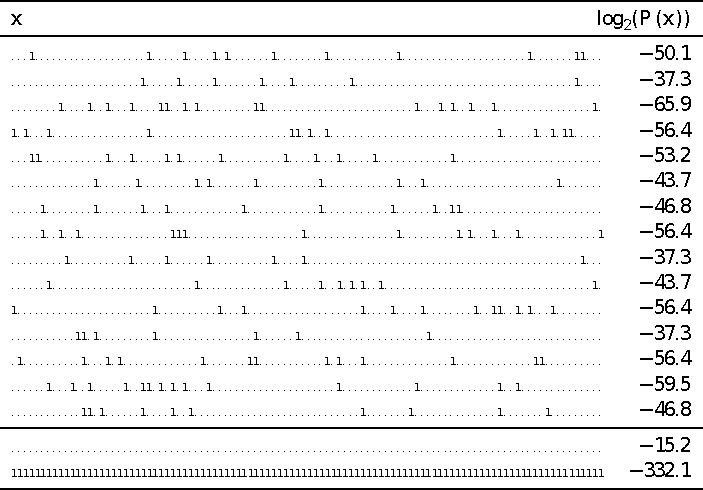
\includegraphics[width=\linewidth]{figures/seq100mackay.pdf}
  \caption{Sequências regadas por um ensaio de Bernoulli com $n=100$ e $P(X=1) = p = 0.1$.
        As 15 sequências superiores representam amostras típicas. As duas últimas sequências
        representam a sequência mais provável e a menos provável \parencite{mackay2003}.}
  \label{fig:seq100mackay}
\end{marginfigure}

Considere agora um ensaio de Bernoulli com $n = 100$ lançamentos, onde cada
lançamento $X_i$ é uma variável aleatória com $P(X_i = 1) = p = 0,1$ e
$P(X_i = 0) = 1-p = 0,9$. Nesse cenário, uma sequência 
$(x_1, x_2, \ldots, x_{100}) \in \{0,1\}^{100}$ tem probabilidade 
$P(x_1, \ldots, x_{100}) = p^k (1-p)^{n-k}$, onde $k = \sum_{i=1}^{100} x_i$ 
é o número de 1's na sequência. A \Cref{fig:seq100mackay} compara três tipos
de sequências: a mais provável, a menos provável e as sequências típicas.
A sequência mais provável é a sequência com 100 ocorrências de 0 (penúltima sequência
apresentada na \Cref{fig:seq100mackay}), já a sequência menos provável é aquela 
com 100 ocorrências de 1 (última sequência apresentada na \Cref{fig:seq100mackay}).
As sequências típicas são aquelas com probabilidade aproximadamente $2^{-nH(X)}$.
Para o exemplo em questão, temos $H = 0,4690$ e assim $\log (2^{-100 H(X)}) = -46.9$.
As 15 sequências apresentadas no parte superior da \Cref{fig:seq100mackay} representam
aquelas com $\log p(x_1,\ldots,x_n)$ próximo de $-46.9$, ou seja, sequências que
podemos considerar típicas (dado um determinado critério $\epsilon$).


\begin{figure}%
  \centering
  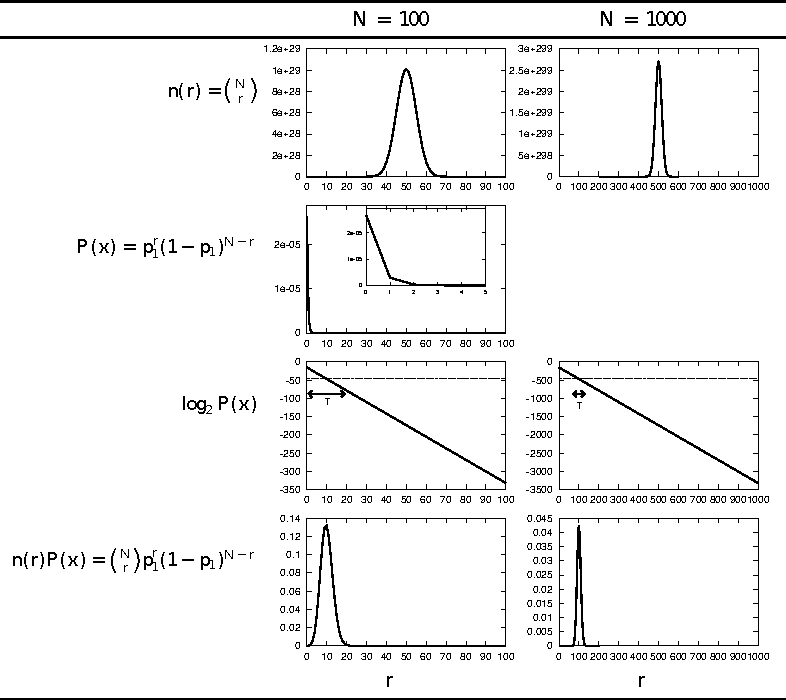
\includegraphics[width=\linewidth]{figures/seq100mackay2.pdf}
  \caption{Para $p=0.1$, $n=100$ e $n=1000$ os gráficos ilustram $n(r)$, o número de strings contendo 
    $r$ 1s; a probabilidade $P(x_{1:n})$ para uma string contendo $r$ 1s; a mesma probabilidade
    em escala logarítmica; e a probabilidade total $n(r) P(x_{1:n})$ de todas as strings contendo $r$ 1s \parencite{mackay2003}.
  }
  \label{fig:seq100mackay2}
\end{figure}

A \Cref{fig:seq100mackay2} ilustra o que ocorre quando $n$ cresce, fazendo assim
uma comparação para os casos $n=100$ e $n=1000$. Primeiramente, temos o número
de sequências de comprimento $n$ com $r$ ocorrências de 1's. Este número é dado
pelo coeficiente binomial. Nos extremos, existe apenas uma sequência com 100 zeros 
e uma sequência com 100 1's. No meio, teremos o pico, sequências com 50 ocorrências
de cada símbolo. Logo abaixo apresenta-se a probabilidade das sequências, que decai
rápidamente com o número de 1's presente na sequência. Por fim, temos o produto
dos dois gráficos anteriores, representando assim a probabilidade total das sequências
de um determinado tipo. Podemos observar, que o pico ocorre em sequências constituídas por
10\% de 1's. Verificamos ainda que este pico torna-se mais acentuado com o crescimento de $n$.
No limite, quando $n$ for muito grande, só ocorrerão sequências com 10\% de 1's.




\section{Codificação para o Conjunto Típico}

Após definirmos o que são sequências típicas e formalizarmos a propriedade da
equipartição assintótica, vamos agora abordar o problema de codificação
considerando a codificação de sequências típicas.  Como vimos que existe um
limite para o tamanho do conjunto típicos, iremos utilizar o número de bits
mínimo necessários para codificar as sequências quer pertençam a este conjunto.
As sequências remancessentes, contidas no conjunto não típico, podem ser
codificadas utilizando mais bits, sem que isto cause impacto significativo ao
código, uma vez que a probabilidade do conjunto típico é aproximadamente 1
(conforme \cref{prop2conjtip} do \Cref{thm:propconjtip}).

A ideia consiste em particionar o conjunto de sequencias em dois blocos:
conjunto típico $A_\epsilon^{(n)}$, e o seu complemento, o conjunto não típico 
$A_\epsilon^{(n)c} \triangleq \mathcal{X}^n \backslash A_\epsilon^{(n)}$.
Tais partições satisfazem $A_\epsilon^{(n)} \cap A_\epsilon^{(n)c} = \emptyset$, 
e $A_\epsilon^{(n)} \cup A_\epsilon^{(n)c} = \mathcal{X}^n$. A \Cref{fig:particao2}
ilustra o particionamento proposto.

\begin{marginfigure}%
  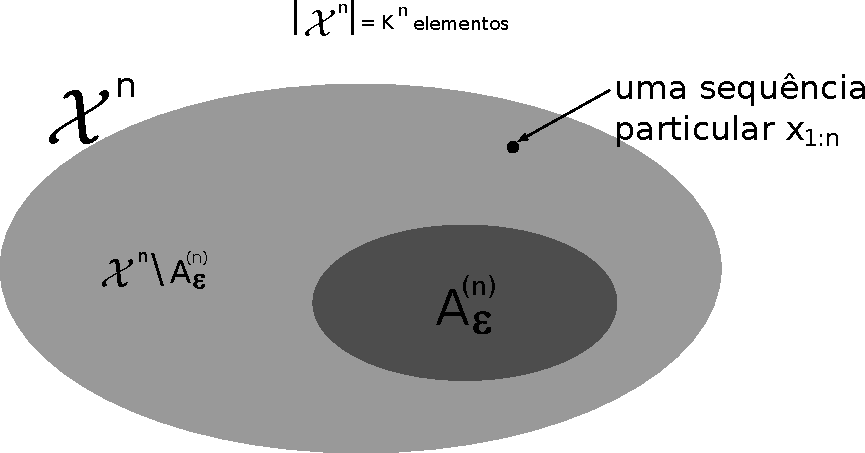
\includegraphics[width=\linewidth]{figures/particao2.pdf}
  \caption{Particionamento de $\mathcal{X}^n$ em dois conjuntos: $A_\epsilon^{(n)}$ e $A_\epsilon^{(n)c}$.}
  \label{fig:particao2}
\end{marginfigure}

Vamos então indexar os elementos de cada conjunto (conjunto típico e não-típico) separadamente.
O número de elementos do conjunto típico é $\vert A_\epsilon^{(n)} \vert \leq 2^{n(H+\epsilon)}$,
desta forma será necessário
\begin{equation}
  \lceil n(H+\epsilon) \rceil \leq n (H + \epsilon) + 1 \text{bits}
\end{equation}
para indexar os elementos deste conjunto.
Ainda, utilizaremos um bit extra para indicar se o elemento está no conjunto típico ou não, i.e.,
vamos utilizar uma sequência $(b_0,b_1,b_2,\ldots,b_{\lceil n(H+\epsilon) \rceil})$ onde
o primeiro bit indica se temos um elemento do conjunto típico ($b_0=0$) ou não
e os demais indexam o elemento do conjunto.
O número total de bits necessário para uma sequência típica será então $\leq n(H+\epsilon)+2$.

Para os elementos do conjunto não típico, vamos utilizar
\begin{equation}
  \lceil \log \vert \mathcal{X} \vert^n \rceil \leq n \log K + 1 \text{bits}.
\end{equation}
Então teremos um vetor binário da forma $(b_0,b_1,b_2,\ldots,b_{\lceil \log \vert \mathcal{X} \vert^n \rceil})$
onde $b_0=1$, indicando a atipicidade.
Assim, o número total de bits para indexar uma sequência atípica será $\leq n \log K + 2$.

Este código proposto é 1-pra-1, sendo fácil codificar e decodificar, dado o \textit{codebook}.
Para o conjunto não-típico $A_\epsilon^{(n)c}$ estamos utilizando mais bits do que o necessário,
já que $\vert A_\epsilon^{(n)c} \vert = \vert \mathcal{X}^n \vert - \vert A_\epsilon^{(n)} \vert = K^n - \vert A_\epsilon^{(n)} \vert \leq K^n$,
mas isto não importará, como veremos adiante.
O importante desta proposta de código é que as sequências típicas possuem um comprimento descritivo curto, aproximadamente $nH$.

\begin{definition}[Comprimento da palavra associada a uma sequência]
  O comprimento da palavra (\emph{codeword}) associada à sequência $x_{1:n}$ é denominado $l(x_{1:n})$.
\end{definition}
Assim, $l(X_{1:n})$ é uma variável aleatória, já que $X_{1:n}$ é uma variável aleatória.
Então $E l(X_{1:n}) = \sum_{x_{1:n}} p(x_{1:n}) l(x_{1:n})$ é o valor esperado do comprimento
do código. Queremos que ele seja o menor possível.

Suponha que $n$ seja grande suficiente de forma que $p(A_\epsilon^{(n)}) > 1 - \epsilon$, então
\begin{subequations}
  \begin{align}
    E l(X_{1:n}) &= \sum_{x_{1:n}} p(x_{1:n}) l(x_{1:n}) \\
                 &= \sum_{x_{1:n} \in A_\epsilon^{(n)}} p(x_{1:n}) l(x_{1:n}) + \sum_{x_{1:n} \in A_\epsilon^{(n)c}} p(x_{1:n}) l(x_{1:n}) \\
                 &\leq \sum_{x_{1:n} \in A_\epsilon^{(n)}} p(x_{1:n}) [n(H+\epsilon)+2] + \sum_{x_{1:n} \in A_\epsilon^{(n)c}} p(x_{1:n}) [n \log K + 2] \\
                 &= \underbrace{p(A_\epsilon^{(n)})}_{\leq 1} [n(H+\epsilon)+2] + \underbrace{p(A_\epsilon^{(n)c})}_{< \epsilon} [n \log K + 2] \\
                 &\leq n(H+\epsilon)+2 + \epsilon n \log K + \epsilon 2 \\
                 &= n [H + \underbrace{\epsilon + \epsilon \log K + \frac{2}{n} + \frac{2 \epsilon}{n}}_{\epsilon'} ] = n(H+\epsilon') ,
  \end{align}
\end{subequations}
onde definimos $\epsilon'$ como
\begin{equation}
  \epsilon' = \epsilon + \epsilon \log K + \frac{2}{n} + \frac{2 \epsilon}{n} .
\end{equation}
Podemos fazer $\epsilon'$ tão pequeno quanto queremos, fazendo $\epsilon$ pequeno e $n$ grande.
Desta forma, podemos fazer $n(H+\epsilon')$ tão próximo quanto quisermos de $nH$.

\begin{theorem}[Primeiro Teorema de Shannon]
Seja $X_{1:n}$ i.i.d. $\sim p(x)$, $\epsilon > 0$, então $\exists$ um código $f_n : \mathcal{X}^n \rightarrow \text{string binária}$
e um inteiro $n_{\epsilon}$, tal que o mapeamento seja um-pra-um (desta forma inversível sem erro), e
      \begin{equation}
      E[ \frac{1}{n} l(X_{1:n})] \leq H(X) + \epsilon
      \end{equation}
para todo $\epsilon > 0$ e todo $n \geq n_{\epsilon}$.
\end{theorem}

\begin{proof}
  A demonstração do Primeiro Teorema de Shannon usa a codificação de sequências típicas de maneira semelhante ao
  exemplo anterior.
\end{proof}


É interessante notar que a sequência mais provável não pertence ao conjunto
típico $A_\epsilon^{(n)}$. Isso ocorre porque o conjunto típico contém
sequências cujo histograma empírico é próximo da distribuição subjacente. A
tipicidade não está relacionada à probabilidade de uma única sequência ser a
maior. 

Dado que o conjunto típcio é tal que $P(A_\epsilon^{(n)}) \to 1$ à medida que
$n \to \infty$, ou seja, $A_\epsilon^{(n)}$ captura toda probabilidade, podemos
nos questionar se existe um conjunto ainda menor que também contenha
essencialmente `toda' a probabilidade.

\begin{definition}[Sequências asintoticamente iguais até a primeira ordem do expoente]\label{def:saiapoe}
A notação $a_n \circeq b_n$ indica que $a_n$ e $b_n$ são iguais até a primeira ordem do expoente,
ou seja, suas taxas de crescimento exponencial são as mesmas à medida que $n \to \infty$. 
Formalmente, isso significa que $\lim_{n \to \infty} \frac{1}{n} |\log a_n - \log b_n| = 0$, 
de modo que $\frac{1}{n} \log a_n \to \alpha$ e $\frac{1}{n} \log b_n \to \alpha$ 
para o mesmo $\alpha$. Para $n$ grande, $a_n$ e $b_n$ possuem aproximadamente o mesmo comportamento. 
\end{definition}

\begin{theorem}
Seja $X_{1:n}$ uma sequência i.i.d. $\sim p(x)$. Para $\delta < \sfrac{1}{2}$ e qualquer $\delta' > 0$,
se $P(B_{\delta}^{(n)}) > 1 - \delta$, então
\begin{equation}
\frac{1}{n} \log \vert B_{\delta}^{(n)} \vert >  H - \delta',
\end{equation}
se $n$ é grande suficiente. Teremos assim
\begin{equation}
\vert B_{\delta}^{(n)} \vert > 2^{n(H-\delta')} \approx 2^{nH}
\end{equation}

Usando a \Cref{def:saiapoe}, podemos então reescrever o teorema anterior da seguinte forma:

Se $\delta_n \rightarrow 0$ e $\epsilon_n \rightarrow 0$, então teremos
\begin{equation}
\vert B_{\delta_n}^{(n)} \vert \circeq \vert A_{\epsilon_n}^{(n)} \vert \circeq 2^{nH}.
\end{equation}
\end{theorem}
\begin{proof}
Seja $X_1, X_2, \ldots, X_n$ i.i.d. $\sim p(x)$. Seja $B_{\delta}^{(n)} \subset \mathcal{X}^n$ tal que
$\Pr(B_{\delta}^{(n)}) > 1 - \delta$. Fixe $\epsilon < \sfrac{1}{2}$.
Dados dois subconjuntos quaisquer $A$ e $B$ tais que $\Pr(A) > 1 - \epsilon_1$ e $\Pr(B) > 1 - \epsilon_2$.
Seja $A^c$ o complemento de $A$ e $B^c$ o complemento de $B$, então
\begin{equation}
P(A^c \cup B^c) \leq P(A^c) + P(B^c) .
\end{equation}

Como $P(A) > 1 - \epsilon_1$, teremos $P(A^c) \leq \epsilon_1$. De forma similar, $P(B^c) \leq \epsilon_2$.
Poderemos assim escrever
\begin{subequations}
\begin{align}
P(A \cap B) &= 1 - P(A^c \cup B^c) \\
        &\geq 1 - P(A^c) - P(B^c) \\
        &\geq 1 - \epsilon_1 - \epsilon_2.
\end{align}
\end{subequations}

Podemos reescrever a desigualdade anterior como
\begin{equation}
\Pr(A_{\epsilon}^{(n)} \cap B_{\delta}^{(n)}) \geq 1 - \epsilon - \delta .
\end{equation}

A probabilidade de um conjunto é dada pela soma das probabilidades de todos os elementos (sequências) neste conjunto, logo teremos
\begin{equation}
\Pr(A_{\epsilon}^{(n)} \cap B_{\delta}^{(n)}) = \sum_{x^n \in A_{\epsilon}^{(n)} \cap B_{\delta}^{(n)}} p(x^n)
\end{equation}
A probabilidade dos elementos no conjunto típico é limitada por $2^{-n(H-\epsilon)}$.

Desta forma teremos
\begin{subequations}
\begin{align}
 1 - \epsilon - \delta &\leq \Pr(A_{\epsilon}^{(n)} \cap B_{\delta}^{(n)}) \\
                &= \sum_{x^n \in A_{\epsilon}^{(n)} \cap B_{\delta}^{(n)}} p(x^n) \\
                &\leq \sum_{x^n \in A_{\epsilon}^{(n)} \cap B_{\delta}^{(n)}} 2^{-n(H-\epsilon)} \\
                &= \vert A_{\epsilon}^{(n)} \cap B_{\delta}^{(n)} \vert 2^{-n(H-\epsilon)} \\
                &\leq \vert B_{\delta}^{(n)} \vert 2^{-n(H-\epsilon)},
\end{align}
\end{subequations}
onde utilizamos $A_{\epsilon}^{(n)} \cap B_{\delta}^{(n)} \subseteq B_{\delta}^{(n)}$.

Poderemos reescrever então da seguinte forma,
\begin{equation}
\vert B_{\delta}^{(n)} \vert  >  2^{n(H-\epsilon)} ,
\end{equation}
onde $\epsilon > 0$.
\end{proof}











\section{Método de Típos}

O método de tipos refina a abordagem das sequências típicas, oferecendo uma
análise mais estruturada das propriedades assintóticas. O método de tipos
considera todas as possíveis distribuições empíricas (ou `tipos') que
sequências $x_{1:n}$ podem ter, agrupando-as em conjuntos de sequências que
compartilham um mesmo histograma empírico $\hat{p}_n(x_{1:n})$, ou
$P_{x_{1:n}}$. O conjunto de sequências de comprimento $n$ pode ser
particionado em subconjuntos de sequências de tipos distintos. Na AEP, o método
de tipos confirma que o número de sequências típicas é $\circeq 2^{nH(X)}$.
Vamos então estabelecer algumas definições.

\begin{definition}[Tipo]
  Seja $X_1, X_2, \ldots, X_n \equiv X_{1:n}$ uma amostra de comprimento $n$ de uma variável aleatória discreta $D$-ária.
  Então $x_i \in \mathcal{X}$ e o tamanho do alfabeto é $D=\vert \mathcal{X} \vert$, e $\mathcal{X}=\{a_1, a_2, \ldots, a_D\}$.
  Definimos a seguinte estatística, o histograma empírico da amostras, também chamado tipo da amostra:
  \begin{equation}
  P_{x_{1:n}} \triangleq \left( \frac{n(a_1|x_{1:n})}{n}, \frac{n(a_2|x_{1:n})}{n}, \ldots, \frac{n(a_D|x_{1:n})}{n} \right)
  \end{equation}
  onde $n(a_i|x_{1:n})$ representa o número de ocorrências do símbolo $a_i$ na amostra $x_{1:n}$.
\end{definition}
Note que $P_{x_{1:n}}$ pode ser considerado como uma função massa probabilidade.
Um tipo $\hat{p}$ é uma função de massa de probabilidade sobre $S_X$, 
definido como o histograma empírico $\hat{p}(a) = \frac{k_a}{n}$, 
onde $k_a = \sum_{i=1}^n \mathbb{I}\{x_i = a\}$ é o número de ocorrências do símbolo $a \in S_X$ na sequência, 
e $\sum_{a \in S_X} k_a = n$.

\begin{definition}[Conjunto de Tipos]
    O Conjunto de Tipos $\mathcal{P}_n$, ou $\mathcal{P}_n (\mathcal{X})$, para sequências de comprimento $n$ sobre um alfabeto finito $\mathcal{X}$ 
    é o conjunto de todas as possíveis distribuições empíricas (ou tipos) que podem ser formadas 
    por sequências $(x_1, x_2, \ldots, x_n) \in \mathcal{X}^n$.
\end{definition}
\begin{example}[Ensaio de Bernoulli]
Para sequências de comprimento $n$ geradas a partir de um ensaio de Bernoulli com alfabeto $\mathcal{X} = \{0,1\}$,
teremos o seguinte conjunto de tipos:
\begin{equation}\label{eq:exconjtiposbernoulli}
\mathcal{P}_n (\mathcal{X}) = \left\{ \left( \frac{0}{n}, \frac{n}{n} \right), \left( \frac{1}{n} , \frac{n-1}{n} \right), \ldots, \left( \frac{n}{n}, \frac{0}{n} \right)\right\}
\end{equation}
onde existem $n+1$ tipos (histogramas empíricos). O primeiro tipo em \ref{eq:exconjtiposbernoulli} representa
a sequência sem nenhuma ocorrência de zeros e $n$ ocorrências de uns; o segundo tipo representa 
as sequências com apenas uma ocorrência de zero e $n-1$ ocorrência de uns; e o último tipo
representa a sequência com $n$ ocorrência de zeros e nenhuma ocorrência de uns.
\end{example}


\begin{definition}[Classe de Tipo]
    A Classe de Tipo $T(P)$, ou $T(\hat{p})$, associada a um tipo $\hat{p} \in \mathcal{P}_n(\mathcal{X})$, 
    para sequências de comprimento $n$ sobre um alfabeto finito $\mathcal{X}$, 
    é o conjunto de todas as sequências $(x_1, x_2, \ldots, x_n) \in \mathcal{X}^n$ 
    que compartilham um mesmo histograma empírico $\hat{p}$, ou $P$.
    \begin{equation}
      T(P) \triangleq \{ x_{1:n} \in \mathcal{X}^n : P_{x_{1:n}} = P \} .
    \end{equation}
\end{definition}
\begin{example}[Ensaio de Bernoulli]
Para o caso do ensaio de Bernoulli, vejamos alguns exemplos de classe de tipo.

Para o tipo $P = \left( \frac{0}{n}, \frac{n}{n} \right)$, a classe de tipo $T(P)$ 
possui apenas uma sequência:
\begin{equation}
    T(P) = \{ 111\cdots{}11 \} .
\end{equation}

Para o tipo $P = \left( \frac{1}{n} , \frac{n-1}{n} \right)$, a classe de tipo $T(P)$
possui $n$ sequências:
\begin{equation}
    T(P) = \{ 011\cdots{}11, 101\cdots{}11, \ldots, 111\cdots{}01, 111\cdots{}10 \} .
\end{equation}

Para o tipo $P = \left( \frac{n}{n}, \frac{0}{n} \right)$, a classe de tipo $T(P)$
possui apenas uma sequência:
\begin{equation}
    T(P) = \{ 000\cdots{}00 \} .
\end{equation}
\end{example}


Como mencionado anteriormente, o conjunto de todas sequências $\mathcal{X}^n$
pode ser particionado em diferentes conjuntos $T(P_i)$, com $P_i \in \mathcal{P}_n$,
o conjunto de todos os tipos, ou seja, $\mathcal{P}_n = \{ P_1, P_2, \ldots, P_{\vert \mathcal{P}_n \vert} \}$.
As partições são disjuntas
\begin{equation}
    T(P_i) \cap T(P_j) = \emptyset, \forall i,j \in \{1, \ldots, \vert \mathcal{P}_n \vert\} \text{ e } i \neq j,
\end{equation}
e o particionamento é exaustivo
\begin{equation}
  \bigcup_{P \in \mathcal{P}_n} T(P) = \mathcal{X}^n.
\end{equation}
Este particionamento é ilustrado na \Cref{fig:particao-Xn2}.

\begin{marginfigure}%
  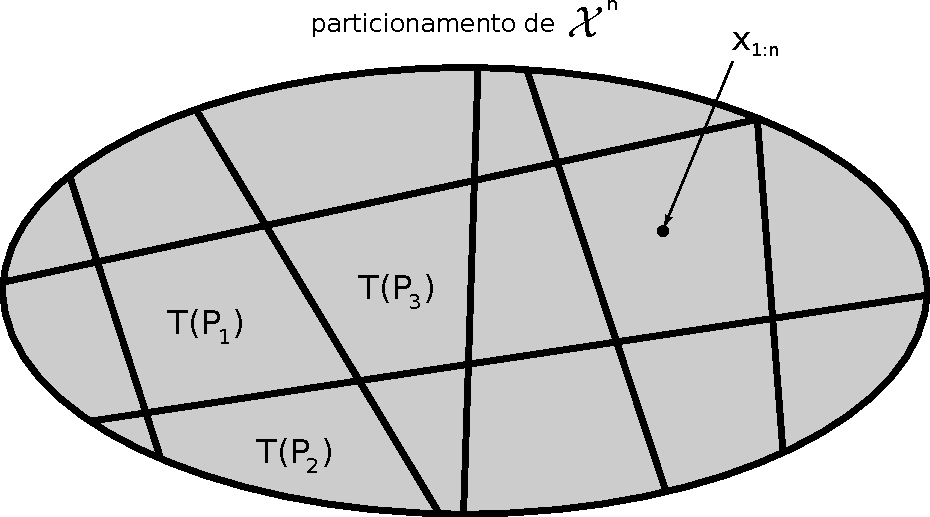
\includegraphics[width=\linewidth]{figures/particao-Xn2.pdf}
  \caption{Particionamento do espaço de sequências de comprimento $n$.}
  \label{fig:particao-Xn2}
\end{marginfigure}


No exemplo do ensaio de Bernoulli é fácil constatar quantos tipos distintos existem.
O \Cref{thm:numtiposn} a seguir usa o método estrela traço da análise combinatória para determinar
o número de tipos existentes. Vejamos então primeiramente o teorema da análise combinatória.

\begin{theorem}[Método Estrela Traço]
    Suponha que $n$ estrelas que devem ser organizadas em $k$ recipientes, podendo inclusive
    ter recipiente vazio.
    Neste caso, o número de maneiras de fazer tal organização é dado por
    \begin{equation}
	\binom{n+k-1}{k-1}
    \end{equation}
\end{theorem}
\begin{proof}
Este problema é o mesmo que incluir $k-1$ traços para separar uma sequência de $n$ estrelas.
Os traços podem ser inseridos em qualquer posição, inclusive sem existir estrelas entre eles,
como por exemplo, com $n=7$ e $k=4$:
$$\star \star \star \star \quad | \quad | \quad \star \quad | \quad \star \star$$
Note que, neste problema temos $n+k-1$ símbolos (estrelas e traços) para serem incluídos, dos
quais $k-1$ são escolhidos para serem traços. Desta forma existem $\tbinom{n+k-1}{k-1}$
formas de dispor estes símbolos.
\end{proof}

\begin{theorem}[Número de tipos existentes]\label{thm:numtiposn}
 Para sequências de comprimento $n$, em um alfabeto $\mathcal{X}$, o número de tipos é dado por
 \begin{equation}\label{eq:number-of-types}
 \vert \mathcal{P}_n \vert = {n + \vert \mathcal{X} \vert - 1 \choose \vert \mathcal{X} \vert - 1}
 \end{equation}
\end{theorem}
\begin{proof}
Um histograma empírico pode ser visto como uma variação do problema estrela-traço.
Se temos um alfabeto com $\vert\mathcal{X}\vert = D$ símbolos,
o Conjunto de Tipos $\mathcal{P}_n$ contém todas as possíveis distribuições empíricas $\hat{p}$
para sequências de comprimento $n$ sobre o alfabeto $\mathcal{X}$.
Um tipo $\hat{p}$ é uma função de massa de probabilidade tal que $\hat{p}(a) = \sfrac{k_a}{n}$,
onde $k_a$ é o número de ocorrências do símbolo $a \in \mathcal{X}$, e
$\sum_{a \in \mathcal{X}} k_a = n$. Assim, $k_a \in \{0,1, \ldots, n\}$, e a restrição
é que a soma de todos $k_a$'s deve ser igual a $n$, o comprimento da sequência.
Cada tipo $\hat{p}$ é definido pela ênupla $(k_{a_1}, k_{a_2}, \ldots, k_{a_D})$, e cada
uma delas corresponde a uma forma de organização no problema de estrelas e traços.
\end{proof}


Embora tenhamos uma fórmula fechada para o número de tipos, \Cref{eq:number-of-types},
iremos encontrar um limite superior para $\vert \mathcal{P}_n \vert$,
que, embora seja um limite relativamente largo, é mais fácil de manipular e suficiente 
para muitas demonstrações teóricas. 

\begin{theorem}[Limite no número de tipos]
 O número de tipos para sequências de comprimento $n$ em um alfabeto $\mathcal{X}$ é limitado por
 \begin{equation}\label{eq:number-of-types-bound}
 \vert \mathcal{P}_n \vert \leq (n+1)^{\vert \mathcal{X} \vert} .
 \end{equation}
\end{theorem}

\begin{proof}
 O numerador de cada entrada em um tipo pode assumir $(n+1)$ valores distintos (de $0$ a $n$).
 Existem $\vert \mathcal{X} \vert$ entradas em um tipo, e portanto a mesma quantidade de numeradores.
 Os valores dos numeradores interagem entre si (a soma de todos deve ser igual a $n$), mas podemos
 achar um limite superior desconsiderando esta interação.
 \begin{equation}
 \vert \mathcal{P}_n \vert \leq \underbrace{(n+1)\times(n+1)\times\ldots\times(n+1)}_{\vert \mathcal{X} \vert \text{ vezes}} = (n+1)^{\vert \mathcal{X} \vert} .
 \end{equation}
\end{proof}

É importante notar na \Cref{eq:number-of-types-bound} que existe no máximo um número polinomial em
$n$ de tipos de sequencias de comprimento $n$. Entretanto, sabemos que o número de sequências cresce com $n$,
$\vert \mathcal{X} \vert^n$. Com $n$ grande suficiente, eventualmente, teremos que apenas um único tipo
(o tipo das sequências típicas) conterá todas as sequências, como será demonstrado no \Cref{thm:teocodshannontipos}.


Para sequências geradas por uma fonte i.i.d., a probabilidade de uma sequência
$(x_1, x_2, \ldots, x_n)$ depende apenas do seu tipo e não da sequência específica.
Isso significa que todas as sequências em uma mesma classe de tipo, ou seja,
sequências que compartilham um mesmo histograma empírico, têm a mesma probabilidade.

\begin{theorem}[Probabilidade Depende do Tipo]
Seja $X_1, X_2, \ldots, X_n$ i.i.d. $\sim Q(x)$, com $Q$ arbitrário, e extensão
$Q^n(x_{1:n}) = \prod_i Q(x_i)$, a probabilidade da sequencia depende apenas do tipo, ou seja,
a probabilidade é `independente' da sequencia, dado o tipo e $Q$, isto é,
\begin{equation}
Q^n(x_{1:n}) = 2^{-n[ H(P_{x_{1:n}}) + D(P_{x_{1:n}}||Q) ]} .
\end{equation}
\end{theorem}

\begin{proof}
\begin{subequations}
\begin{align}
  Q^n(x_{1:n}) &= \prod_{i=1}^{n} Q(x_i) = \prod_{a \in \mathcal{X}} Q(a)^{n(a \mid x_{1:n})} \\
        &= \prod_{a \in \mathcal{X}} Q(a)^{n P_{x_{1:n}}(a) } = \prod_{a \in \mathcal{X}} 2^{ \left\{ n P_{x_{1:n}}(a) \log Q(a) \right\} } \\
        &= \prod_{a \in \mathcal{X}} 2^{ n \left\{  P_{x_{1:n}}(a) \log Q(a) \KeepStyleUnderBrace{ -P_{x_{1:n}}(a) \log P_{x_{1:n}}(a) + P_{x_{1:n}}(a) \log P_{x_{1:n}}(a) }_{=0} \right\} } \\
        &= 2^{n \sum_{a \in \mathcal{X}}  \left( -P_{x_{1:n}}(a) \log \frac{P_{x_{1:n}}(a)}{Q(a)} + P_{x_{1:n}}(a) \log P_{x_{1:n}}(a) \right)  } \\
        &= 2^{-n \left( D(P_{x_{1:n}} \mid \mid Q) + H( P_{x_{1:n}} ) \right) } .
\end{align}
\end{subequations}
\end{proof}

Se $Q$ é uma distribuição racional (i.e., um tipo possível) e se $x_{1:n} \in T(Q)$, então
\begin{equation}
Q^n(x_{1:n}) = 2^{-n H(Q)} .
\end{equation}
Se $Q$ for irracional, podemos fazer $D(P_{x_{1:n}} \mid \mid Q)$  tão pequeno quando desejável,
fazendo $n$ grande suficiente.

No método de tipos, uma questão natural é identificar qual classe de tipo
tem a maior probabilidade total quando as sequências são geradas por uma 
determinada distribuição. Intuitivamente, esperamos que a classe de tipo
mais provável seja aquela cujo histograma empírico esteja mais próximo 
da distribuição geradora.

\begin{lemma}[Classe de Tipo com maior probabilidade]
Dada a distribuição geradora $Q = P \in \mathcal{P}_n$, teremos que $T(P)$ possui a maior probabilidade. Isto é
\begin{equation}
  P^n(T(P)) \geq P^n(T(\hat{P})) , \ \forall \hat{P} \in \mathcal{P}_n .
\end{equation}
\end{lemma}
\begin{proof}
  \begin{subequations}
  \begin{align}
  \frac{P^n(T(P))}{P^n(T(\hat{P}))} &= \frac{\vert T(P) \vert \prod_{a \in \mathcal{X}} P(a)^{nP(a)} }{ \vert T(\hat{P}) \vert \prod_{a \in \mathcal{X}} P(a)^{n\hat{P}(a)}  } \\
        &= \frac{ { n \choose nP(a_1) \ nP(a_2) \ \ldots \ nP(a_D) } \prod_{a \in \mathcal{X}} P(a)^{nP(a)} }{ { n \choose n\hat{P}(a_1) \ n\hat{P}(a_2) \ \ldots \ n\hat{P}(a_D) } \prod_{a \in \mathcal{X}} P(a)^{n\hat{P}(a)}  } \\
        &= \prod_{a \in \mathcal{X}} \frac{ [n\hat{P}(a)]! }{[nP(a)]!} P(a)^{n(P(a)-\hat{P}(a))} \\
	&\geq \prod_{a \in \mathcal{X}} (nP(a))^{n(\hat{P}(a)-P(a))} P(a)^{n(P(a)-\hat{P}(a))} \label{eq:demctmp}\\
        &= \prod_{a \in \mathcal{X}} n^{n(\hat{P}(a)-P(a))} \\
	&\geq \prod_{a \in \mathcal{X}} n^{n(\hat{P}(a)-P(a))} \\
        &= n^{n\left[ \sum_{a \in \mathcal{X}} \hat{P}(a) - \sum_{a \in \mathcal{X}} P(a) \right]} \\
        &= n^{n(1-1)} = 1 ,
  \end{align}
  \end{subequations}
  onde em \ref{eq:demctmp} utilizamos que $\frac{m!}{n!} \geq n^{m-n}$, para $m$ e $n$ inteiros não negativos\footnote{
    Sejam $m$ e $n$ inteiros não negativos, então $\frac{m!}{n!} \geq n^{m-n}$.
    Se $m>n$, então $\frac{m!}{n!} = m(m-1) \ldots (n+1) \geq n^{m-n}$.
    Se $m<n$, então $\frac{m!}{n!} = \frac{1}{n(n-1)\ldots(m+1)} \geq \frac{1}{n^{n-m}}$.
    Se $m=n$, $\frac{m!}{n!} = 1 = n^0$.
  }.
  Por fim, temos que $P^n(T(P)) \geq P^n(T(\hat{P}))$.
\end{proof}


O tamanho de uma classe de tipo $T(P)$ pode ser determinado pelos coeficientes multinomiais.
Cada sequência $x_{1:n} \in T(P)$ possui exatamente $nP(a)$ ocorrências de cada símbolo $a \in \mathcal{X}$.
O número de sequências corresponde ao número de maneiras de permutar os símbolos de acordo com o número de ocorrência de cada símbolo.

\begin{lemma}[Tamanho da Classe de Tipo]
    Seja $P \in \mathcal{P}_n$, um tipo para sequências de comprimento $n$ sobre um alfabeto finito $\mathcal{X}$,
    de tamanho $D = \vert\mathcal{X}\vert$, 
    e seja $T(P)$ a classe de tipo associada, ou seja, o conjunto de todas as sequências $x_{1:n} \in \mathcal{X}^n$
    com histograma empírico $P$. Então o tamanho de $T(P)$ é dado por
    \begin{equation}\label{eq:tamclasstipo}
	\vert T(P) \vert = { n \choose nP(a_1) \ nP(a_2) \ \ldots \ nP(a_D) } = \frac{n!}{\prod_{a \in \mathcal{X}} (nP(a))!} .
    \end{equation}
\end{lemma}
\begin{proof}
    Cada sequência em $T(P)$ tem exatamente $nP(a)$ ocorrências de cada símbolo $a \in \mathcal{X}$,
    com $\sum_{a \in \mathcal{X}} (nP(a)) = n$.
    O número de sequências distintas é o número de maneiras de permutar os $n$ símbolos,
    considerando que as permutações dentro de cada símbolo não geram sequências distintas. 
    Assim, o número de permutações distintas é o coeficiente multinomial, como dado na \Cref{eq:tamclasstipo}.
\end{proof}

Novamente, apesar de termos o resultado exato, dado pela \Cref{eq:tamclasstipo}, em muitas situação
é mais prático utilizarmos limites que nos forneçam uma notação mais intuitiva e prática
para utilização em outras demonstrações. Veremos então a seguir os limites superior e inferior
para o tamanho da classe de tipo.


\begin{theorem}[Limites no tamanho da Classe de Tipo]\label{thm:limtamclasstip}
Dado um tipo $P \in \mathcal{P}_n$, temos
\begin{equation}\label{eq:limtamclasstip}
\frac{1}{(n+1)^{\vert \mathcal{X} \vert}} 2^{nH(P)} \leq \vert T(P) \vert \leq 2^{nH(P)} .
\end{equation}
\end{theorem}
\begin{proof}[Demonstração (limite superior)]
\begin{subequations}
\begin{align}
  1 &\geq P^{n} (T(P)) = \sum_{x_{1:n} \in T(P)} P^{n} (x_{1:n}) = \sum_{x_{1:n} \in T(P)} 2^{-nH(P)} \\
    &= \vert T(P) \vert 2^{-nH(P)}
\end{align}
\end{subequations}
\end{proof}
\begin{proof}[Demonstração (limite inferior)]
\begin{subequations}
\begin{align}
  1 &= \sum_{Q \in \mathcal{P}_n} P^n (T(Q)) \leq \sum_{Q \in \mathcal{P}_n} \max_{R \in \mathcal{P}_n} P^n (T(R)) \\
       &= \sum_{Q \in \mathcal{P}_n} P^n (T(P)) \leq (n+1)^{\vert \mathcal{X} \vert} P^n (T(P)) \label{eq:demliminftamclasstip}\\
      &= (n+1)^{\vert \mathcal{X} \vert} \sum_{x_{1:n} \in T(P)} P^n (x_{1:n}) \\
      &= (n+1)^{\vert \mathcal{X} \vert} \sum_{x_{1:n} \in T(P)} 2^{-nH(P)} \\
      &\leq (n+1)^{\vert \mathcal{X} \vert} \sum_{x_{1:n} \in T(P)} 2^{-nH(P)} \\
      &= (n+1)^{\vert \mathcal{X} \vert} \vert T(P) \vert 2^{-nH(P)} ,
\end{align}
\end{subequations}
onde em \ref{eq:demliminftamclasstip} utilizamos
\begin{equation}
  P = \argmax_{R \in \mathcal{P}_n} P^n (T(R)) .
\end{equation}
Ao final, obtemos
\begin{equation}
\vert T(P) \vert \geq \frac{1}{(n+1)^{\vert \mathcal{X} \vert}} 2^{nH(P)} .
\end{equation}
\end{proof}

Para o caso binário, $\mathcal{X} = \{0,1\}$, o \Cref{thm:limtamclasstip}
nos fornece os seguintes seguintes limites para o tamanho da classe de tipo:
\begin{equation}
  \frac{1}{(n+1)^2} 2^{nH(\frac{k}{n})} \leq {n \choose k} \leq 2^{nH(\frac{k}{n})} ,
\end{equation}
entretanto, o limite inferior pode ser ainda mais restrito, fornecendo assim
\begin{equation}
  \frac{1}{(n+1)} 2^{nH(\frac{k}{n})} \leq {n \choose k} \leq 2^{nH(\frac{k}{n})} .
\end{equation}

Os limites superior e inferior para o tamanho de uma classe de tipo $T(P)$, dados no
\Cref{thm:limtamclasstip}, podem ser utilizados para derivar limites correspondentes na probabilidade total
da classe de tipo $Q^n(T(P))$, onde $Q$ é a distribuição subjacente da fonte i.i.d. que gera as sequências.
Um resultado importante é que qualquer outro tipo que seja menos próximo de $Q$ (em termos de divergência de Kullback-Leibler)
terá sua probabilidade decrescendo exponencialmente com $n$, decrescendo assim mais rapidamente que o tipo mais provável.

\begin{theorem}[Limites da probabilidade da classe de tipo]
 Para qualquer $P \in \mathcal{P}_n$ e seja $Q$ a distribuição subjacente da fonte i.i.d., a probabilidade da classe de tipo
$T(P)$ sob $Q^n$ é tal que $Q^n(T(P)) \circeq 2^{-n D(P \mid \mid Q)}$. Especificamente, temos os limites
\begin{equation}
 \frac{1}{(n+1)^{\vert \mathcal{X} \vert}} 2^{-n D(P \mid \mid Q)} \leq Q^n(T(P)) \leq 2^{-nD(P \mid \mid Q)} .
\end{equation}
\end{theorem}
\begin{proof}
  \begin{subequations}
   \begin{align}
   Q^n(T(P)) &= \sum_{x_{1:n} \in T(P)} Q^n(x_{1:n}) = \sum_{x_{1:n} \in T(P)} 2^{-n (D(P \mid \mid Q) + H(P))} \\
             &= \vert T(P) \vert 2^{-n (D(P \mid \mid Q) + H(P))}
   \end{align}
  \end{subequations}
  para completar a demonstração, os limites do tamanho da classe de tipo dados pela \Cref{eq:limtamclasstip}.
\end{proof}


Iremos agora rever a definição de conjunto típico, utilizando a formalização do métodos de tipos.
\begin{definition}[Conjunto Típico]
  Seja $X_1, X_2, \ldots, X_n$ i.i.d. $\forall i$, $X_i \sim Q(x)$. Então o conjunto típico é definido como
  \begin{equation}
    T^{\epsilon}_{Q} = \{ x_{1:n} : D(P_{x_{1:n}} \mid \mid Q) \leq \epsilon \} .
  \end{equation}
\end{definition}

Podemos agora analizar a probabilidade do conjunto típico.
\begin{theorem}[Probabilidade do Conjunto Típico]
  Sejam $X_1, X_2, \ldots, X_n$ i.i.d. $\forall i$, $X_i \sim Q(x)$. A probabilidade do complemento
  do conjunto típico $\overline{T}^{\epsilon}_Q$ é dada por
  \begin{equation}
    Q(\overline{T}^{\epsilon}_Q) = Q( \{ x_{1:n} : D(P_{x_{1:n}} \mid\mid Q) > \epsilon  \} ) \leq 2^{-n (\epsilon - \vert \mathcal{X} \vert \frac{\log (n+1)}{n})} .
  \end{equation}
  Dessa forma,
  \begin{equation}
    D(P_{x_{1:n}} \mid\mid Q) \xrightarrow{p} 0 \text{, quando } n \rightarrow \infty ,
  \end{equation}
  ou seja, a divergência entre $P_{x_{1:n}}$ e $Q$ converge em probabilidade para zero quando $n$ é grande suficiente.
  \end{theorem}
  \begin{proof}
  \begin{subequations}
  \begin{align}
  Q(\overline{T}^{\epsilon}_Q) &= \sum_{P \in \mathcal{P}_n : D(P \mid\mid Q) > \epsilon} Q^n (T(P)) \\
        &\leq \sum_{P \in \mathcal{P}_n : D(P \mid\mid Q) > \epsilon} 2^{-n D(P\mid\mid Q)} \\
        &\leq \sum_{P \in \mathcal{P}_n : D(P \mid\mid Q) > \epsilon} 2^{-n \epsilon} \\
        &\leq (n+1)^{\vert \mathcal{X}  \vert} 2^{-n \epsilon} = 2^{-n \left( \epsilon - \vert \mathcal{X} \vert \frac{\log (n+1)}{n}  \right)}
  \end{align}
  \end{subequations}
  então a probabilidade vai para zero quando $n \rightarrow \infty$, e desta forma a probabilidade do conjunto típico vai para $1$ quando $n \rightarrow \infty$.
  \end{proof}
Os tipos que divergem (KL) mais do que $\epsilon$ da distribuição subjacente $Q$ terão probabilidade decrescente.
Para $n$ grande, o conjunto típico acaba sendo a única coisa que ocorre com uma probabilidade não evanescente.









Dizemos que uma codificação de fonte é universal quando ela não depende da distribuição fonte.
Seria possível criar um código universal que atinja o limite da entropia, ou seja, uma taxa $R>H(Q)$
(em bits por símbolo), onde $H(Q)$ é a entropia da distribuição subjacente $Q$?
O método de tipos oferece uma abordagem para formalizar o teorema de Shannon, 
permitindo uma análise mais refinada das sequências com base em seus histogramas empíricos.
Existem no máximo $2^{nH(P)}$ sequências do tipo $P$. Podermos utilizar $nH(P)$ bits para
representar tais sequencias. Se $R > H(P)$, podemos utilizar $nR$ bits para representar estas sequências.
Quando $n$ cresce, apenas os tipos $P$ `próximos' de $Q$ irão ocorrer.

A \Cref{fig:Mncodes2} ilustra um codificador de blocos que associa cada uma das $M$ sequências de $n$ de símbolos
da fonte a uma sequência binária de comprimento $m$.
Neste codificadador de blocos, cada sequências de $n$ símbolos é codificada conjuntamente
associando a ela uma palavra a cada. O codificador faz o mapeamento de sequências de tamanho $n$ produzidas pela fonte em
sequências de $m$ bits.
$M$ é o número de possíveis mensagens e também o número de palavras do \emph{codebook} do codificador.
\begin{marginfigure}%
  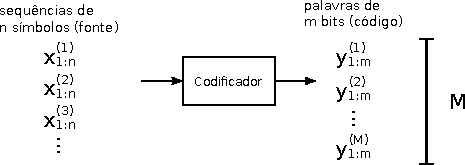
\includegraphics[width=\linewidth]{figures/Mncodes2.pdf}
  \caption{Codificador $(M,n)$, onde $M$ representa o número de mensagens e $n$ o comprimento das sequências.}
  \label{fig:Mncodes2}
\end{marginfigure}

\begin{definition}[Código de Bloco com Taxa Fixa $R$]
Seja $X_1, X_2, \ldots, X_n \sim Q$, i.i.d. mas $Q$ desconhecido. A função do codificador
e decodificador são definidas a seguir:
  \begin{equation}
  \text{codificador: } f_n : \mathcal{X}^n \rightarrow \{1,2,\ldots,2^{nR}\}
  \end{equation}
  \begin{equation}
  \text{decodificador: } \phi_n : \{1,2,\ldots,2^{nR}\} \rightarrow \mathcal{X}^n
  \end{equation}
e a probabilidade de erro
  \begin{equation}
  P_e^{(n)} = Q^n (\{ x_{1:n} : \phi (f_n (x_{1:n})) \neq x_{1:n} \}) .
  \end{equation}
\end{definition}

\begin{definition}[Código de Bloco Universal de Taxa $R$]
  Um código de bloco de taxa $R$ para um fonte é dito universal se a função $f_n$ e $\phi_n$
  não depender da distribuição $Q$ e se
  \begin{equation}
    P_e^{(n)} \rightarrow 0 \text{ quando } n \rightarrow \infty \text{ sempre que } H(Q) < R .
  \end{equation}
\end{definition}

Veremos que, se $R > H(Q)$, então existe uma sequência (em $n$) de códigos com erro evanescente.
Por outro lado, se $R < H(Q)$ a probabilidade de erro vai pra $1$.

Na demonstração do \Cref{thm:teocodshannontipos} utilizaremos ainda a definição de simplex probabilístico.
\begin{definition}[Simplex Probabilístico]
  O Simplex Probabilístico em $\RealNumber^m$ é o conjunto de pontos
  $x_{1:m} = (x_1, x_2, \ldots, x_m) \in \RealNumber^m$ tal que $x_i \geq 0$, $\sum_{i=1}^{m} x_i = 1$.
\end{definition}

\begin{example}[Simplex Probabilístico com $m=2$]
  O Simplex probabilístico será o conjunto de pontos
  \begin{equation}
  \{ (x_1, x_2)  :  x_1 \geq 0 , x_2 \geq 0 , x_1 + x_2 = 1 \} ,
  \end{equation}
  representado na \Cref{fig:prob-simplex-2}.
    \begin{marginfigure}
    \centering
    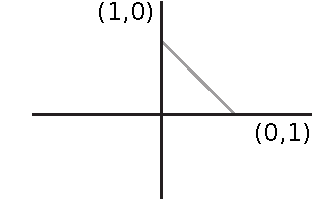
\includegraphics[width=\textwidth]{figures/prob-simplex-2.pdf}
    \caption{Simplex probabilístico para $m=2$.}
    \label{fig:prob-simplex-2}
    \end{marginfigure}
\end{example}

 \begin{example}[Simplex Probabilístico com $m=3$]
  O Simplex probabilístico será o conjunto de pontos
  \begin{equation}
  \{ (x_1, x_2, x_3)  :  x_1 \geq 0 , x_2 \geq 0 , x_3 \geq 0 , x_1 + x_2 + x_3 = 1 \}
  \end{equation}
  representado na \Cref{fig:prob-simplex-3} e com alguns pontos em destaque na \Cref{fig:prob-simplex-3t}.
    \begin{marginfigure}
    \centering
    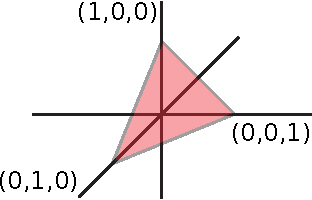
\includegraphics[width=\textwidth]{figures/prob-simplex-3.pdf}
    \caption{Simplex probabilístico para $m=3$.}
    \label{fig:prob-simplex-3}
    \end{marginfigure}

    \begin{marginfigure}
    \centering
    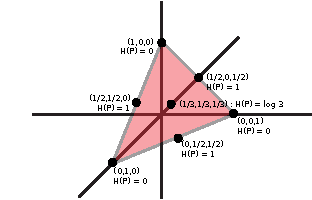
\includegraphics[width=\textwidth]{figures/prob-simplex-types3.pdf}
    \caption{Representação de alguns pontos e suas respectivas entropias.}
    \label{fig:prob-simplex-3t}
    \end{marginfigure}
  \end{example}



O Teorema da Codificação de Shannon é um dos resultados fundamentais da teoria
da informação, estabelecendo as condições sob as quais é possível representar
as informações produzidas por uma fonte i.i.d. com distribuição subjacente $Q$
sem que haja perdas, utilizando, para tanto uma taxa $R$.
O Teorema mostra que, se $R > H(Q)$, então existe um código de bloco universal
para representar a informação produzida pela fonte com probabilidade de erro
tendendo a zero à medida que o comprimento $n$ das sequências aumenta.
Por outro lado, se $R < H(Q)$, não é possível representar a informação da fonte
com probabilidade de erro evanescente.
No contexto do método de tipos, podemos formalizar esse teorema explorando a
estrutura das classes de tipo: como o número de tipos é polinomial em $n$,
enquanto o número de sequências é exponencial em $n$, e apenas os tipos próximos
de $Q$ ocorrem, para $n$ grande, é possível construir códigos universais que
codifiquem eficientemente as sequências produzidas pela fonte, usando aproximadamente 
$nH(Q)$ bits.

\begin{theorem}[Teorema da Codificação de Shannon]\label{thm:teocodshannontipos}
$\exists$ uma sequencia $(2^{nR},n)$ de códigos universais tais que $P_e^{(n)} \rightarrow 0$ para toda
distribuição $Q$ tal que $H(Q) < R$.
\end{theorem}
\begin{proof}
  Fixe $R > H(Q)$. Defina uma taxa para $n$ que é fixada a um fator polinomial:
  \begin{equation}
    R_n \triangleq R - \vert \mathcal{X} \vert \frac{\log (n+1)}{n} < R .
  \end{equation}
  Defina um conjunto de sequências que possuem entropia de tipo menor do que esta taxa:
  \begin{subequations}
    \begin{align}
       A_n &\triangleq \{ x_{1:n} \in \mathcal{X}^n : H(P_{x_{1:n}}) \leq R_n \} \\
           &= \left\{  \bigcup_{P \in \mathcal{P}_n} T(P) : H(P) \leq R_n \right\}
    \end{align}
  \end{subequations}
  A partir desta definição, teremos que
  \begin{subequations}
  \begin{align}
    \vert A_n \vert &= \sum_{P \in \mathcal{P}_n : H(P) \leq R_n} \vert T(P) \vert \leq \sum_{P \in \mathcal{P}_n : H(P) \leq R_n} 2^{nH(P)} \\
                    &\leq \sum_{P \in \mathcal{P}_n : H(P) \leq R_n} 2^{nR_n} \leq (n+1)^{\vert \mathcal{X} \vert} 2^{nR_n} \\
                    &= 2^{n \left( R_n + \vert \mathcal{X} \vert \frac{\log (n+1)}{n} \right)} = 2^{nR} .
  \end{align}
  \end{subequations}
  Como $\vert A_n \vert \leq 2^{nR}$, podemos indexar $A_n$ com $nR$ bits.

  O codificador será dado por
  \begin{equation}
  f_n (x_{1:n}) =
  \begin{cases}
  \text{índice de } x_{1:n} \text{ em } A_n ,     \quad \text{ se } x_{1:n} \in A_n \\
  0                                       ,       \quad \text{ caso contrário }.
  \end{cases}
  \end{equation}
  O codificador associará um índice a $x_{1:n}$ se $H(P_{x_{1:n}}) \leq  R_n$ (ou seja, $x_{1:n} \in A_n$);
  e não associará valor se $H(P_{x_{1:n}}) >  R_n$ (ou seja, $x_{1:n} \notin A_n$).
  Note que $f_n(\cdot)$ não depende da distribuição da fonte, apenas do ordenamento e de $\RealNumber^m$.
  Um erro ocorrerá se $x_{1:n} \notin A_n$.
  Os tipos podem ser representados por pontos em um Simplex Probabilístico, conforme ilustrado na \Cref{fig:type-simplex}.
\begin{marginfigure}%
  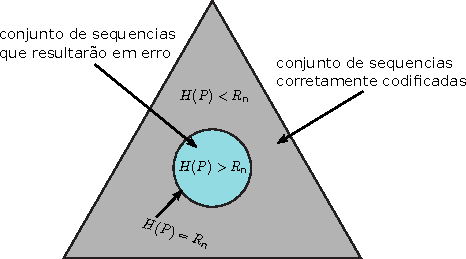
\includegraphics[width=\linewidth]{figures/type-simplex.pdf}
  \caption{Representação das sequências em um simplex probabilísticos. As sequências com $H(P_{x_{1:n}}) \leq  R_n$ não acarretarão em erro no processo de codificação.}
  \label{fig:type-simplex}
\end{marginfigure}
Um erro ocorre quando a sequência não está em $A_n$. Desta forma,
\begin{subequations}
  \begin{align}
  P_e^{(n)} = 1 - Q^n(A_n) &=& Q^n(A^c_n) = \sum_{P: H(P) > R_n} Q^n (T(P)) \\
        &\leq& \sum_{P: H(P) > R_n} \max_{P: H(P) > R_n} Q^n (T(P)) \\
        &\leq& (n+1)^{\vert \mathcal{X} \vert} \max_{P: H(P) > R_n} Q^n (T(P)) \\
        &\leq& (n+1)^{\vert \mathcal{X} \vert} \max_{P: H(P) > R_n} 2^{-n  D(P \mid\mid Q)} \\
        &=& (n+1)^{\vert \mathcal{X} \vert} 2^{-n [\min_{P: H(P) > R_n} D(P \mid\mid Q)]} \label{eq:dempeteoshan}
  \end{align}
\end{subequations}
onde utilizamos que $Q^n(T(P)) \leq 2^{-n D(P\mid \mid Q)}$.
Temos que $R_n$ forma uma sequência crescente com $n$, tal que $R_n < R$ para todo $n$ (veja a \Cref{fig:Rn-seq}).
Por hipótese, $H(Q) < R$. Eventualmente, para algum $n_0$, teremos que $\forall n > n_0$, $R_n > H(Q)$.
Na \Cref{eq:dempeteoshan}, escolhemos $P: H(P) > R_n$.
\begin{marginfigure}%
  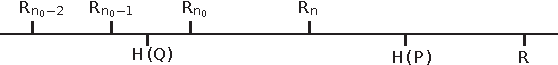
\includegraphics[width=\linewidth]{figures/Rn-seq.pdf}
  \caption{Sequência de taxas $R_n$.}
  \label{fig:Rn-seq}
\end{marginfigure}
Teremos então: $H(P) > R_n > H(Q)$, o que implica em $P \neq Q$.
Desta forma, teremos $D(P \mid\mid Q) > 0$, para $P$ que foi escolhido em \ref{eq:dempeteoshan}.
Teremos assim
\begin{equation}
  P_e^{(n)} \leq \underbrace{(n+1)^{\vert \mathcal{X} \vert}}_{\text{polinomial em } n} \underbrace{ 2^{-n [\min_{P: H(P) > R_n} D(P \mid\mid Q)]} }_{\text{exp. decrescente qnd } n \rightarrow \infty}
\end{equation}
Logo, $P_e^{(n)} \rightarrow 0$ quando $n \rightarrow \infty$.
\end{proof}
Por outro lado, se $R < H(Q)$ teremos $P_e^{(n)} \rightarrow 1$.
A entropia é então o limite de representação, ou compressão.




\chapter{Processos Estocásticos}

Até o momento, nossa análise considerou variáveis aleatórias independentes, uma
simplificação que facilitou a compreensão de conceitos fundamentais como
entropia e informação mútua. Ao final, chegamos à conclusão de que $nH(X)$ bits são
suficientes, na média, para representar uma sequência de $n$ variáveis aleatórias
independentes e identicamente distribuídas. Neste capítulo, removemos essa restrição para
abordar processos estocásticos, nos quais as variáveis aleatórias exibem
dependências temporais ou estruturais. Introduziremos a entropia de um processo
estocástico, que quantifica a incerteza associada a uma sequência de eventos, e
a taxa de entropia, uma medida assintótica da informação gerada por unidade de
tempo. Esses conceitos são essenciais para modelar sistemas dinâmicos. Em
particular, focaremos nas cadeias de Markov, um caso especial de processos
estocásticos em que a dependência é limitada ao estado imediatamente anterior,
oferecendo um equilíbrio entre simplicidade e aplicabilidade em problemas de
codificação e comunicação.

Um processo estocástico estacionário em sentido estrito é uma sequência de
variáveis aleatórias cujas propriedades estatísticas conjuntas permanecem
invariantes sob deslocamentos temporais. Isto implica que, por exemplo, médias,
variâncias e outras estatísticas não dependem do instante absoluto, permanecem
estáveis ao longo do tempo.

\begin{definition}[Processo Estocástico Estacionário (sentido-estrito)]
  Uma sequência de v.a.s. $X_1, X_2, \ldots, X_n$ é governada por uma distribuição probabilística é dita
  estacionária em sentido estrito se
  \begin{equation}
  p(X_{1:n} = x_{1:n}) = p(X_{1+l:n+l} = x_{1:n}) ,
  \end{equation}
  para todo $l$, todo $n$ e todo $x_{1:n} \in \mathcal{X}^n$.
\end{definition}

Um processo de Markov é um processo estocástico em que a probabilidade do
próximo estado depende apenas do estado atual, e não de toda a história
anterior.

\begin{definition}[Processo de Markov de primeira ordem]
  Um processo estocástico é um processo de Markov de primeira ordem se
  \begin{equation}
     p(X_{n+1} = x_{n+1} \mid X_{1:n} = x_{1:n}) = p(X_{n+1} = x_{n+1} \mid X_n = x_n)
  \end{equation}
\end{definition}
A essência de um processo de Markov reside na ideia de que, dado o estado
presente, o futuro e o passado são independentes. Em termos probabilísticos,
para o caso de primeira ordem, isto significa que $p(x_{1:n}) = p(x_1)p(x_2 \mid x_1) \ldots p(x_n \mid x_{n-1})$.
Essa independência condicional reflete a `falta de memória' do processo,
onde conhecer o estado atual basta, não sendo necessário avaliar a influência do passado.

De forma geral, podemos estender a ideia anterior para processos de Markov
de ordens superiores.
\begin{definition}[Processo de Markov de ordem $m$]
  Um processo estocástico é um processo de Markov de ordem $m$ se
  \begin{equation}
    p(X_{n+1} = x_{n+1} \mid X_{1:n} = x_{1:n}) = p(X_{n+1} = x_{n+1} \mid X_n = x_n, X_{n-1} = x_{n-1}, \ldots , X_{n-m} = x_{n-m}) .
  \end{equation}
\end{definition}
Neste caso, isto significa que $p(x_{1:n}) = p(x_{m+1} \mid x_{m}, x_{m-1},
\ldots, p(x_1)) \ldots p(x_{n-1} \mid x_{n-2}, x_{n-3}, \ldots, x_{n-m-1})
p(x_n \mid x_{n-1}, x_{n-2}, \ldots, x_{n -m})$.


Uma cadeia de Markov homogênea é um processo de Markov em que as probabilidades
de transição entre estados não variam com o tempo.
\begin{definition}[Cadeia de Markov homogênea]
  Uma cadeia de Markov é invariante no tempo (também chamada de homogênea) se $p(x_{n+1} \mid x_n)$ não
  depender do tempo, i.e., se
  \begin{equation}
    p(X_{n+1} = b \mid X_{n} = a) = p(X_2 = b \mid X_1 = a) \quad \forall a,b,n .
  \end{equation}
\end{definition}
Neste caso, a cadeia de Markov pode ser descrita por uma matriz de transição fixa $P = [p_{ij}]_{ij}$
em que $p_{ij} = p(X_{n+1} = j \mid X_{n} = i)$. Podemos representar esta cadeia de Markov como um grafo
com setas entre estados cuja probabilidade de transição não é nula.
O fato de ser homogênea também facilita o estudo de propriedades assintóticas,
como a taxa de entropia, como veremos adiante.

\begin{example}[Cadeia de Markov homogênea de primeira ordem]
  Vamos considerar neste exemplo uma cadeia de Markov homogênea de primeira ordem
  com 4 estados. Esta cadeia pode ser ser representada pela sua matriz de transição:
  \begin{equation}
  P = \begin{bmatrix}
          0 & p(2 \mid 1) & 0 & p(4 \mid 1) \\
          0 & p(2 \mid 2) & p(3 \mid 2) & 0 \\
          0 & 0 & 0 & p(4 \mid 3) \\
          0 & 0 & 0 & p(4 \mid 4) \\
          \end{bmatrix} ,
 \end{equation}
 ou, alternativamente, pelo grafo ilustrado na \Cref{fig:markov-example}

\begin{marginfigure}%
  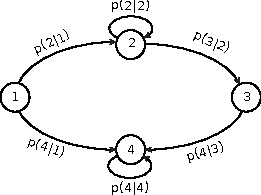
\includegraphics[width=\linewidth]{figures/markov-example.pdf}
  \caption{Exemplo de uma cadeia de Markov de primeira ordem com 4 estados.}
  \label{fig:markov-example}
\end{marginfigure}
\end{example}

Para uma cadeia de Markov homogênea de primeira ordem,
a probabilidade de um estado no instante $n+1$, pode ser dada em função dos possíveis
estados no instante $n$ e da probabilidade de transição:
\begin{equation}
  p(X_{n+1} = i) = \sum_{j} p(X_n = j) p(i|j) ,
\end{equation}
onde $p(i|j)$ é o elemento $p_{ij}$ da matriz de transição $P$. Esta cadeia de
Markov será estacionária se a probabilidade dos estados não mudar
ao longo do tempo, ou seja, $p(X_{n+1} = i) = p(X_n = i)$, para todo $i$.
Quando isto ocorrer, haverá uma distribuição estacionária $\mu$ tal que $\mu P = \mu$, onde $P$ é a matriz de transição.
Isto assegura que a probabilidade de cada estado permaneça constante ao longo do tempo quando o processo parte de,
ou alcança, uma distribuição $\mu$.

\begin{definition}[Cadeira de Markov irredutível]
  Uma cadeia de Markov é irredutível se $p_{ij}(n) > 0$ para todo $i,j$ e para algum $n$ onde
  $p_{ij}(n) = p(X_{n+1} = j \mid X_{n} = i)$.
\end{definition}
Ou seja, qualquer estado é acessível de qualquer outro estado (ao menos em algum instante $n$),
com probabilidade não nula.

\begin{definition}[Período de uma cadeia de Markov]
  Uma cadeia de Markov é periódica se $d(i) > 1$ com
  \begin{equation}
  d(i) = \gcd \{ n : p_{ii}(n) > 0 \}
  \end{equation}
  $d(i)$ é o período do $i$-ésimo estado.
\end{definition}
Note que temos o máximo divisor comum do número de épocas para o qual um retorno ao mesmo estado é possível.


\begin{example}[Cadeia de Markov homogênea de primeira ordem com dois estados]\label{ex:markovsimples2}
  Suponha uma cadeia de Markov homogênea de primeira ordem com apenas dois estados.
  Esta cadeia é caracterizada pela matriz de transição
  \begin{equation}
    P = \begin{pmatrix} 1 - \alpha & \alpha \\ \beta & 1 - \beta \end{pmatrix}
  \end{equation}
  e pode também ser representada pelo grafo da \Cref{fig:markov-example2}.
  \begin{marginfigure}%
  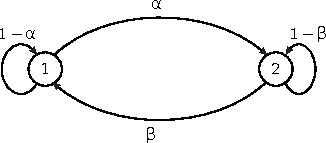
\includegraphics[width=\linewidth]{figures/markov-example2.pdf}
  \caption{Grafo representando uma cadeia de Markov de primeira ordem com dois estados.}
  \label{fig:markov-example2}
  \end{marginfigure}
  Se $\mu = [p_1 \ p_2]^T$ é uma distribuição estacionária, então devemos ter $\mu^T P = \mu^T$.
  Neste caso, teremos
  \begin{subequations}
  \begin{align}
    \mu^T = \begin{pmatrix} p_1 & p_2 \end{pmatrix} &= \begin{pmatrix} p_1 & p_2 \end{pmatrix} \begin{pmatrix} 1 - \alpha & \alpha \\ \beta & 1 - \beta \end{pmatrix} \\
          &= \begin{pmatrix} (1-\alpha) p_1 + \beta p_2 & \alpha p_1 + (1-\beta) p_2 \end{pmatrix}
  \end{align}
  \end{subequations}
  Obtemos assim:
  \begin{equation}
    p_1 = (1-\alpha) p_1 + \beta p_2
  \end{equation}
  logo, $p_1 = \frac{\beta}{\alpha} p_2$.
  Sabemos também que devemos ter $p_1 + p_2 = 1$. Por conseguinte, teremos
  \begin{subequations}
  \begin{align}
    p_1 + p_2 &= 1 \\
    \frac{\beta}{\alpha} p_2 + p_2 &= 1 \\
    p_2 &= \frac{\alpha}{\alpha + \beta} .
  \end{align}
  \end{subequations}
  Assim, teremos
  \begin{equation}
    \mu = \begin{pmatrix} \frac{\beta}{\alpha + \beta} \\ \frac{\alpha}{\alpha + \beta} \end{pmatrix} .
  \end{equation}
\end{example}



A Média de Cesàro representada uma técnica matemática que consiste em
substituir a soma parcial tradicional de uma série por uma média aritmética de
suas somas parciais.
Ela pode ser utilizada para obter representações mais precisas de sinais descontínuos;
reduzir artefatos processamento de sinais; aplicada a equações diferenciais parciais;
e, em processos estocásticos analisar o comportamento assintótico, especialmente ao 
estudar convergência ou taxas de entropia.

\begin{lemma}[Média Cesáro]
  Sejam $a_n$ números reais, se $a_n \rightarrow a$ quando $n \rightarrow \infty$ e $b_n = \frac{1}{n} \sum_{i=1}^n a_i$,
  então $b_n \rightarrow a$ quando $n \rightarrow \infty$.
\end{lemma}

\begin{proof}
  Como $a_n \xrightarrow[ n \rightarrow \infty ]{ } a$, para todo $\epsilon > 0$, existe $N_{\epsilon}$ tal que $\vert a_n - a \vert < \epsilon$
  para todo $n > N_{\epsilon}$.
  Para $n > N_{\epsilon}$ teremos
  \begin{subequations}
  \begin{align}
    \vert b_n - a \vert &= \vert \frac{1}{n} \sum_{i=1}^n a_i - a \vert = \vert \frac{1}{n} \sum_{i=1}^n a_i - \frac{1}{n} \sum_{i=1}^n a \vert \\
                        &= \vert \frac{1}{n} \sum_{i=1}^n (a_i - a) \vert  \leq  \frac{1}{n} \sum_{i=1}^n \vert a_i - a \vert \label{eq:demmediacesaro}\\
                        &= \frac{1}{n} \left( \sum_{i=1}^{N_{\epsilon}} \vert a_i - a \vert + \sum_{i=N_{\epsilon}+1}^n \vert a_i - a \vert \right) \\
                        &\leq \frac{1}{n} \sum_{i=1}^{N_{\epsilon}} \vert a_i - a \vert + \frac{1}{n}  \sum_{i=N_{\epsilon}+1}^n \epsilon \\
                &= \frac{1}{n} \sum_{i=1}^{N_{\epsilon}} \vert a_i - a \vert + \underbrace{\frac{n - N_{\epsilon}}{n}}_{<1} \epsilon \\
                &< \underbrace{ \frac{1}{n} \sum_{i=1}^{N_{\epsilon}} \vert a_i - a \vert }_{< \epsilon } + \epsilon < 2\epsilon \label{eq:demmediacesaro2}
  \end{align}
  \end{subequations}
  onde em \ref{eq:demmediacesaro} utilizamos a desigualdade triangular e em \ref{eq:demmediacesaro2}
  utilizamos o fato de que podemos tomar $n$ grande suficiente de forma que 
  $\frac{1}{n} \sum_{i=1}^{N_{\epsilon}} \vert a_i - a \vert < \epsilon$,
  pois trata-se de uma soma finita.

  Então $b_n \rightarrow a$ quando $n \rightarrow \infty$.
\end{proof}


Processos Estocástico possuem taxas de entropia, que intuitivamente representam o
quantidade de informação nova, na média, que é fornecida pelo processo estocástico a
cada instante.

\begin{definition}[Taxa de Entropia de um processo estocástico]
  A taxa de entropia de um processo estocástico $\{ X_i \}_i$ é definida como
  \begin{equation}\label{eq:txentropia}
    H(\mathcal{X}) \triangleq \lim_{n \rightarrow \infty} \frac{1}{n} H(X_1, X_2, \ldots, X_n) , 
    \end{equation}
quando existir.
\end{definition}

Observe que, na \Cref{eq:txentropia}, quando as v.a.s são i.i.d. teremos $H(X_1, \ldots, X_n) = H(X_1) + \ldots + H(X_n) = n H(X)$ e assim $H(\mathcal{X}) = H(X)$, ou seja,
\begin{equation}
  H(\mathcal{X}) = \lim_{n \rightarrow \infty} \frac{1}{n} H(X_{1:n}) = \lim_{n \rightarrow \infty} \frac{1}{n} \sum_{i=1}^n H(X_i) = H(X_1) .
\end{equation}
A taxa de entropia pode ser vista como a entropia por símbolo para um dado processo estocástico, quando $n$ cresce indefinidamente.



A Taxa de Entropia de um processo estocástico $H(\mathcal{X})$
mede a incerteza média por símbolo em uma sequência longa, 
enquanto a Taxa de Inovação da Informação $H'(\mathcal{X})$,
que será definida a seguir, quantifica a incerteza de um novo símbolo dado o passado. Para
processos gerais, essas taxas podem diferir devido à dependência entre
símbolos; no entanto, em processos estacionários, ambas
convergem ao mesmo valor, ou seja, $H(\mathcal{X}) = H'(\mathcal{X})$,
refletindo a estabilidade estatística do processo ao longo do tempo.

 \begin{definition}[Taxa de Inovação da Informação]
  Vamos assumir um processo estocástico e definir a taxa da seguinte forma
  \begin{equation}
    H'(\mathcal{X}) \triangleq \lim_{n \rightarrow \infty} H(X_n \mid X_{n-1}, X_{n-2}, \ldots , X_1) ,
  \end{equation}
  se existir.
 \end{definition}
 Veremos a seguir que $H'(\mathcal{X})$ existe para um processo estocástico estacionário.

 \begin{theorem}[Um processo estocástico estacionário possui taxa de inovação de informação]
  Para um processo estocástico estacionário, $H(X_n \mid X_{n-1}, X_{n-2}, \ldots , X_1)$ é decrescente com $n$ e possui como limite $H'(\mathcal{X})$.
\end{theorem}
\begin{proof}
  \begin{subequations}
  \begin{align}
  H(X_{n+1} \mid X_1, \ldots, X_n) &\leq H(X_{n+1} \mid X_2, \ldots, X_n) \\
                &= H(X_n | X_1, \ldots, X_{n-1})
  \end{align}
  \end{subequations}
  Onde utilizamos o fato de que condicionar não aumenta (decresce ou não altera) a entropia;
  e utilizamos o fato de que o processo estocástico é estacionário.

  Temos então uma sequência decrescente com limite inferior $0$, logo, esta sequência possui um limite: $H'(\mathcal{X})$.
\end{proof}

\begin{theorem}[Em um processo estocástico estacionário taxa de inovação é igual a taxa de entropia]
  Para um processo estocástico estacionário temos
  \begin{subequations}
  \begin{align}
    \lim_{n \rightarrow \infty} H(X_n \mid X_{n-1}, X_{n-2}, \ldots, X_1) &\triangleq H'(\mathcal{X}) \\
                                                                          &= H(\mathcal{X}) \triangleq \lim_{n \rightarrow \infty} \frac{1}{n} H(X_1,X_2,\ldots,X_n)
  \end{align}
  \end{subequations}
\end{theorem}

\begin{proof}
  \begin{equation}
        b_n = \frac{H(X_1,X_2,\ldots,X_n)}{n} = \frac{1}{n} \sum_{i=1}^n \underbrace{H(X_i \mid X_{i-1}, \ldots, X_1)}_{=a_i} ,
  \end{equation}
  como $a_n \rightarrow H'(\mathcal{X})$, teremos $b_n \rightarrow H'(\mathcal{X})$, mas por definição $b_n \rightarrow H(\mathcal{X})$.
\end{proof}



\begin{example}[Taxa de entropia para cadeia de Markov de primeira ordem]
  A taxa de entropia para um cadeia de Markov de primeira ordem estacionária será dada da seguinte forma
  \begin{subequations}\label{eq:extxentropiamarkov1ord}
  \begin{align}
  H(\mathcal{X}) &= H'(\mathcal{X}) = \lim_{n \rightarrow \infty} H(X_n \mid X_{n-1}, \ldots, X_1) \\
        &= \lim_{n \rightarrow \infty} H(X_n \mid X_{n-1}) \\
        &= H(X_2 \mid X_1) \label{eq:extxentropiamarkov1ordd}\\
        &= - \sum_{x_2, x_1} p(x_2, x_1) \log p(x_2 \mid x_1) \\
        &= \sum_i \mu_i \left[ - \sum_j p_{ij} \log p_{ij} \right] ,
  \end{align}
  \end{subequations}
  onde $\mu$ é a distribuição estacionária, $p_{ij}$ a probabilidade de transição de $i$ para $j$ e,
  em \ref{eq:extxentropiamarkov1ordd}, utilizamos o fato de termos uma cadeia de Marvov de primeira ordem estacionária.
\end{example}

\begin{example}[Markov com apenas dois estados]
  Para a cadeia de Markov simples apresentada no \Cref{ex:markovsimples2}, teremos
  \begin{equation}
    H(\mathcal{X}) = H(X_2 \mid X_1) = \frac{\beta}{\alpha + \beta} H(\alpha) + \frac{\alpha}{\alpha + \beta} H(\beta) .
  \end{equation}
\end{example}


\begin{example}[Modelos de Ehrenfest]
Os Modelos de Ehrenfest são cadeias de Markov que descrevem a dinâmica de
partículas em um sistema com dois compartimentos. Tais modelos são
frequentemente usados para ilustrar conceitos de equilíbrio estatístico e
comportamento assintótico. A análise desse processo estocástico revela
propriedades como estacionaridade e convergência para uma distribuição de
equilíbrio. Paul Ehrenfest propôs um modelo simples para a troca de calor ou
moléculas entre dois corpos isolados. Neste modelo da cadeia de Ehrenfest
iremos considerar a troca de moléculas de gás entre dois compartimentos,
rotulados por 0 e 1, conforme apresentado na \Cref{fig:ehrenfest}.
\begin{marginfigure}%
  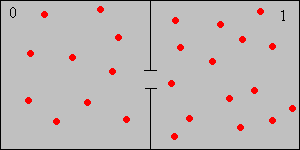
\includegraphics[width=\linewidth]{figures/ehrenfest.png}
  \caption{Exemplo de uma cadeia de Markov de primeira ordem com 4 estados.}
  \label{fig:ehrenfest}
\end{marginfigure}
Partículas movem-se aleatoriamente entre os
compartimentos com probabilidades fixas, e o estado do sistema é representado
pelo número de partículas em um dos compartimentos.
Iremos denotar por $X_k$ o número de partículas no compartimento 1 no instante $k$.
$X_k$ descreve o estado atual do sistema. Temos um processo estocástico gerando $X_{1:n}$,
onde $X_k \in \{0,1,\ldots,m\}$.

Supondo que no instante $k$ o compartimento 1 possua $i$ partículas ($X_k = i$).
O modelo de Ehrenfest nos fornece:
\begin{subequations}
\begin{align}
\Pr(X_{k+1} = i+1 | X_k = i) &= \frac{m - i}{m} , \\
\Pr(X_{k+1} = i-1 | X_k = i) &= \frac{i}{m} .
\end{align}
\end{subequations}

Neste modelo a propriedade de Markov é satisfeita:
\begin{subequations}
\begin{align}
\Pr(X_{n+1} = i+1 | X_0 = i_0, X_1 = i_1, \ldots, X_{n-1} = i_{n-1}, X_n = i) &=& \Pr(X_{n+1} = i+1 | X_n = i) , \\
\Pr(X_{n+1} = i-1 | X_0 = i_0, X_1 = i_1, \ldots, X_{n-1} = i_{n-1}, X_n = i) &=& \Pr(X_{n+1} = i-1 | X_n = i) . 
\end{align}
\end{subequations}
A distribuição condicional não depende de $n$, desta forma, temos um processo estocástico homogêneo.
A cadeia de Markov poderá então ser descrita por uma matriz de transição fixa $P = [p_{ij}]_{ij}$.

Para $m = 4$ teremos a cadeia de Markov representada pelo grafo apresentado na \Cref{fig:ehrenfestm4}.
\begin{figure}%
\begin{tikzpicture}[->, >=stealth', auto, semithick, node distance=2.5cm]
\tikzstyle{every state}=[fill=white,draw=black,thick,text=black,scale=1]
\node[state]    (0)               {$0$};
\node[state]    (1)[right of=0]   {$1$};
\node[state]    (2)[right of=1]   {$2$};
\node[state]    (3)[right of=2]   {$3$};
\node[state]    (4)[right of=3]   {$4$};
\path
(0) edge[bend left,above]   node{$1$}    (1)
(1) edge[bend left,below]   node{$1/4$}  (0)
(1) edge[bend left,above]   node{$3/4$}  (2)
(2) edge[bend left,below]   node{$1/2$}  (1)
(2) edge[bend left,above]   node{$1/2$}  (3)
(3) edge[bend left,below]   node{$3/4$}  (2)
(3) edge[bend left,above]   node{$1/4$}  (4)
(4) edge[bend left,below]   node{$1$}    (3) ;
% edge[loop left]     node{$p^2$}         (1) ;
\end{tikzpicture}
  \caption{Modelo de Ehrenfest com 4 estados.}
  \label{fig:ehrenfestm4}
\end{figure}

Para este modelo, a matriz de transição é
\begin{equation}
\mathbf{P} =
\begin{blockarray}{cccccc}
0 & 1 & 2 & 3 & 4 \\
\begin{block}{(ccccc)c}
  0   & 1   & 0   & 0   & 0   & 0 \\
  1/4 & 0   & 3/4 & 0   & 0   & 1 \\
  0   & 1/2 & 0   & 1/2 & 0   & 2 \\
  0   & 0   & 3/4 & 0   & 1/4 & 3 \\
  0   & 0   & 0   & 1   & 0   & 4 \\
\end{block}
\end{blockarray}
\end{equation}

A distribuição de estado estacionário é tal que $\mathbf{\mu}^T P = \mathbf{\mu}^T$, com $\sum_i \mu_i = 1$.

\begin{subequations}
\begin{align}
\mathbf{\mu}^T P &= \mathbf{\mu}^T \\
\mathbf{\mu}^T (P-I) &= 0 \\
\mathbf{\mu}^T Q &= 0
\end{align}
\end{subequations}


Teremos aqui
\begin{equation}
Q = \begin{pmatrix}
-1  &  1  & 0   & 0   & 0   \\
1/4 & -1  & 3/4 & 0   & 0   \\
0   & 1/2 & -1  & 1/2 & 0   \\
0   & 0   & 3/4 & -1  & 1/4 \\
0   & 0   & 0   & 1   & -1
\end{pmatrix} .
\end{equation}

Vamos incorporar a condição $\sum_i \mu_i = 1$ fazendo:
\begin{equation}
\tilde{Q} = \begin{pmatrix}
-1  &  1  & 0   & 0   & 1 \\
1/4 & -1  & 3/4 & 0   & 1 \\
0   & 1/2 & -1  & 1/2 & 1 \\
0   & 0   & 3/4 & -1  & 1 \\
0   & 0   & 0   & 1   & 1
\end{pmatrix} ,
\end{equation}
e o novo sistema de equações será
\begin{equation}\label{eq-novo-sistema}
\mathbf{\mu}^T \tilde{Q} = (0, 0, 0, 1) .
\end{equation}

Para solucionar a Equação \ref{eq-novo-sistema}, iremos pós multiplicar ambos os lados
pela matriz inversa de $\tilde{Q}$,
\begin{equation}
\mathbf{\mu}^T = (0, 0, 0, 1) \tilde{Q}^{-1} ,
\end{equation}
obtendo assim
\begin{equation}
\mathbf{\mu}^T = \left( \frac{1}{16}, \frac{1}{4}, \frac{6}{16}, \frac{1}{4}, \frac{1}{16} \right)
\end{equation}

Conforme vimos na \Cref{eq:extxentropiamarkov1ord}, a taxa de entropia para um
cadeia de Markov de primeira ordem estacionária será dada da seguinte forma
\begin{equation}
  H(\mathcal{X}) = \sum_i \mu_i H( \mathbf{p_i} ) ,
\end{equation}
onde $\mu$ é a distribuição estacionária,
$p_{ij}$ a probabilidade de transição de $i$ para $j$ (elementos da matriz $P$)
e $\mathbf{p_i}$ a $i$-ésima linha da matriz $P$ (as probabilidades de transição à partir
do estado $i$).

Para o exemplo em questão:
\begin{subequations}
\begin{align}
  H(\mathcal{X}) &= \mu_1 H(\mathbf{p_1}) + \mu_2 H(\mathbf{p_2}) + \mu_3 H(\mathbf{p_3}) + \mu_4 H(\mathbf{p_4}) + \mu_5 H(\mathbf{p_5}) \\
        &= \frac{1}{16} H(0,1,0,0,0) + \frac{1}{4} H(\frac{1}{4}, 0, \frac{3}{4}, 0, 0) + \frac{6}{16} H(0, \frac{1}{2}, 0, \frac{1}{2}, 0) +
                \frac{1}{4} H(0, 0, \frac{3}{4}, 0, \frac{1}{4}) + \frac{1}{16} H(0, 0, 0, 1, 0) \\
        &= 0 + 2 \times \frac{1}{4} \left( \frac{1}{4} \log 4 + \frac{3}{4} \log \frac{4}{3} \right) +
                \frac{6}{16} + 0 \\
        &= \frac{1}{2} \left( \frac{1}{2} + \frac{3}{2} - \frac{3}{4} \log 3  \right) + \frac{6}{16} \\
        &= 1 - \frac{3}{8} \log 3 + \frac{6}{16} = \frac{11}{8} - \frac{3}{8} \log 3 = 0.78064
\end{align}
\end{subequations}

\end{example}


% https://www.overleaf.com/learn/latex/Spacing_in_math_mode
%The different spacing commands in LaTeX math mode serve to fine-tune the spacing between symbols and elements in mathematical expressions. Here’s when you should use each:
%
%### 1. **Thin spaces (`\,` or `\!`)**  
%   - `\,` (thin space, 1/6 of an em): Used to improve readability by slightly separating elements.  
%     - Example: \( a\,b \) (to clarify multiplication without using `\cdot`)  
%   - `\!` (negative thin space, -1/6 of an em): Used to slightly reduce space, often before `d` in differentials.  
%     - Example: \( \int f(x) \,dx \) vs. \( \int f(x)\!dx \)
%
%### 2. **Medium spaces (`\:`, `\;`)**  
%   - `\:` (medium space, 2/9 of an em): Used for slightly larger separation, often in function definitions or cases.  
%     - Example: \( f(x) \:=\: x^2 + 1 \)  
%   - `\;` (thick space, 5/18 of an em): Used to create a noticeable separation, especially in sequences or function application.  
%     - Example: \( f(x) \; g(y) \)  
%
%### 3. **Large spaces (`\quad`, `\qquad`)**  
%   - `\quad` (1 em): Used to separate expressions significantly.  
%     - Example: \( A \quad B \) (for separating terms in an equation)  
%   - `\qquad` (2 em): Used when even more space is needed, often for logical breaks or alignment in displayed math.  
%     - Example:  
%       \[
%       x = a \qquad y = b
%       \]
%
%### **General Guidelines**  
%- Use `\,`, `\!` to fine-tune spacing in integrals, differentials, and multiplication.  
%- Use `\quad` or `\qquad` in displayed equations for logical separation.  
%- Avoid excessive spacing unless necessary for clarity.  


% redundância
% entropia, informação mútua, divergência, capacidade do canal e codificação
%\lipsum[11-20]


%\chapter{Bibliografia}
%\bibliography{tibook}
\printbibliography

\end{document}
